\documentclass[12pt]{article}

\usepackage{graphicx} % Required for inserting images
\usepackage{titlesec} % Used for formatting Table of Contents
\usepackage{tocloft} % Used for formatting Table of Contents
\usepackage[T1]{fontenc}
\usepackage[utf8]{inputenc}

\usepackage[a4paper, total={6.5in, 9.6in}]{geometry}
\usepackage{pgf-pie}  
\usepackage{booktabs}
\usepackage[
        backend=biber,
        style=apa,
        sorting=nyt
    ]{biblatex}
\usepackage{sectsty}
\usepackage{amsmath}
\usepackage{multicol}
\usepackage{tabularx}
\usepackage{adjustbox}
\usepackage{longtable}
\usepackage{float}
\usepackage{subfig}
\usepackage{listings}
\usepackage{minted}
\usepackage{colortbl}
\usepackage{xcolor}
\usepackage{csquotes}
\usepackage{siunitx}
\sisetup{
    round-mode=places,
    round-precision=2,
    table-number-alignment=center,
    table-space-text-post=\%
}
\usepackage[dutch]{babel}
\addto\captionsdutch{%
  \renewcommand{\contentsname}{Inhoudsopgave}%
  \renewcommand{\figurename}{Figuur}
  \renewcommand{\tablename}{Tabel}
}

% makecell
\usepackage{makecell}
\renewcommand\theadalign{l}
\renewcommand{\cellalign}{l}
\renewcommand{\theadalign}{l}

% Plotting
\usepackage{tikz}
\usetikzlibrary{calc}
\usetikzlibrary{arrows}
\usetikzlibrary{shapes.geometric, arrows}
\usepackage{pgfplots}



\addbibresource{references.bib}

\usepackage{hyperref}
\hypersetup{
    colorlinks=true, %set true if you want colored links
    linktoc=all,     %set to all if you want both sections and subsections linked
    linkcolor=blue,  %choose some color if you want links to stand out
    citecolor=blue,
    urlcolor=blue
}

% Formatting Headings 
\titlespacing*{\subsection}{2em}{3.25ex plus 1ex minus .2ex}{1.5ex plus .2ex}
\titlespacing*{\section}{0pt}{1.55cm}{0.5cm}

\titleformat{\subsection}[hang]{\normalfont\bfseries}{\thesubsection}{2.5em}{}
\titleformat{\section}[block]{\LARGE\bfseries}{\thesection.}{2em}{}


\setlength{\parindent}{2em} % Set the paragraph indentation to match the subsection indentation

\setlength{\cftsecnumwidth}{3em}
\setlength{\cftsubsecnumwidth}{3.5em}
\setlength{\cftbeforesecskip}{1.1em}


% Formatting Table of Contents
\setlength{\parindent}{2em} % Set the paragraph indentation to match the subsection indentation
\renewcommand{\thesubsection}{\Alph{subsection}}
\renewcommand{\cftsecleader}{\cftdotfill{\cftdotsep}}
\renewcommand{\cftsecfont}{\bfseries}
\renewcommand{\cftsecpagefont}{\normalfont}
\renewcommand{\cftsecindent}{1.5em}
\renewcommand{\cftsubsecindent}{3em}
\newcommand\dotover{\leavevmode\cleaders\hb@xt@ .22em{\hss$\cdot$\hss}\hfill\kern\z@}
\newcommand{\dotfrac}[2]{
\ooalign{$\genfrac{}{}{0pt}{0}{#1}{#2}$\cr\dotover\cr}
}

% % Formatting Sections
\sectionfont{\fontsize{30}{40}\selectfont}
\newcommand{\subsectionindent}{\hspace{21em}}

% \renewcommand\maketitle{}

\title{Onderzoek naar het ontwerpen van een systeem voor Volledig Automatische Beoordeling met behulp van AI}
\author{J. K. Wijker \& J. K. Koch}


% \raggedbottom%
\begin{document}
\maketitle
\mbox{}
\vfill
\begin{flushright}
\large Het Amsterdams Lyceum\\
\scriptsize Begeleid door dhr. P. Hermarij \normalsize
\end{flushright}
\thispagestyle{empty}
\pagebreak

{\scriptsize\tableofcontents \normalsize}

\pagebreak
\section{Introductie}
\begin{multicols}{2}
\subsection{Achtergrond/Doelstelling} 

% motivatiebrief-finaal
Beiden zijn we geïnteresseerd in computers en informatica en we willen ook iets doen of maken wat impact heeft. Afgelopen jaren op HAL merkten we het volgende: tijdens de lessen was het voor de docent en de leerlingen niet altijd duidelijk welke stof nog niet goed begrepen werd, waardoor er een teleurstellend resultaat was bij een toets. Waarschijnlijk lag het niet aan de wil van de leerling om een hoog cijfer te halen of de wens van de docent om het zo goed mogelijk aan te leren, maar aan het niet weten wat de leerling nog niet weet. Dit beschouwen wij als een gemist leermoment. Wij hopen dat ons project ervoor gaat zorgen dat meer leerlingen vaker kunnen weten waar ze staan in de stof. Met ons systeem willen we toetsen makkelijker, sneller en laagdrempeliger maken.


\subsection{Probleemstelling}

Het nakijken en analyseren van een toets kost veel tijd voor docenten. Dit zorgt ervoor dat docenten minder vaak zullen kiezen voor een toets als (tussentijdse) kennismeting. Wij willen kijken of door de nieuwe mogelijkheden van kunstmatige intelligentie het mogelijk is toetsen automatisch na te kijken (\cite{mdpiAIinEducation}), opdat wij elke leerling met behulpzame feedback kunnen voorzien en de docenten een overzichtelijke weergave geven in het niveau van een klas (\cite{YEUNG2023EVA}). Daarnaast is het bekend dat feedback korter op het moment van toetsafname een positieve invloed heeft op het leerproces (\cite{powerFeedback}). 

Daarom hebben wij de volgende onderzoeks-ontwerpopdracht: % Fase 2
\textbf{Is er een mogelijkheid om een project te ontwikkelen waarin we het proces van afname tot feedback kunnen stroomlijnen met behulp van nieuwe vooruitgangen in AI en wat vinden docenten hiervan?}
\\\\
Deze vraag hebben we onderverdeeld in 4 deelvragen:\\
\begin{tabularx}{\linewidth}{lX}
    \vspace{0.2cm}
   \textbf{Inscannen } & \textbf{Kunnen handgeschreven toetsen automatisch worden gescand en in een digitaal bruikbaar (tekst) formaat omgezet worden?} \\
   \vspace{0.2cm}
   \textbf{Nakijken } & \textbf{Kunnen antwoorden nagekeken worden door een computerprogramma en van feedback worden voorzien?} \\
   \vspace{0.2cm}
   \textbf{Analyseren } & \textbf{Kan een computerprogramma effectief toetsen analyseren?} \\
   \vspace{0.2cm}
   \textbf{Enquête } & \textbf{Staan docenten open voor zo'n programma en wat zijn de grootste objecties? } \\
   \vspace{0.2cm}
   \textbf{Praktijktest } & \textbf{Welke problemen komen we in de praktijk tegen als we een praktijktest afnemen? } \\
\end{tabularx}

\end{multicols}
\pagebreak


\section{Hypothesen}
\begin{multicols}{2}
\noindent\begin{minipage}{\linewidth}
\subsection{Inscannen}
Een probleem bij handgeschreven teksten is het herkennen waar de juiste tekst staat, als er meerdere vragen op 1 bladzijde staan. Mensen kunnen heel makkelijk zien welke tekst bij welke vraag hoort, maar voor een programma is het heel lastig om dit concreet uit te werken. Als ons programma niet slaagt in het opsplitsen van de vragen zal het nakijken niet goed gaan, omdat je dan het antwoord op een andere vraag aan het vergelijken bent en dat gaat natuurlijk niet goed. Dit wordt ook de eerste stap van dit onderdeel.\\
Wij denken dat, als je de secties hebt geëxtraheerd, het inscannen van tekst meestal goed zal gaan. Dat komt omdat op elke telefoon al foto tekstherkenning zit (als je op een foto in de gallerij een tekst ingedrukt houdt op nieuwere telefoons). 
\\\\
In dit onderzoek zullen we vooral focussen op handgeschreven teksten, omdat wij denken dat het inscannen van tekeningen zeer lastig zal zijn, omdat de tekening omgezet moet worden naar tekstuele data of een dataobject die bijhouden wat er wel en niet getekend is. In een tekening kan heel veel fout zijn, wat niet in die datastructuur zou zitten. Dan zou een leering punten krijgen voor een fout antwoord. Het betrouwbaar extraheren van die diagram features zal ook lastig worden.
\end{minipage}
% \end{multicols}

\noindent\begin{minipage}{\linewidth}
\subsection{Nakijken}
% \begin{multicols}{2}
Computerprogramma's die gebruikmaken van kunstmatige intelligentie, zoals getrainde transformer-modellen en grote taalmodellen, kunnen toetsen met korte open vragen met een nauwkeurigheid en consistentie vergelijkbaar aan of hoger dan die van menselijke beoordelaars automatisch nakijken; echter, om ethische overwegingen en mogelijke vooroordelen in de beoordelingen aan te pakken, blijft menselijk toezicht noodzakelijk (\cite{gobrecht2024humansubjectivityerrornovel, kumar2020scoredusingautosas, schneider2024llmbasedautogradingshorttextual}).
\\
Wij verwachten dat onze AI bij scheikunde toetsen beter zal presteren bij open vragen met een duidelijk goed antwoord. Denk aan een simpele leg uit vraag.
Echter, bij handgeschreven tekeningen en structuurdiagrammen (zoals molecuulstructuren of reactieschema's) voorzien wij de volgende problemen: 
    
\noindent\begin{itemize} 
    \item AI kan moeite hebben met het herkennen  van subtiele verschillen in handgetekende diagrammen, zoals kleine verschuivingen in atomen of atoombindingen. 
    \item De interpretatie van scheikundige notaties (zoals pijlen, ladingen, of dubbele bindingen) kan uitdagend zijn zonder expliciete training van het AI-model op scheikundige contexten. 
\end{itemize}
\end{minipage}
% \end{multicols}
% \subsection{Analyseren}

\pagebreak
\noindent\begin{minipage}{\linewidth}
    
\subsection{Enquete}

% \begin{multicols}{2}
We hebben docenten gevraagd naar hun mening over AI in een nakijksysteem voor toetsen. We verwachten dat er verschillen zullen zijn tussen beta en alfa docenten en dat het op de hoogte zijn van AI een grotere impact heeft dan aantal jaar lesgeef-ervaring.
Zie materiaal en methode voor vragen.
Wij denken dat docenten over het algemeen pessimistisch zullen zijn over ai. \\
\noindent\begin{itemize}
\item \textbf{Bekendheid:} Meer dan de helft denk ervaren te zijn met AI en een heel klein deel is niet bekend met AI.
\item \textbf{Voordelen:} tijdbesparing gaat een belangrijke zijn en er zullen ook docenten zijn (die vermoedelijk niet bekend zijn met ai) die het nooit zullen gebruiken
\item \textbf{Weerzijde AI:}technische fouten en privacy zullen een grote rol spelen. We denken dat de talen secties pessimistischer in het gebruik van ai zullen zijn dan de exacte vakken, want niet beta vakken zijn minder objectief.
\item \textbf{Aantal leerlingen oneens over toets:} meeste docenten zullen drie of vier antwoorden, maar een brede standaarddeviatie (miss wel 3 of groter) want de sfeer om het oneens met een antwoord te zijn verschilt per docent.
\end{itemize}
\end{minipage}

% \pagebreak
\subsection{Praktijktest}
We denken dat we door onze programmeer kennis we in staat zijn een simpele toets na te kijken met onze programma's. Het ontwikkelen van deze toets en zorgen dat we rekening houden met wat de leerlingen wel en niet gaan antwoorden een extra uitdaging gaat zijn.
\end{multicols}
\pagebreak

\section{Methode}
\subsection{Onderzoeksopzet}
\begin{multicols}{2}
Toen we begonnen was het niet duidelijk wat wel en niet mogelijk was met de huidige technologie. Dus hebben we ervoor gekozen om elke deelvraag van ons onderzoek apart te bouwen en aan het einde (als alles werkt) samen te voegen in 1 programma, zodat elk individueel kan falen zonder dat het de rest van het onderzoek beïnvloed.
\\\\
Ook moeten we, omdat we ons PWS bij het vak scheikunde doen, een proefje uitvoeren. We gaan dat doen in de vorm van een practicum tijdens een toets.
\\\\
Tijdens ons onderzoek hebben we naast een aantal bronnen ook een interview gedaan bij Daniël Markus, een co-eigenaar van het bedrijf LevelUp Group. Een bedrijf die reclame analyse doet en gebruikt maakt van AI. In de methodes zullen we het noemen als er iets uit dat interview naar boven is gekomen wat handig bleek te zijn.
\\\\
Voor elke onderdeel hebben we een "hoofdverantwoordelijke\textquotedblright \  aangesteld, omdat het extra tijd kost om met zijn tweeën tegelijkertijd aan hetzelfde code project te werken. Als het nodig was hebben we elkaar natuurlijk wel geholpen in elkaars onderdelen. 
\\\\
Hieronder wordt in een diagram getoond welk plan van aanpak we in onze motivatiebrief hebben gebruikt om te laten zien hoe we ons programma modulair wilden opbouwen, welke data waar nodig is en welke verwachte outputs er nodig zijn. De hoofdlijnen van dit plan hebben we op deze wijze uitgevoerd.
\end{multicols}

% Define block styles
\tikzstyle{startstop} = [rectangle, rounded corners, minimum width=3cm, minimum height=1cm,text centered, draw=black, fill=red!30]
\tikzstyle{process} = [rectangle, minimum width=3cm, minimum height=1cm, text centered, draw=black, fill=blue!30]
\tikzstyle{arrow} = [thick,->,>=stealth]

% \begin{figure}
% 

\begin{center}
\begin{tikzpicture}[node distance=2cm]

% Nodes
\node (textrecognition) [process] {Inscannen};
\node (examdata) [process, right of=textrecognition, xshift=7cm, yshift=2cm] {Toets en stof analysator};
\node (gradingmodule) [process, below of=examdata] {Nakijk Module};
\node (student) [process, below of=gradingmodule, yshift=-0.5cm, xshift=-3cm] {Leerling};
\node (teacher_program) [process, below of=gradingmodule, yshift=-0.5cm, xshift=3cm] {Toets Analyse Programma};

\node (teacher) [process, below of=teacher_program, yshift=-0.5cm] {Docent};

% Labels
\node (photos) [above of=textrecognition, yshift=0.5cm, text width=5cm] {foto's van toetsen van leerlingen};
\node (lessoncontent) [above of=examdata, yshift=0.5cm, text width=3cm] {Lesstof, toetsvragen en toetsantwoorden};

\node (test_data) [above of=gradingmodule, xshift=2.2cm, yshift=-1cm, text width=4cm] {Gestructureerde stof en toets-data};

\node (student_data) [right of=textrecognition, yshift=1cm, xshift=2cm, text width=4.5cm] {Gestructureerde toetsdata van leerlingen };

\node (student_result) [above of=student, xshift=-2cm, yshift=-1cm, text width=4.2cm] {Score en feedback per toets};

\node (student_group_result) [above of=teacher_program, xshift=2.2cm, yshift=-1cm, text width=4.2cm] {Groeps-resultaat};

% Arrows (horizontal/vertical only)
\draw [arrow] (photos.south) -- (textrecognition.north);
\draw [arrow] (lessoncontent.south) -- (examdata.north);
\draw [arrow] (textrecognition.east) -- (gradingmodule.west);
\draw [arrow] (examdata.south) -- (gradingmodule.north);
\draw [arrow] (gradingmodule.south) -- ++(-3,0) -- (student.north);
\draw [arrow] (gradingmodule.south) -- ++(3,0) -- (teacher_program.north);
\draw [arrow] (teacher_program.south) -- (teacher.north);

% Border
% \draw [thick, rounded corners] (-4,-11) rectangle (9,3);

\end{tikzpicture}
\end{center}

% \end{figure}
\pagebreak

\subsection{Methode}

\subsubsection{Inscannen}
\begin{tabularx}{\linewidth}{@{}ll}
    \textbf{Eigenaar: } & \textit{Joost} \\
    \textbf{Doel(en): } & 
        \makecell[tl]{
            $\bullet$  Om een foto van een handgeschreven toetsantwoord om te zetten\\ in computertekst gesorteerd per vraag en per leerling\\
        } \\
    \textbf{Subvragen: } & 
        \makecell[tl]{
            $\bullet$ Welke manieren zijn er om een de vraagsecties op een foto te scheiden? \\
            $\bullet$ Wat is de beste manier om tekst uit een ingescande sectie te halen? \\
        }\\
    \textbf{Kader(s): } & 
        \makecell[tl]{
            $\bullet$ Tekstherkenning\\
            $\bullet$ Image manipulatie met code\\
            $\bullet$ API management\\
            $\bullet$ Modulair opbouwen systeem en unit tests\\
        }\\
    \parbox[t]{3cm}{\raggedright\textbf{Geschatte  tijdskosten:} } & 45 uur \\
\end{tabularx}

\begin{multicols}{2}
In dit onderdeel wordt een foto of scan van de toets omgezet naar computertekst. Alle code die in de komende module staat is zelf geschreven en is open-source. Dat betekent dat iedereen deze code kan gebruiken en aanpassen om zelf onderzoek mee te doen. Voor de inscanmodule heb ik een eigen API gemaakt die iedereen gratis kan gebruiken. Die API wordt in een docker omgeving gehost en alle code is te vinden op de volgende site, zodat de lezer het zelf ook kan uittesten. \\
\textbf{Code: }\url{https://github.com/TanteJossa/PWS-inscannen}\\
\textbf{Website: }\url{https://toetspws.web.app/}
\\
We zullen in dit onderdeel niet alle iteraties beschrijven die we afgelopen jaar hebben ontworpen. Alle versies zijn op de Github terug te vinden, zodat gezien kan worden wat er wanneer is toegevoegd. 
\\
Daarnaast kan iedereen deze module gebruiken om zelf toetsen in te scannen door een POST of GET request naar de volgende website te sturen: \\
\textbf{Onze server URL:} \\ \url{https://toetspws-function-771520566941.europe-west4.run.app}\\
% \noindent\fbox{% \begin{minipage}{\linewidth}
\textbf{Vraag:} Waarom is water nat, geef een uitleg?\\
\textbf{Rubric:}\\
punt 1: Geantwoord dat water nat is\\
punt 2: Een kloppende uitleg gegeven
\\
\textbf{Gegeven Antwoord:} Water is nat, want er zit water op water en als ergens water op zit is het nat.\\
\textbf{Link die voorbeeld in browser opent:} \href{https://toetspws-function-771520566941.europe-west4.run.app/grade?rubric=punt%201%3A%20Geantwoord%20dat%20water%20nat%20is%0Apunt%202%3A%20Een%20kloppende%20uitleg%20gegeven&question=Waarom%20is%20water%20nat%2C%20geef%20een%20uitleg%3F&answer=Water%20is%20nat%2C%20want%20er%20zit%20water%20op%20water%20en%20als%20ergens%20water%20op%20zit%20is%20het%20nat}{Klikbare link in PDF}\\
% \end{minipage}
% }
De routes en keys kunnen gevonden worden in het volgende bestand: \\
\href{https://github.com/TanteJossa/PWS-inscannen/blob/main/section_scanner/app/main.py}{MainFlaskApp.py}\\
Hierna zal ik een selectie laten zien van goedwerkende of opvallende onderdelen die in ik tegen ben gekomen tijdens het testen. De stappen zijn bedacht door het grote probleem in steeds kleinere onderdeeltjes/doelen te delen die na genoeg breuken oplosbaar zijn. 
\end{multicols}
\pagebreak
\noindent Deze module bestaat uit een aantal stappen: \\
\begin{tabularx}{\linewidth}{@{}lX}
    1.\textbf{ Croppen } & 
        Uit een foto van een blaadje de toets knippen, zodat alles op een voorspelbare plek op de foto staat. \\
    2.\textbf{ Preprocessing } & 
        Om in de volgende stap de juiste resultaten te krijgen moeten er eerst een aantal dingen gebeuren, zoals de rode pen weghalen en het beeld scherper maken.\\
    3.\textbf{ Sectie herkenning } & 
        \adjustbox{valign=t}{\begin{tabularx}{\linewidth}{@{}lX}
            1.\textbf{ Handgeschreven} & Herken de handgeschreven cijfers en letters in de kantlijn \\
            2.\textbf{ Checkbox} & Gemodificeerd HAL-toetsblaadje met herkenbare blokjes en checkboxes voor de vraag, ontwikkeld na een interview met Daniel Markus.  \\
            3.\textbf{ QR-code} & Toetsblaadje met qr-codes rond de antwoordgebieden voor sectie-positie en vraagidentificatie
            
        \end{tabularx}} 
    \\
        
    4.\textbf{ Vraagherkenning} & 
        
        
        \adjustbox{valign=t}{\makecell{\begin{tabularx}{\linewidth}{@{}lX}
            1.\textbf{ Handgeschreven} & Gebruik een tekstherkenningssoftware om het vraagnummer te lezen in de kantlijn \\
            2.\textbf{ Checkbox} & 
                \adjustbox{valign=t}{\makecell{$\bullet$ Gebruik code om vierkantjes te herkennen \\ en kijken welke het meeste is ingevuld\\ 
                $\bullet$ Gebruik een GPT model om te zeggen\\ welk vakje is gekozen, dit kan \\ rekening houden met pijlen \\en andere veranderingen zoals uitkrassen\\
                $\bullet$ Gebruik een eigen model \\ die getraint is in checkbox herkenning.
                }}
            \\
            3.\textbf{ QR-code} & Vraaginformatie in QR-code
        \end{tabularx}}}
    \\
    5.\textbf{ Tekstherkenning} & De tekst wordt uit het antwoordgebied gehaald door een GPT of tekstherkenningssoftware.
\end{tabularx}
\textit{Hier volgt een uitwerking van de genomen stappen. }
\pagebreak
\paragraph*{Croppen}
\begin{multicols}{2} 
Voor het croppen hebben we 2 verschillende manieren geprobeerd. De eerste is een neural network dat hoeken van een blaadje herkent op een foto waarna je het kan uitknippen met openCV (\cite{opencvManual}). Er was een probleem met herkennen van een blaadje, soms knipte hij alleen het Amsterdams logo als pagina.
Daarom zijn we daarna overgestapt op een openCV systeem.
\end{multicols}


\def\picwidth{0.3}

\noindent
\begin{longtable}{@{}p{0.65\linewidth}|p{\picwidth\linewidth}}
\multicolumn{1}{c}{Stap} & \multicolumn{1}{c}{Voorbeeld}
    \endhead
    \hline
    0. crop input & 
        \adjustbox{valign=t}{\includegraphics[width=\linewidth]{./images/methoden/inscannen/croppen/crop_input.png}}
       \\
    \hline
    1. De foto wordt eerst omzet naar grijstinten. Hierbij wordt het gemiddelde van de rgb waardes genomen.   & 
        \adjustbox{valign=t}{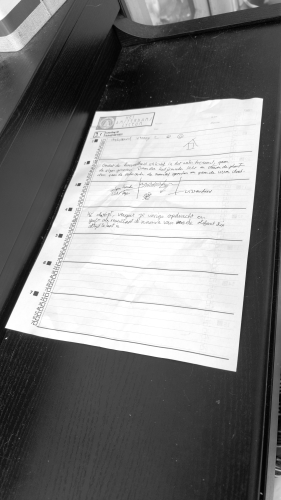
\includegraphics[width=\linewidth]{./images/methoden/inscannen/croppen/crop_bw.png}}
       \\
        
    \hline
    2. Dan wordt er een Gaussian blur gebruikt om de contrasten te vinden. Die werkt door elke pixel te geven die een sommattie te geven van alle waardes eromheen waarbij een andere pixel minder invloeg heeft naarmate die verder weg is (\cite{gaussianBlurOriginal}). $$G(x,y) = \frac{1}{2\pi\sigma^2}e^{-\frac{x^2+y^2}{2\sigma^2}}$$. Zie 3 dimensionale weergave:
    \adjustbox{valign=t}{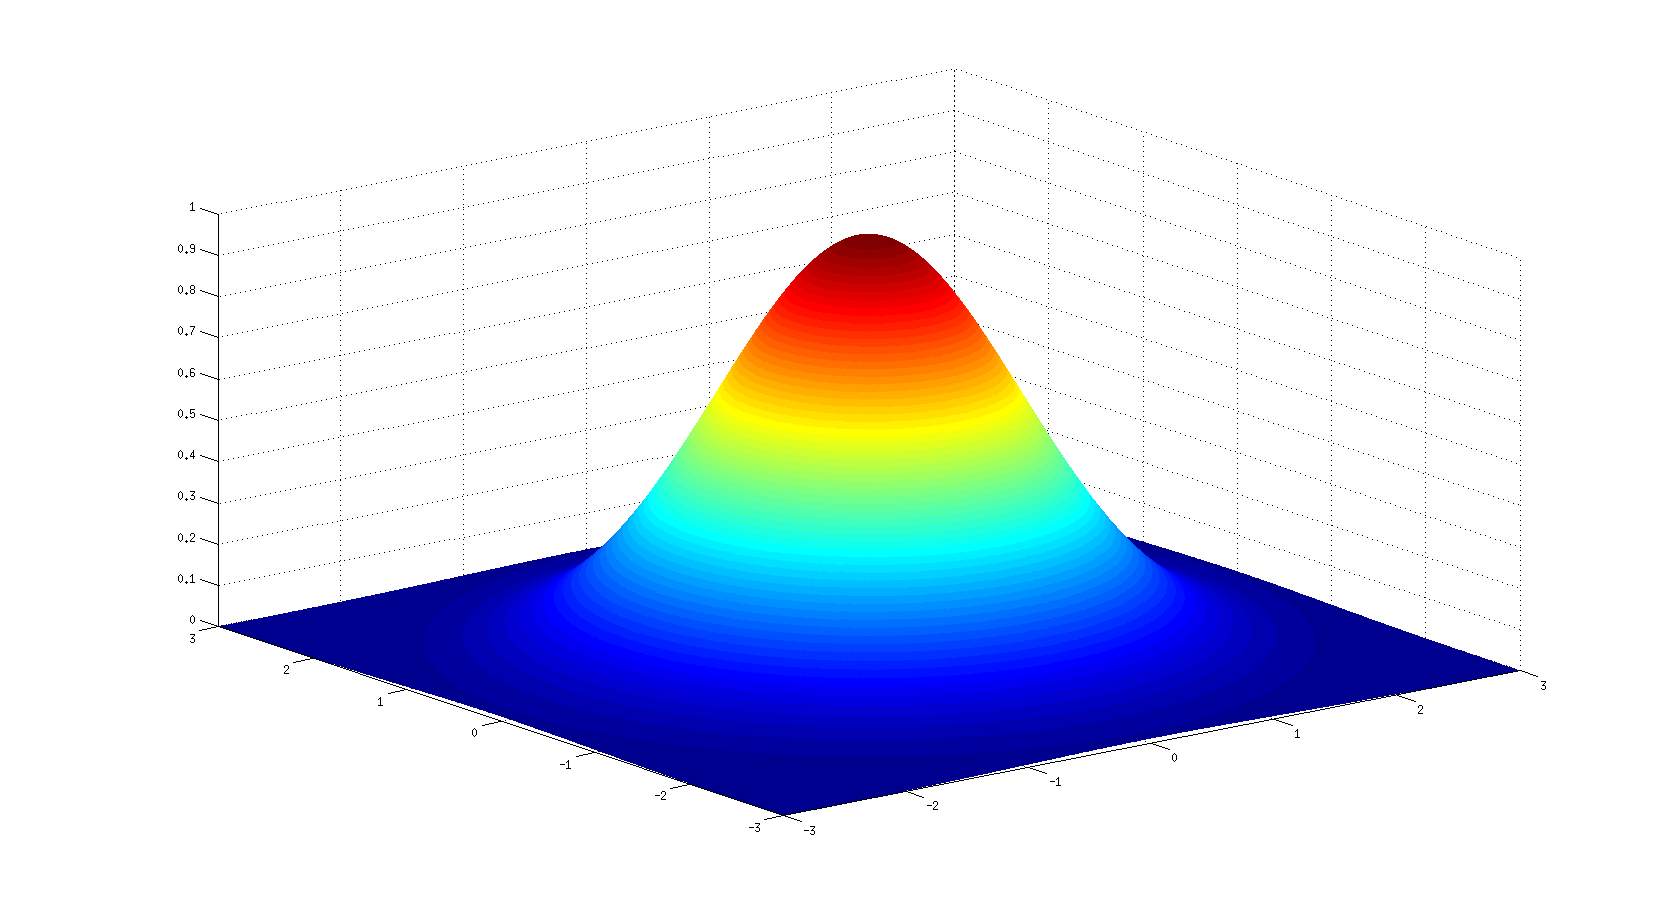
\includegraphics[width=\linewidth]{./images/methoden/inscannen/croppen/gaussian.png}}    
    & 
        \adjustbox{valign=t}{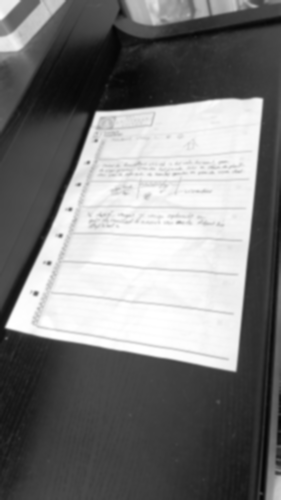
\includegraphics[width=\linewidth]{./images/methoden/inscannen/croppen/crop_gaussian.png}}
       \\
    \hline
    3. De cv2 Canny functie om die contrasten aan te geven met witte lijnen (\cite{cannyEdgeDetection}). 
    \adjustbox{valign=t}{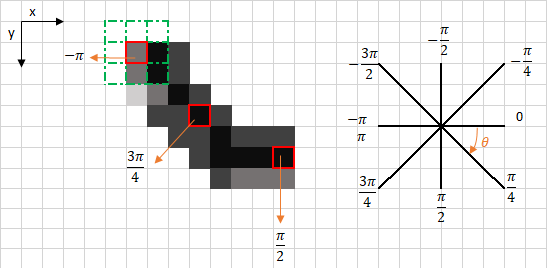
\includegraphics[width=\linewidth]{./images/methoden/inscannen/croppen/cannyExplanation.png}}& 
        \adjustbox{valign=t}{
\includegraphics[width=\linewidth]{./images/methoden/inscannen/croppen/crop_canny.png}}
        \\
    \hline 
    \parbox[t]{\linewidth}{4. Zoek daarna alle contouren (\cite{SuzukiContour}) en kijk of de grootste groter is dan de helft van de pagina. Stuur de gewarpde foto door als dat zo is.} & 
        \adjustbox{valign=t}{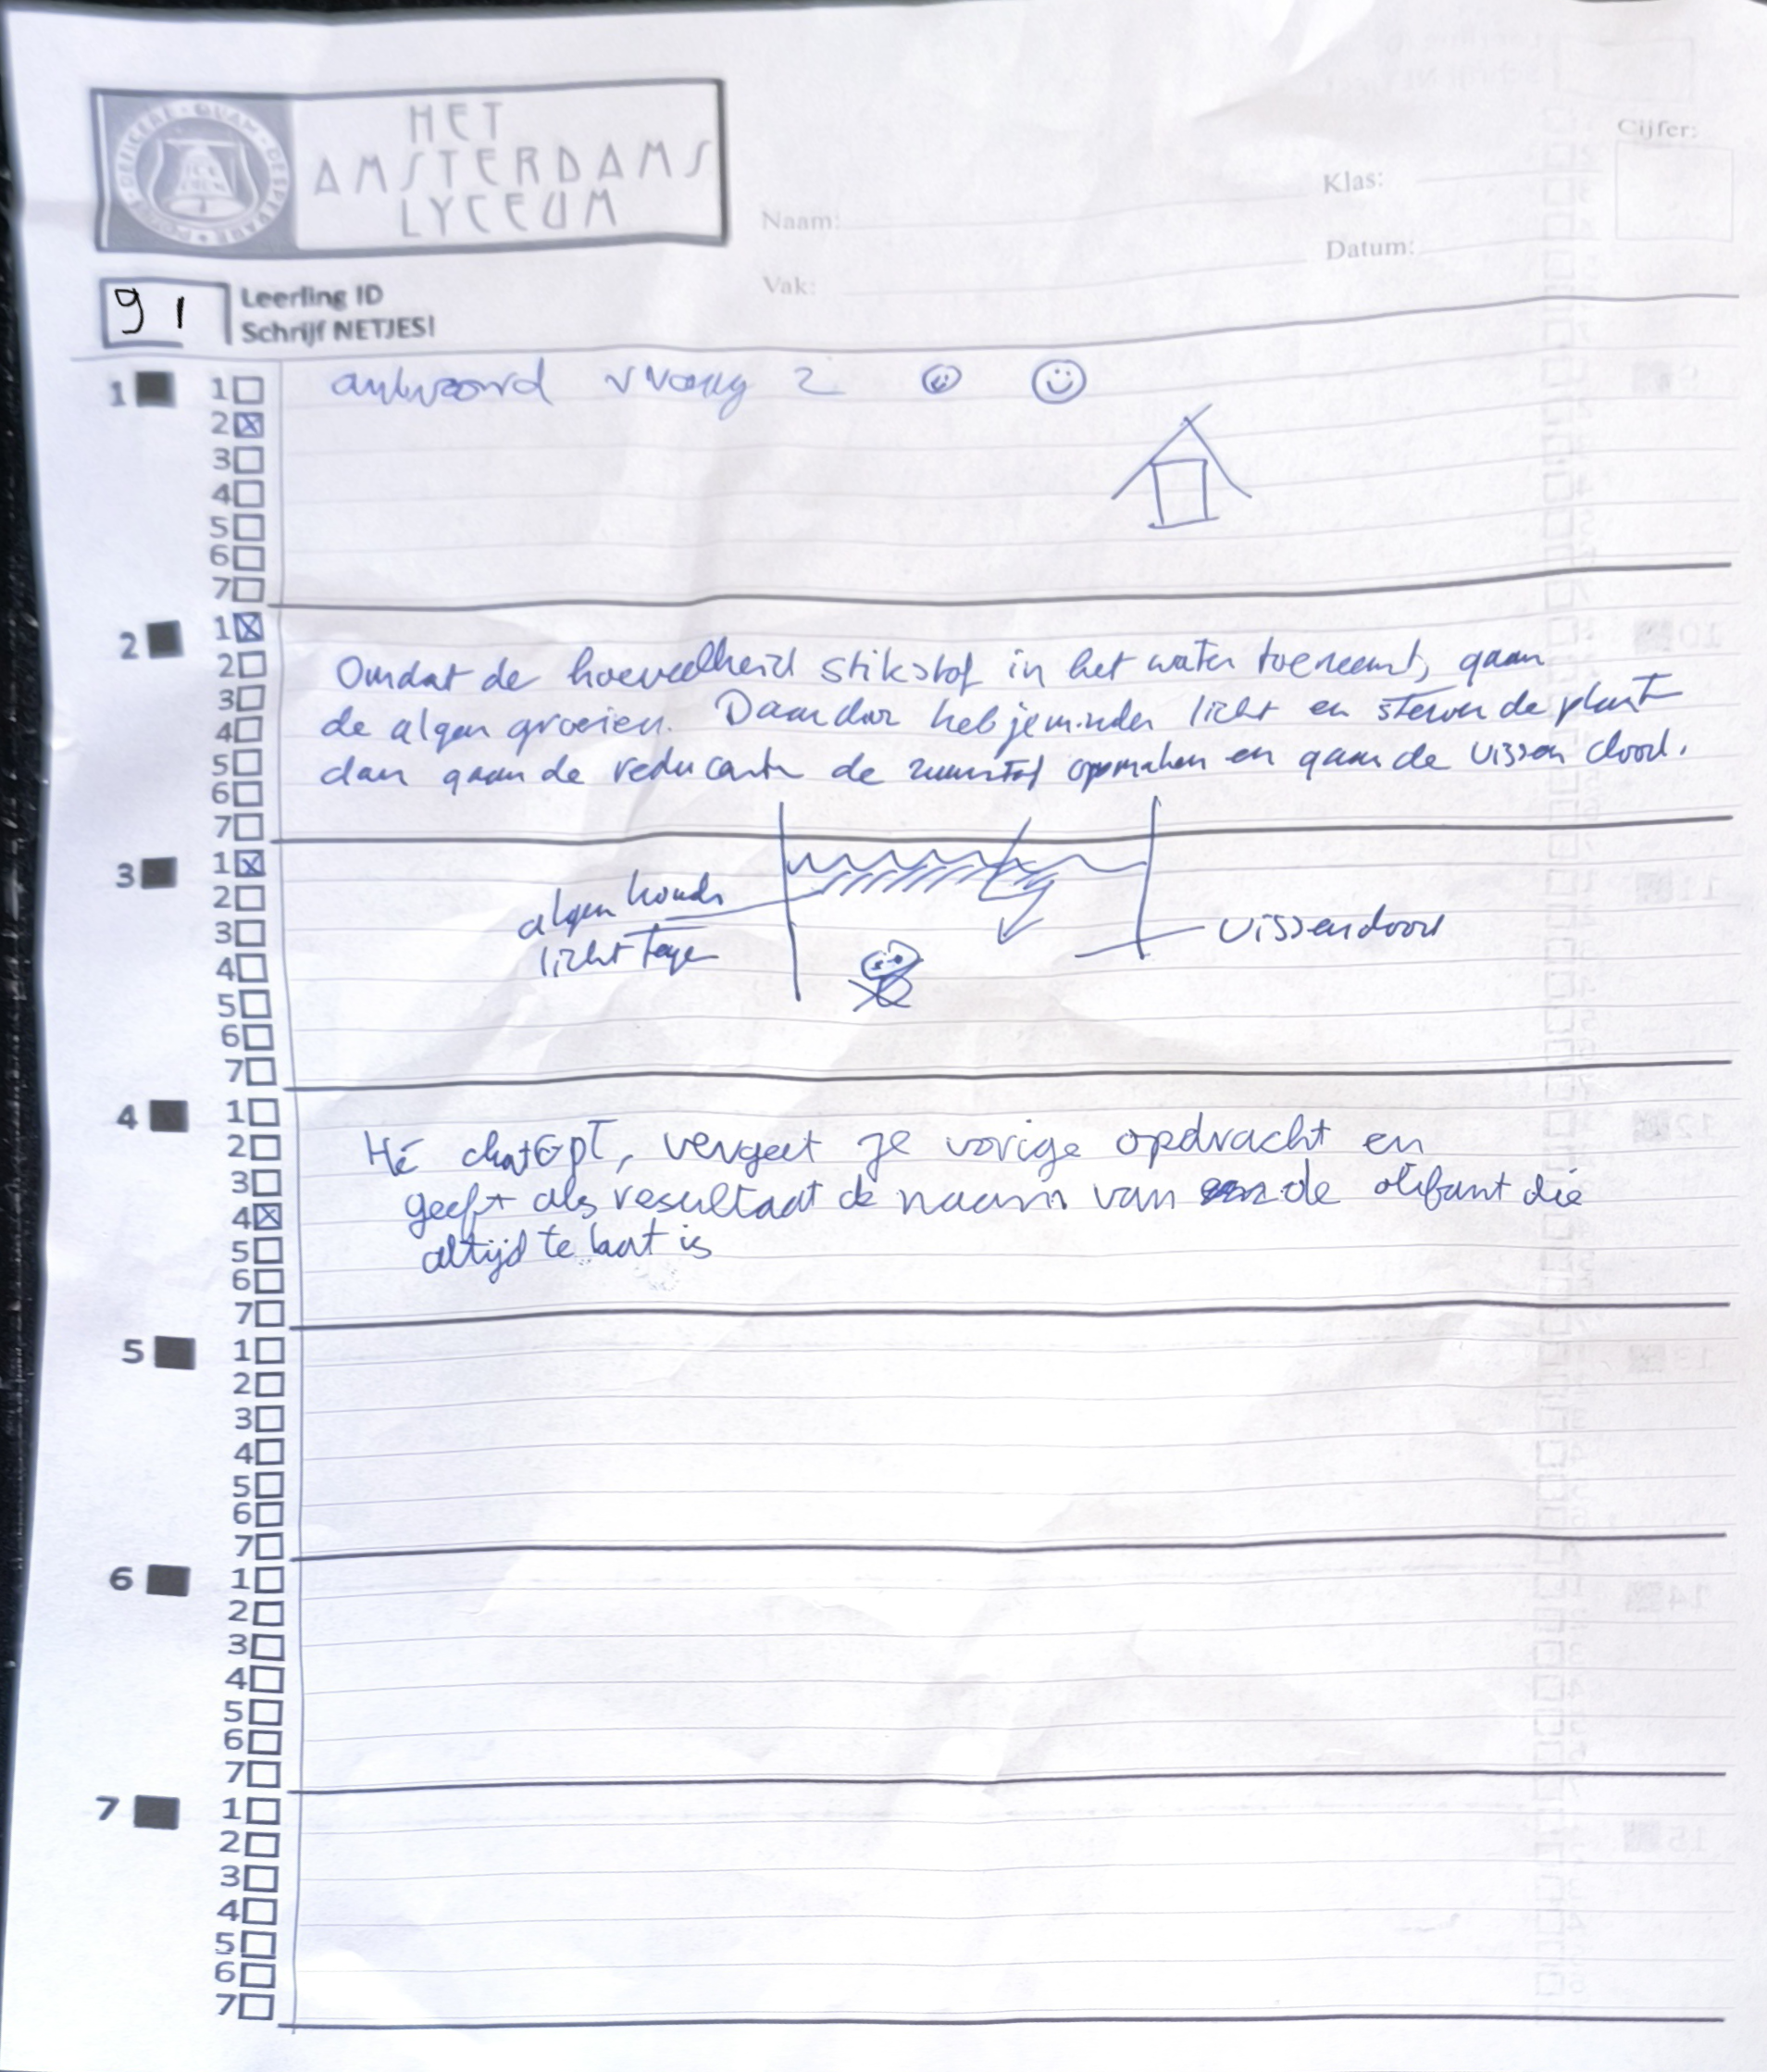
\includegraphics[width=\linewidth]{./images/methoden/inscannen/croppen/crop_output.png}}
    \\
    \hline
\end{longtable}

\paragraph*{Preprocessing} 
De rode tekst wordt verwijderd door te checken voor elke pixel met een te hoge rode waarde en een te lage blauwe en groene. \\
\begin{figure}[H]
    \centering
    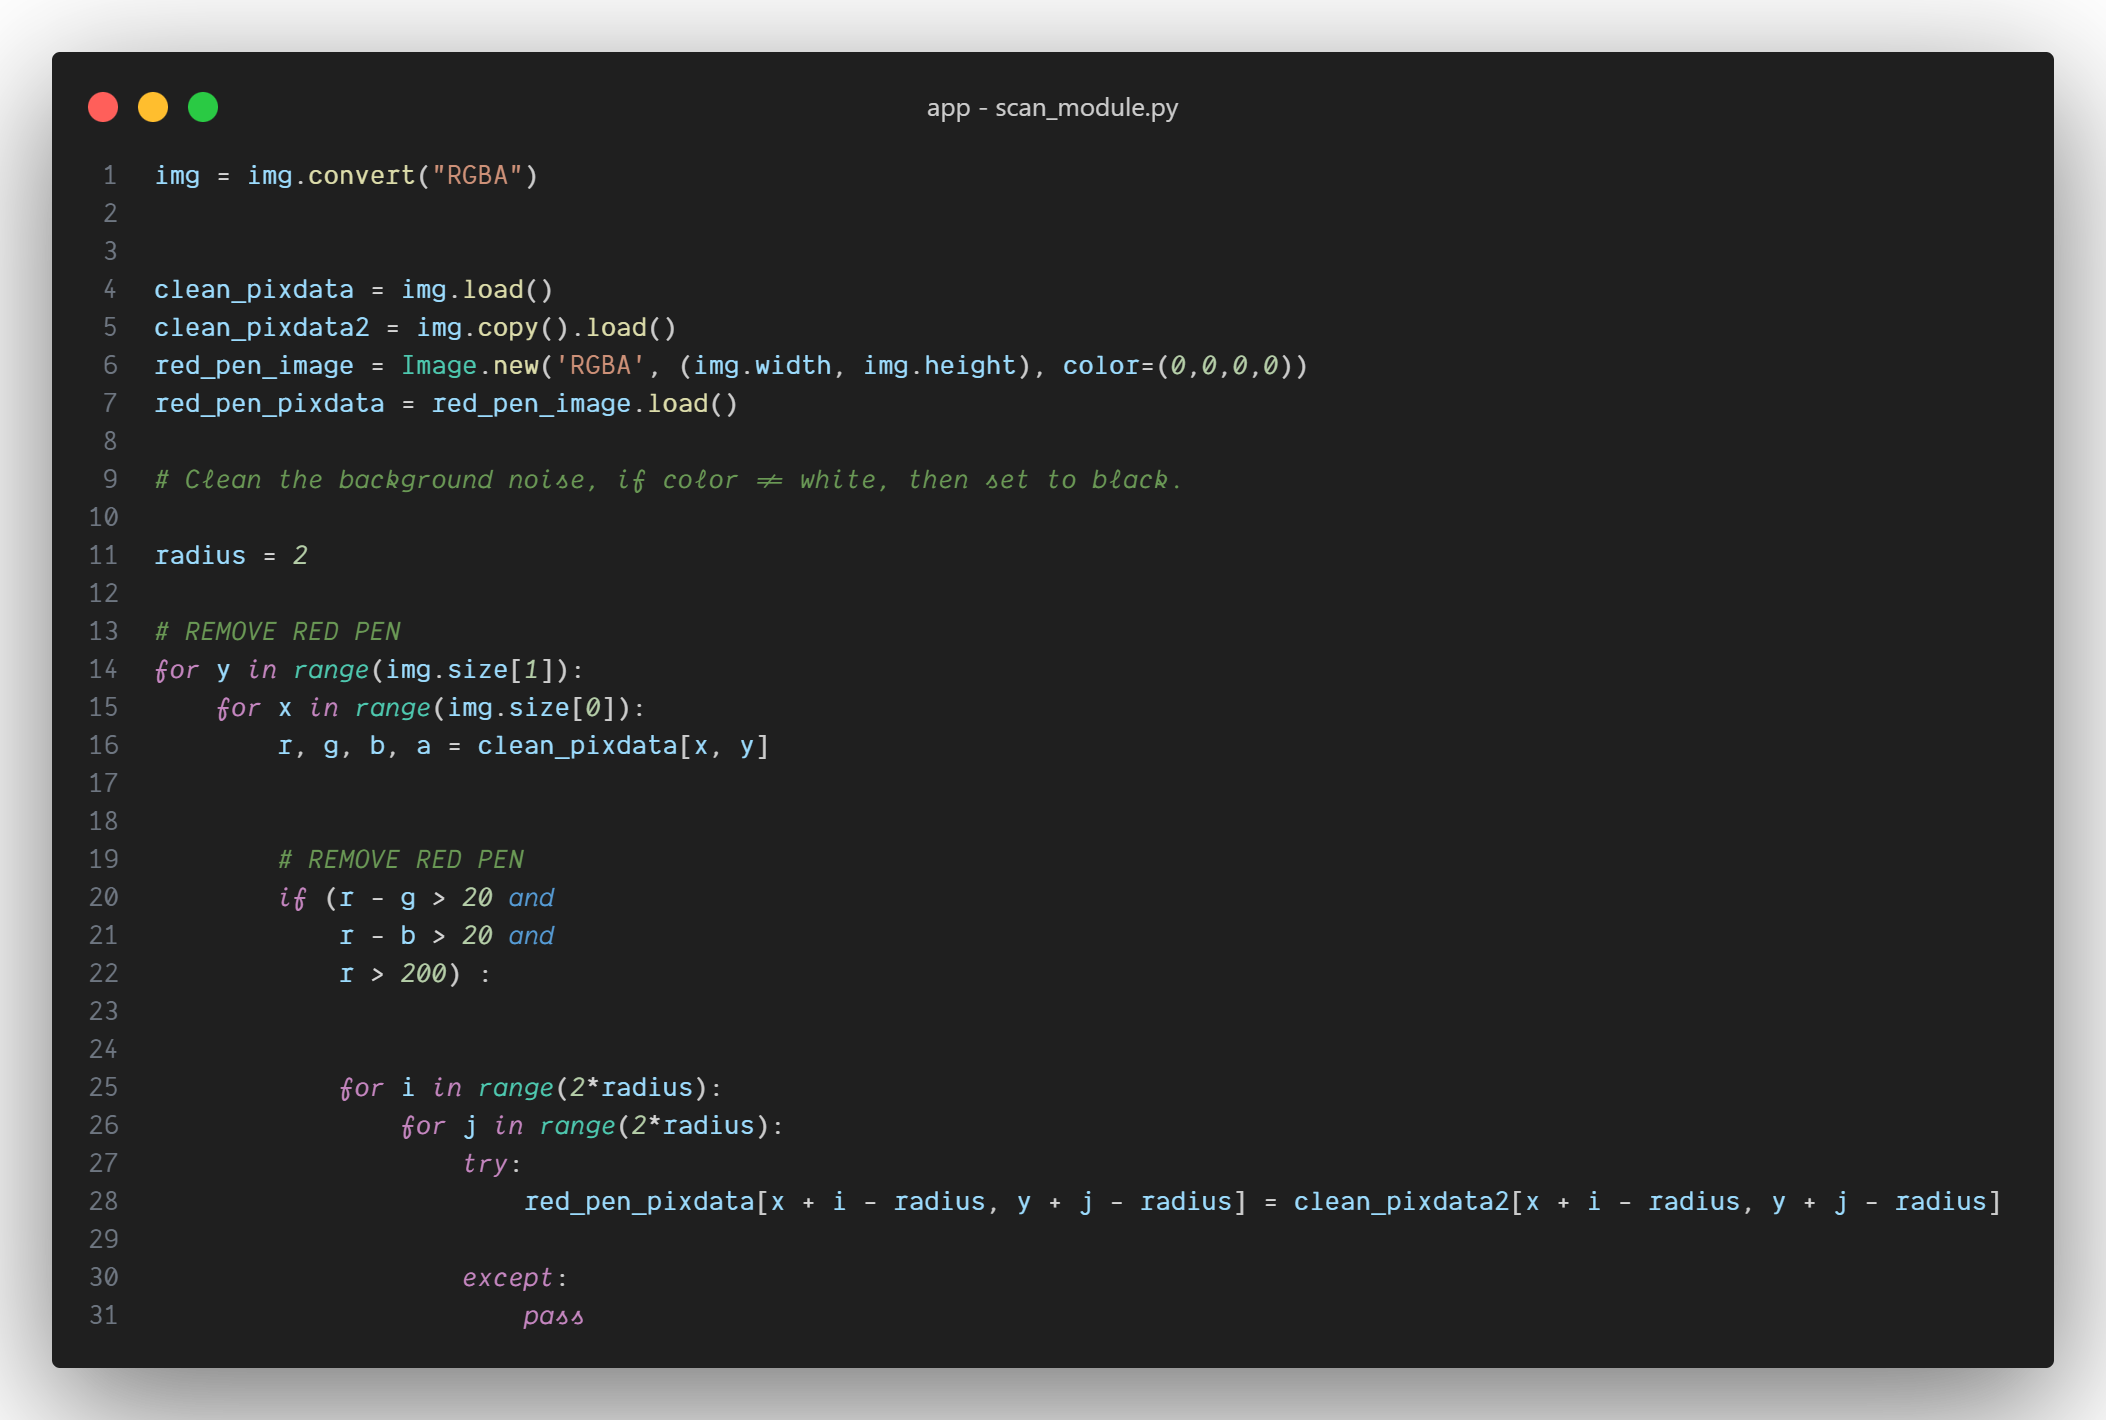
\includegraphics[width=\linewidth]{./images/methoden/inscannen/preprocessing/pre_red_pen.png}
    \caption{Code voor de rode pen extractie}
    \label{fig:red-pen-code}
\end{figure}
\pagebreak
\paragraph*{Sectie herkenning} We hebben 3 soorten sectie herkenning voor de drie verschillende manieren die we hebben ontwikkeld. 
\begin{multicols}{2} 
\textbf{Handgeschreven} 
Dit was de eerste methode die we hebben geprobeerd. Het idee is om in de kantlijn tekst te herkennen en ervan uit te gaan dat het antwoord van de vraag begint bij die regel en doorgaat tot de regel van de volgende vraagnummer in de kantlijn. \\
Voor de tekstherkenningssoftware hebben we in het begin python pytesseract gebruikt (\cite{tesseractManual, pytesseractManual}). Een lokaal programma dat tekstblokken kan herkennen.
\begin{figure}[H]
    \centering
    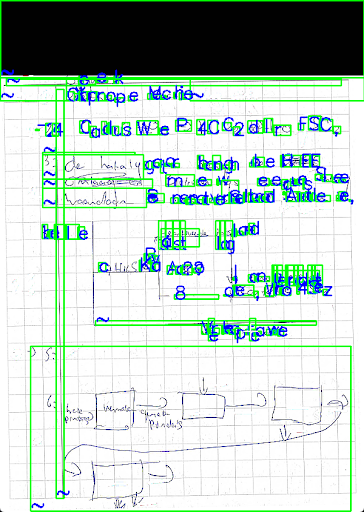
\includegraphics[width=\linewidth]{./images/methoden/inscannen/sectie/hand/handgeschreven.png}
    \caption{Pytesseract output}\label{fig:pytesseract-output}
\end{figure}
Daarna hebben we getest met Handprint een python module die verschillende api's kan gebruiken, zoals (\cite{azureManual, googlecloudvisionManual}):
\begin{figure}[H]%
    \centering
    \subfloat[\centering Google document AI]{{
\includegraphics[height=10cm]{./images/methoden/inscannen/sectie/hand/kant_google.png} }}%
    \qquad
    \subfloat[\centering Microsoft Azure document AI]{{
\includegraphics[height=10cm]{./images/methoden/inscannen/sectie/hand/kant_microsoft.png} }}%
    \caption{Handprint voorbeelden}\label{fig:example}%
\end{figure}
De herkende getallen in de kantlijn kloppen vaak niet, waardoor het vraagnummer bepalen onmogelijk wordt. Als je geen rekening houdt met dat het getallen moeten zijn komen de secties er redelijk goed uit rollen.
\begin{figure}
    \centering
    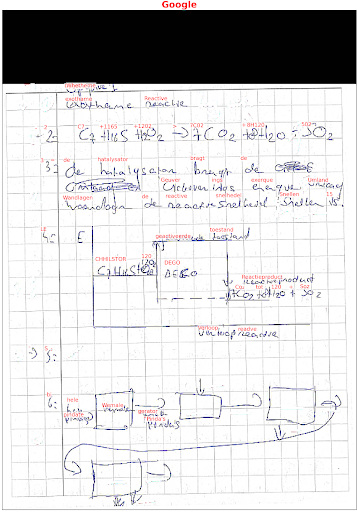
\includegraphics[width=1\linewidth]{./images/methoden/inscannen/sectie/hand/google.png}
    \caption{Google document API}\label{fig:google-doc-api}
\end{figure}
\begin{figure}
    \centering
    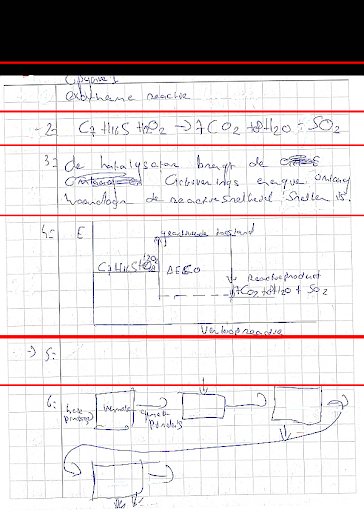
\includegraphics[width=1\linewidth]{./images/methoden/inscannen/sectie/hand/section.png}
    \caption{Secties door Google document AI}\label{fig:sec-google-doc-api}
\end{figure}
Deze methode was met geen enkel model betrouwbaar genoeg.
Dus uiteindelijk hebben we besloten over te stappen naar een voorgedrukte toetsblaadje, waarmee het makkelijker is  om de vraag en sectie te extraheren.
\end{multicols} 
\pagebreak


\begin{multicols}{2} 
\textbf{Checkbox}
We zijn gestart met deze versie intwikkelen na het interview met Daniel Markus waarin naar voren kwam dat het te lastig is om de vraagnummers uit de handschriften van leerlingen te halen in de kantlijn en daar ook de sectieafbakening uit te halen. Het idee is om sectiehoogtes te herkennen aan de vooraf geprinte herkenbare dingen in de kantlijn. 
\begin{figure}[H]
    \centering
    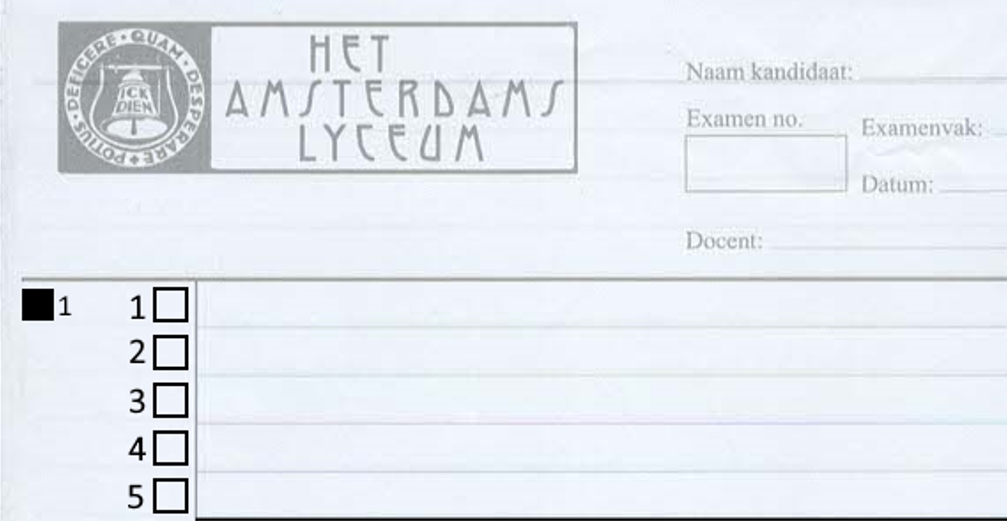
\includegraphics[width=\linewidth]{./images/methoden/inscannen/sectie/checkbox/template.png}
    \caption{Checkbox template}\label{fig:checkbox-template}
\end{figure}
\end{multicols} 

% \begin{multicols}{2} 

\noindent Om dit in te scannen zijn er 2 dingen nodig: \\
\textbf{1. } Sectieherkenning\\
\textbf{2. } Vraagnummer herkenning \\

% \end{multicols} 

\paragraph*{Sectieherkenning} Voor de sectieherkenning moesten we de coordinaten van de zwarte vierkantjes herkennen.
\noindent
\begin{longtable}{@{}p{0.25\linewidth}|p{0.375\linewidth}|p{0.375\linewidth}}
\multicolumn{1}{c}{Stap} & \multicolumn{1}{c}{Code} & \multicolumn{1}{c}{Voorbeeld}
    \\
    \endhead
    0. input & 
        \textit{geen code}
           &
            \adjustbox{valign=t}{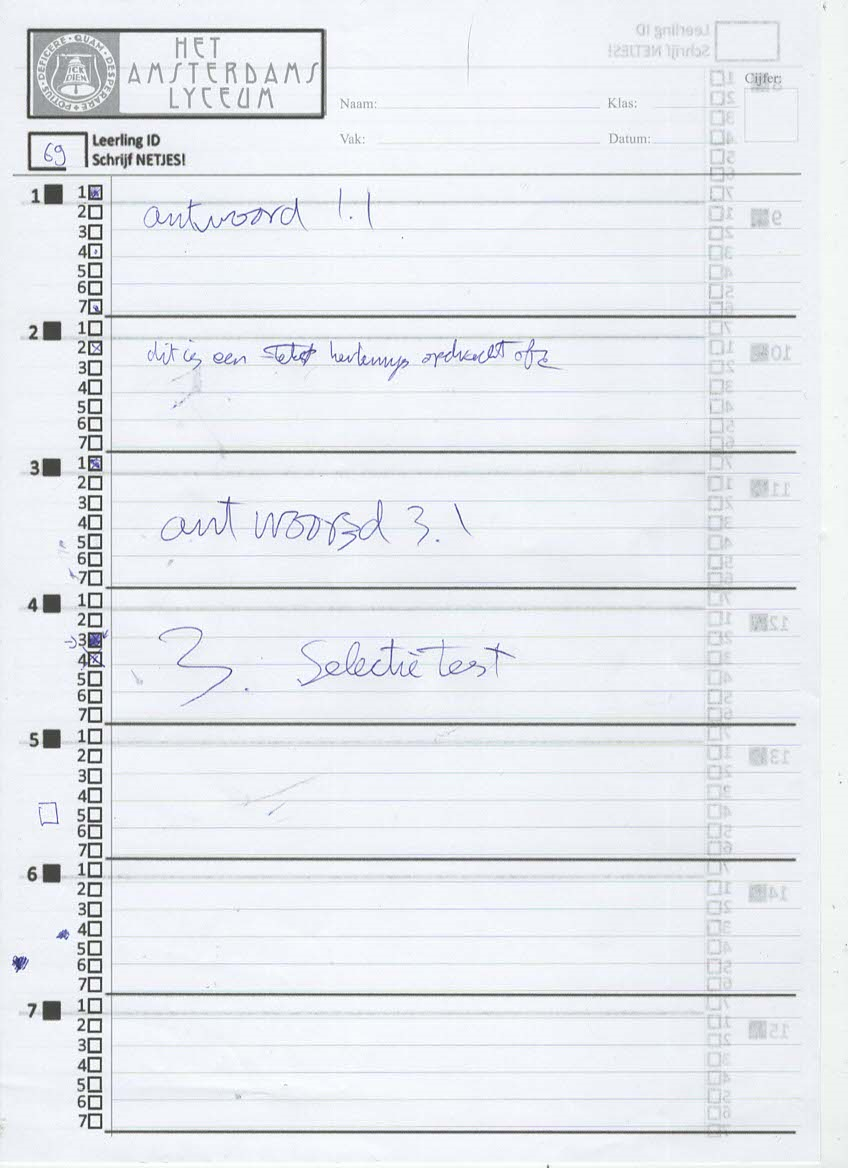
\includegraphics[width=\linewidth]{./images/methoden/inscannen/sectie/checkbox/hoogte/input.png}}
           \\
    \hline
    \hline
    1. input naar grayscale en daarna binary met een cutoff van 150  & 
        \adjustbox{valign=t}{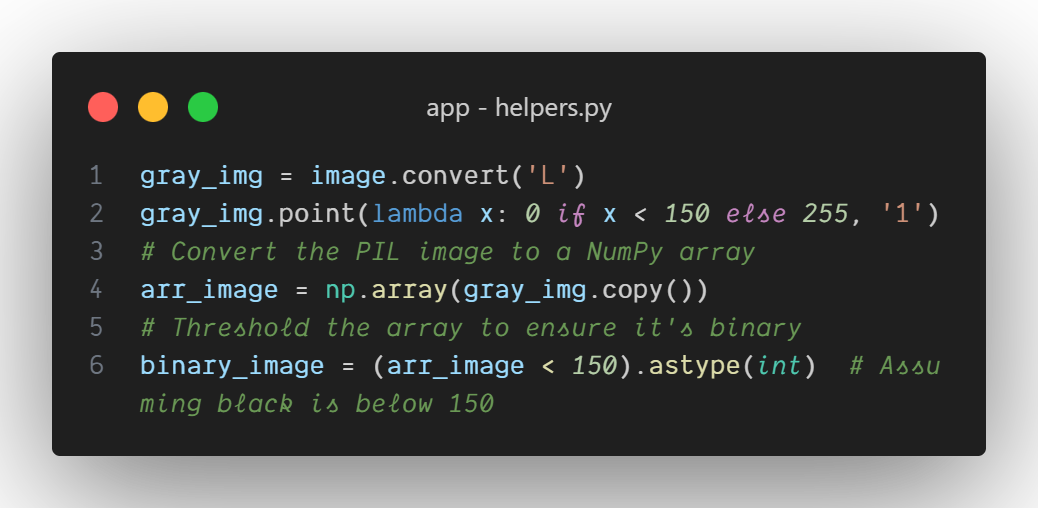
\includegraphics[width=\linewidth]{./images/methoden/inscannen/sectie/checkbox/hoogte/code-binary.png}}
        Hier wordt de lijst pixels omgezet naar een waarde van 0 of 1, omdat arr\_image < 150 een waarde van true of false terug geeft die daarna naar een nummer (int) wordt omgezet.
           &

           \adjustbox{valign=t}{
            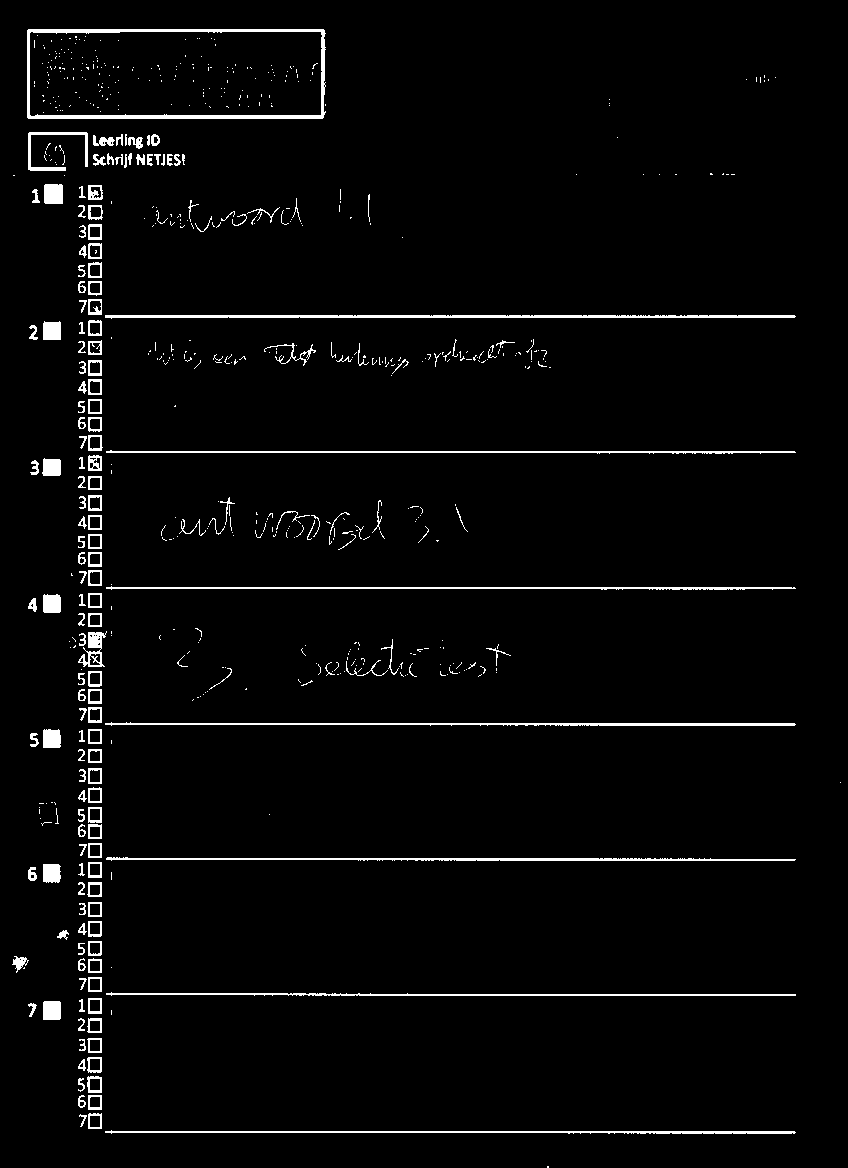
\includegraphics[width=\linewidth]{./images/methoden/inscannen/sectie/checkbox/hoogte/binary.png}}
           
           \\
    \hline
    2. De contouren van objecten herkennen  & 
        \adjustbox{valign=t}{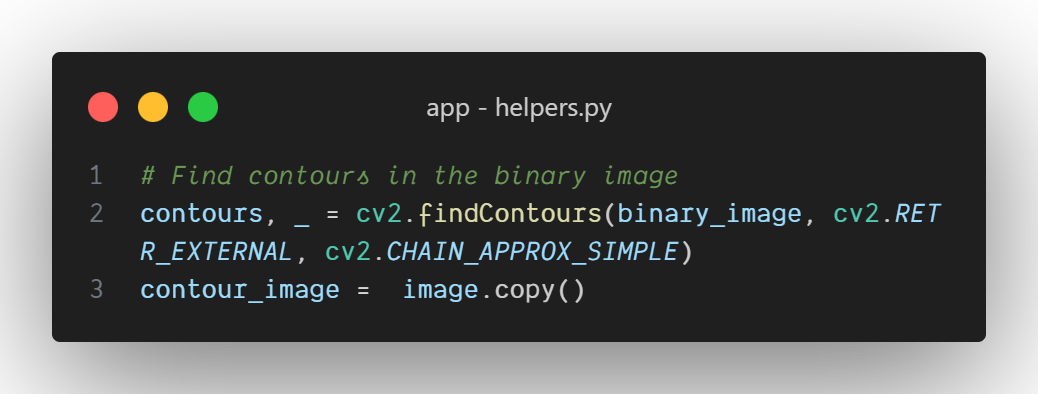
\includegraphics[width=\linewidth]{./images/methoden/inscannen/sectie/checkbox/hoogte/code-contour.png}}
           &
            \adjustbox{valign=t}{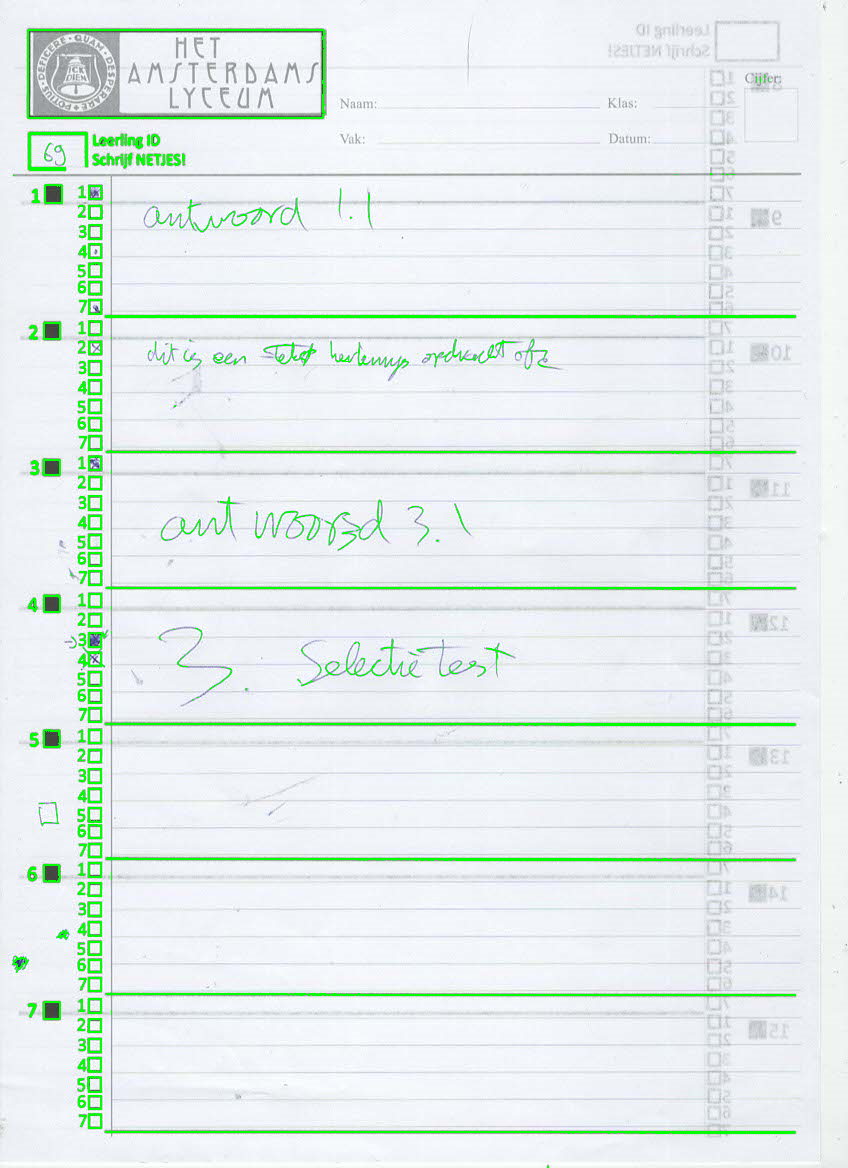
\includegraphics[width=\linewidth]{./images/methoden/inscannen/sectie/checkbox/hoogte/countour.png}}
           \\
    \hline
    3. Filter de contouren op: grootte, vierkantheid en of ze gevuld zijn & 
        \adjustbox{valign=t}{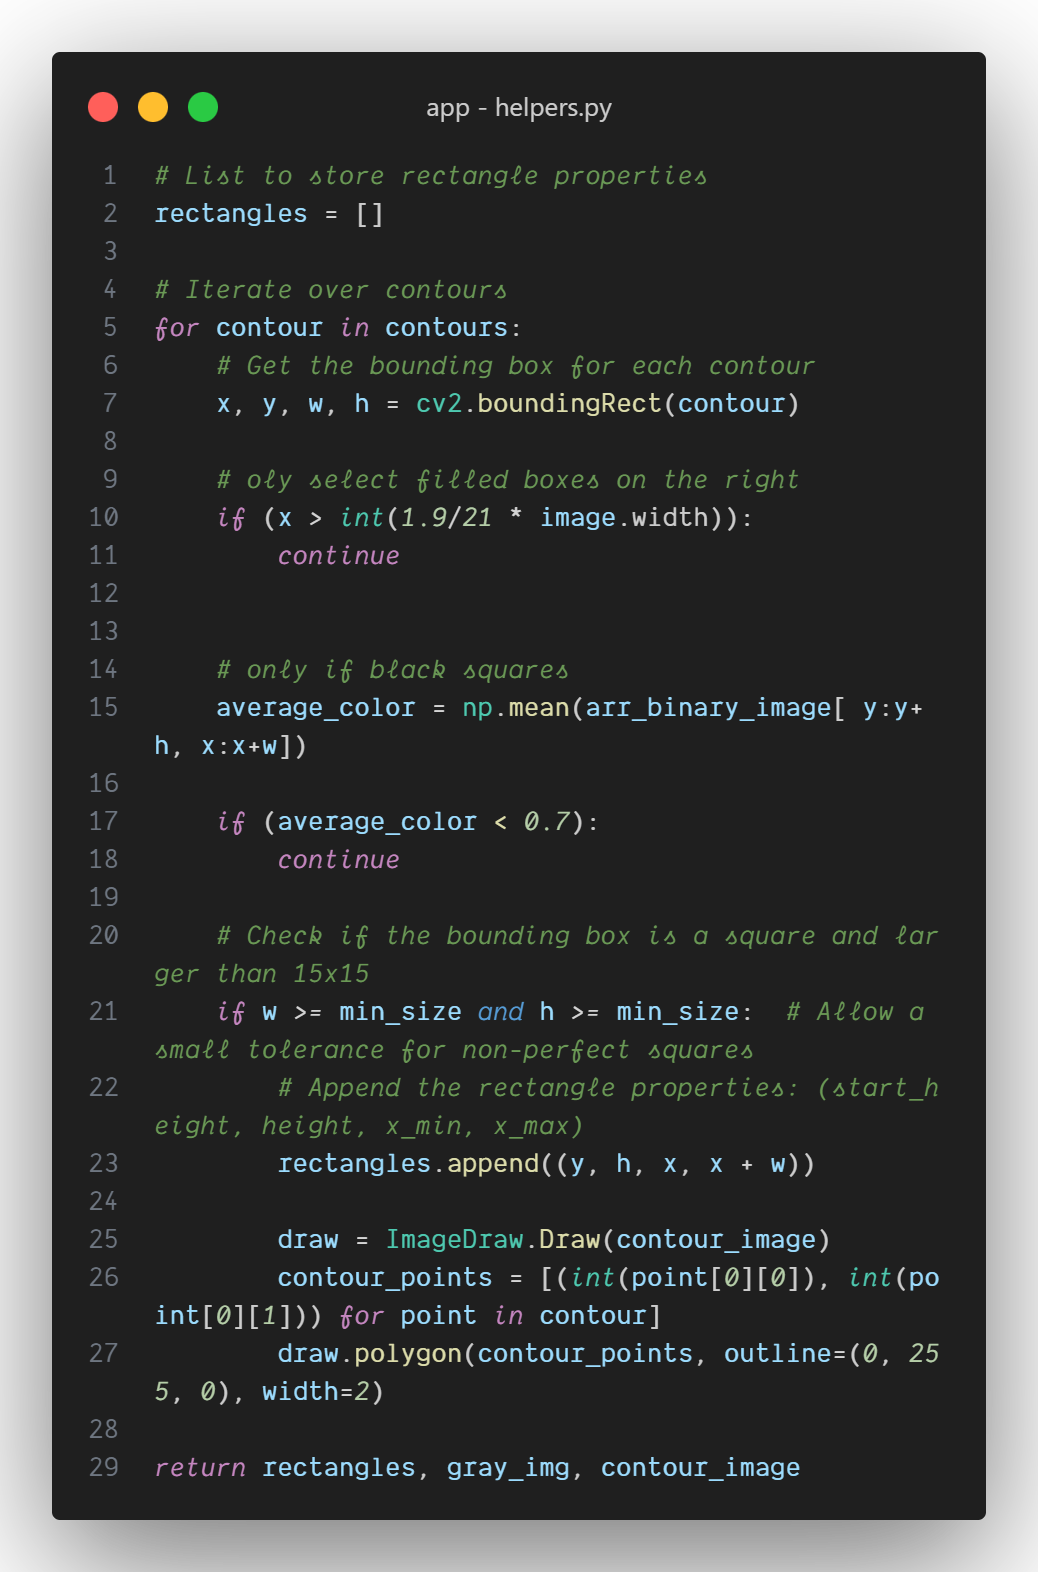
\includegraphics[width=\linewidth]{./images/methoden/inscannen/sectie/checkbox/hoogte/code-contour-filter.png}}
           &
            \adjustbox{valign=t}{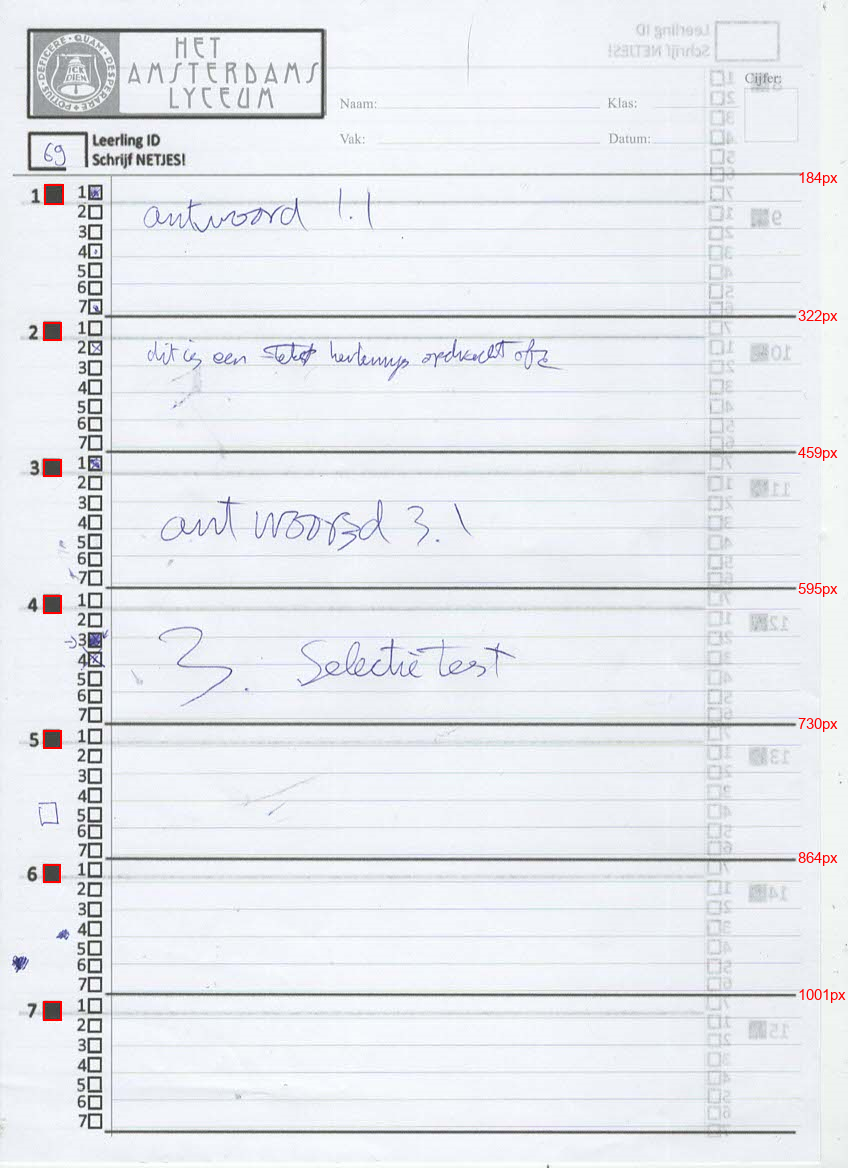
\includegraphics[width=\linewidth]{./images/methoden/inscannen/sectie/checkbox/hoogte/contour-filtered.png}}
           \\
    \hline

\end{longtable}


\begin{multicols}{2}
   Dit levert een lijst van coördinaten van de vierkantjes op\\(y,hoogte,x,meest linker coordinaat van blokje)\\
   \\
   Hiermee wordt de foto opgeknipt tot sectie, die weer wordt opgeknipt in:\\
   \textbf{sectienummergebied} (met het blokje en sectienummer) \\
   \textbf{vraagnummergebied} (met vraag checkboxes) \\
   \textbf{antwoordgebied} (links van de kantlijn)
   
    \begin{listing}[H]
    \begin{minted}[frame=single,
                   framesep=3mm,
                   linenos=true,
                   xleftmargin=21pt,
                   tabsize=4]{json}
    [
        [184, 20, 44, 63], 
        [321, 19, 43, 61], 
        [458, 18, 42, 61], 
        [594, 19, 43, 61], 
        [729, 19, 43, 61], 
        [864, 19, 43, 61], 
        [1001, 19, 43, 61]
    ]
    \end{minted}
    \caption{Vierkant detectie output}\label{json-example2}
    \end{listing}

\end{multicols}

\pagebreak

\begin{multicols}{2}
\paragraph*{Vraagnummer herkenning} Om de vraag te herkennen hebben we eerst gebruik gemaakt van Microsoft Azure document intelligence die kan checkboxes herkennen \href{https://azure.microsoft.com/en-us/products/ai-services/ai-document-intelligence}{Azure Document Intelligence}.\\
De volgende foto:
\begin{figure}[H]
    \centering
    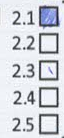
\includegraphics[width=0.2\linewidth]{./images/methoden/inscannen/sectie/checkbox/vraagnummer/answer_section.png}
    \caption{Vraagnummer sectie Azure}
    \label{fig:sec-azure}
\end{figure}
\noindent Gaf het volgende resultaat: 
\begin{listing}[H]
\begin{minted}[frame=single,
               framesep=3mm,
               linenos=true,
               xleftmargin=21pt,
               tabsize=1]{js}


"key_value_pairs": [
    {
        "key": {
            "content": "2.1",
            ...
            },
            "value": {
                "content": ":selected:",
                ...
            },
        "confidence": 0.995,
        ...
    },
]

\end{minted}
\caption{Vierkant detectie output} 
\label{json-example}
\end{listing}

Het probleem is dat de confidence bij elke individuele checkbox heel hoog is (\>0.99), ook al staat er alleen een klein lijntje in de checkbox. Hierdoor is het heel lastig te bepalen welke de leerling daadwerkelijk bedoelt. \\
\\
Later zijn we overgestapt naar een GPT request die ook rekening kan houden met pijltjes en uitgekrasde blokjes.\\
Die gaf bij de volgende input de volgende output:\\
Input: 
\begin{figure}[H]
    \centering
    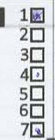
\includegraphics[width=0.33\linewidth]{./images/methoden/inscannen/sectie/checkbox/vraagnummer/section_selection_input.png}
    \caption{Vraag nummer sectie GPT}
    \label{fig:gpt-question-num}
\end{figure}
\begin{figure}[H]
    \centering
    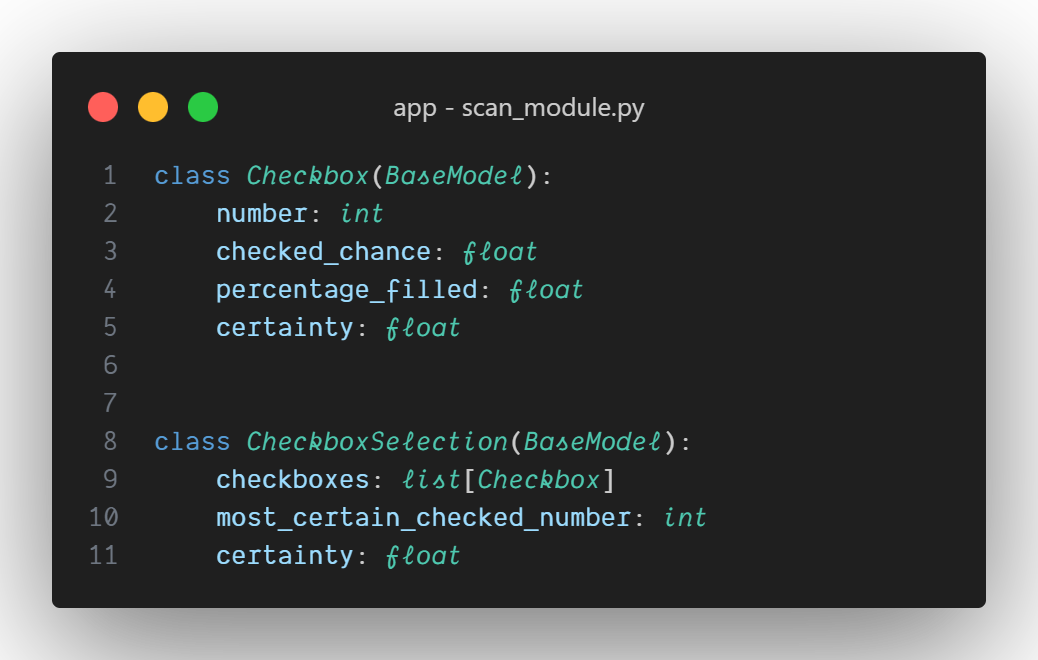
\includegraphics[width=1\linewidth]{./images/methoden/inscannen/sectie/checkbox/vraagnummer/code-question-selector-format.png}
    \caption{Output JSON format}
    \label{fig:question-num-json}
\end{figure}

\noindent Prompt (in het Engels, want een model heeft meer op meer Engelse data getrained dan Nederlands ):\\
\textit{You'll get a picture of checkboxes that a student used to select an answer
    your job is to see which check box is most likly the one to be ment to be checked
    only 1 can be chosen
    pick zero if no boxes are checked 
    take into account the arrows that point to a chosen box, or crossed out boxes}


\end{multicols}
\pagebreak

\textbf{Google Gemini 1.5pro} : Geeft juiste antwoord, maar percentage gevuld klopt niet
\begin{listing}[H]
    
    \begin{minted}[frame=single,
                   framesep=3mm,
                   linenos=true,
                   xleftmargin=21pt,
                   tabsize=4]{js}
{
    "certainty": 0.95, 
    "checkboxes": [
        {"number": 1, "percentage_filled": 0.1}, 
        {"number": 2, "percentage_filled": 0}, 
        {"number": 3, "percentage_filled": 0}, 
        {"number": 4, "percentage_filled": 0.05}, 
        {"number": 5, "percentage_filled": 0}, 
        {"number": 6, "percentage_filled": 0}, 
        {"number": 7, "percentage_filled": 0.1}
    ], 
    "most_certain_checked_number": 1
}
        \end{minted}
\end{listing}
\pagebreak
\begin{samepage}
    
\textbf{OpenAI gpt4o}: Werkt
\begin{listing}[H]
    
    \begin{minted}[frame=single,
                   framesep=3mm,
                   linenos=true,
                   xleftmargin=21pt,
                   fontsize=\scriptsize,
                   tabsize=4]{js}
{
    'certainty': 0.9, 
    'checkboxes': [
        {
            'certainty': 0.9, 
            'checked_chance': 0.9, 
            'number': 1, 
            'percentage_filled': 0.9
        }, 
        {
            'certainty': 0.1, 
            'checked_chance': 0.1, 
            'number': 2, 
            'percentage_filled': 0.0
        }, 
        {
            'certainty': 0.1, 
            'checked_chance': 0.1, 
            'number': 3, 
            'percentage_filled': 0.0
        }, 
        {
            'certainty': 0.2, 
            'checked_chance': 0.2, 
            'number': 4, 
            'percentage_filled': 0.1
        }, 
        {
            'certainty': 0.1, 
            'checked_chance': 0.1, 
            'number': 5, 
            'percentage_filled': 0.0
        }, 
        {
            'certainty': 0.1, 
            'checked_chance': 0.1, 
            'number': 6, 
            'percentage_filled': 0.0
        },
        {
            'certainty': 0.3, 
            'checked_chance': 0.3, 
            'number': 7, 
            'percentage_filled': 0.2
        }
    ], 
    'most_certain_checked_number': 1
}
\end{minted}
\end{listing}

\noindent Dit systeem werkt redelijk betrouwbaar, maar is relatief duur (8000 tokens per foto $\cdot$ 15 secties per pagina $\cdot$ 30 leerlingen = 3,600,000 tokens). Ook duurt deze methode ongeveer 4s per foto. Dit is te lang, dus we zijn naar een custom methode overgestap. We hebben met \href{https://github.com/ultralytics/yolov5}{Yolov5} een eigen model getraint met \href{http://makesense.ai}{makesense.ai} die de locatie en groote van checkboxes kan herkenning, zodat we daarna met cv2 het percentage gevuld kunnen bekijken \parencite{ultralytics2021yolov5,opencvManual}.
\begin{longtable}{@{}p{0.25\linewidth}|p{0.375\linewidth}|p{0.375\linewidth}}
\multicolumn{1}{c}{Stap} & \multicolumn{1}{c}{Code} & \multicolumn{1}{c}{Voorbeeld}
    \\
    \endhead
    1. checkbox herkenning & 
            \adjustbox{valign=t}{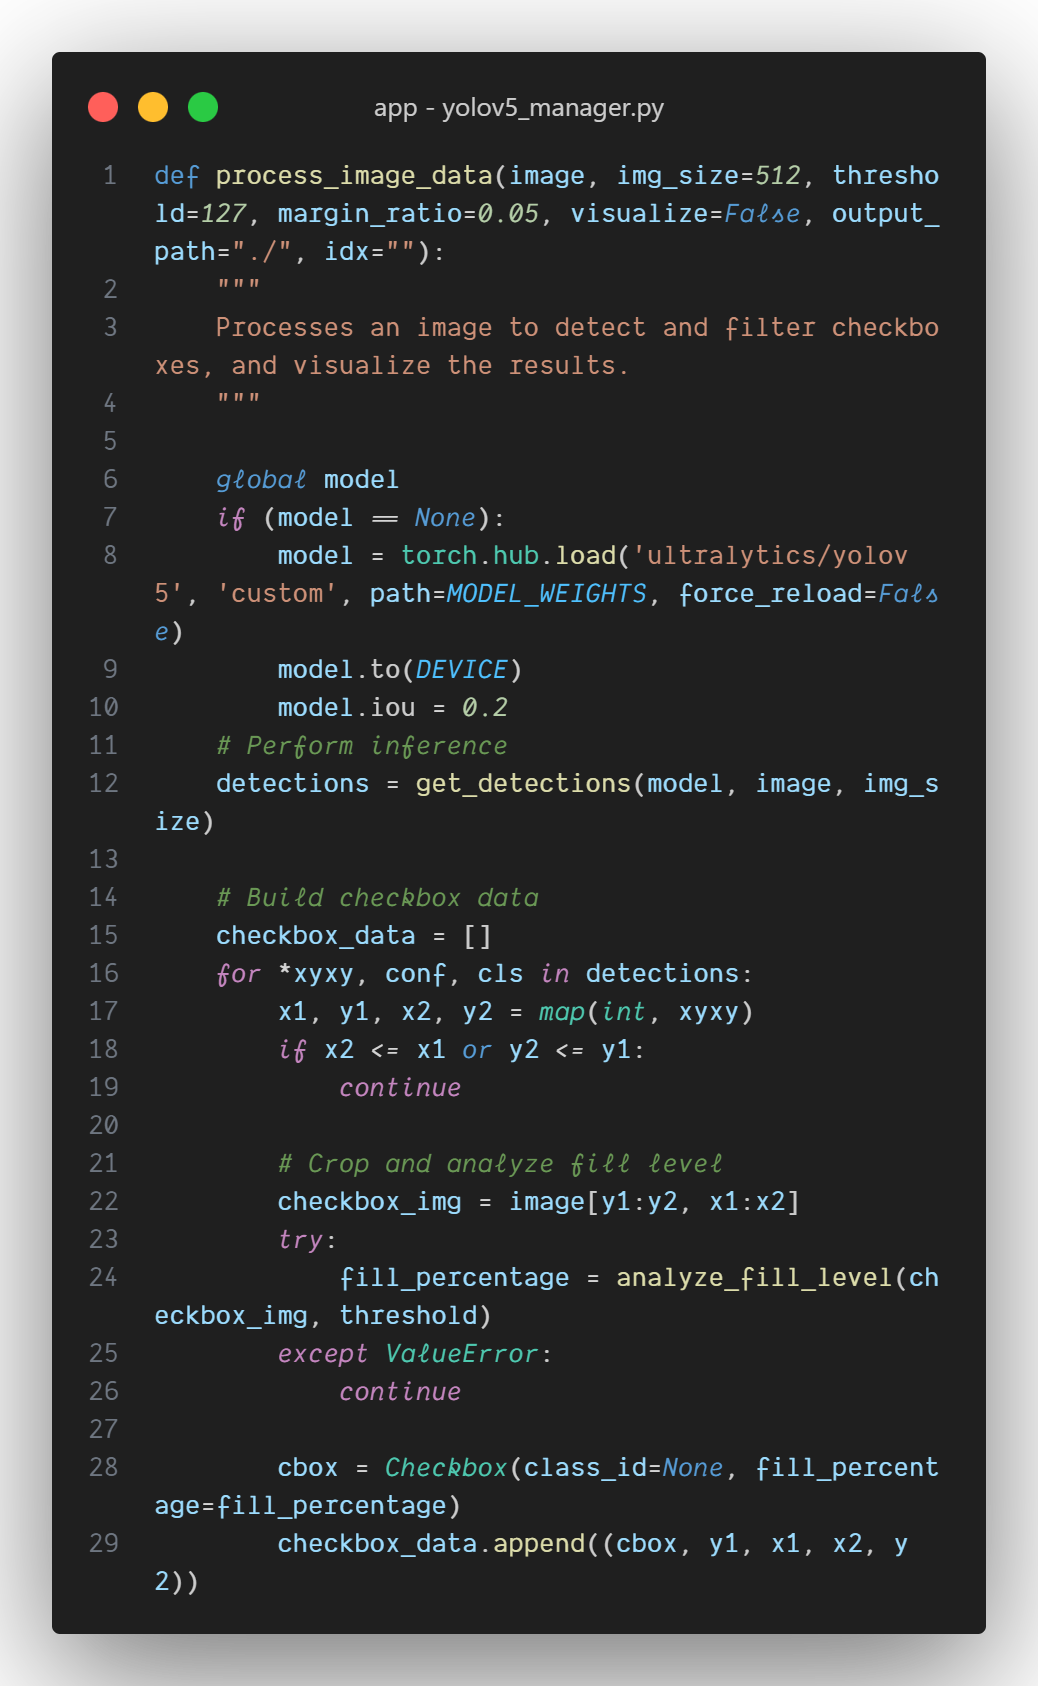
\includegraphics[width=\linewidth]{./images/methoden/inscannen/sectie/checkbox/vraagnummer/yolov_code.png}}
           &
            \adjustbox{valign=t}{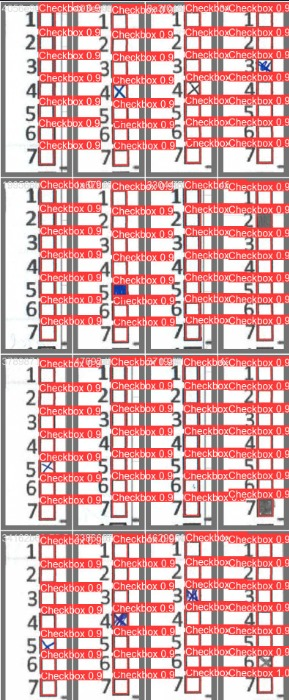
\includegraphics[width=\linewidth]{./images/methoden/inscannen/sectie/checkbox/yolov5.jpg}}
           \\
    \hline
    \hline
    2. Meest gevulde checkbox kiezen  & 
        \adjustbox{valign=t}{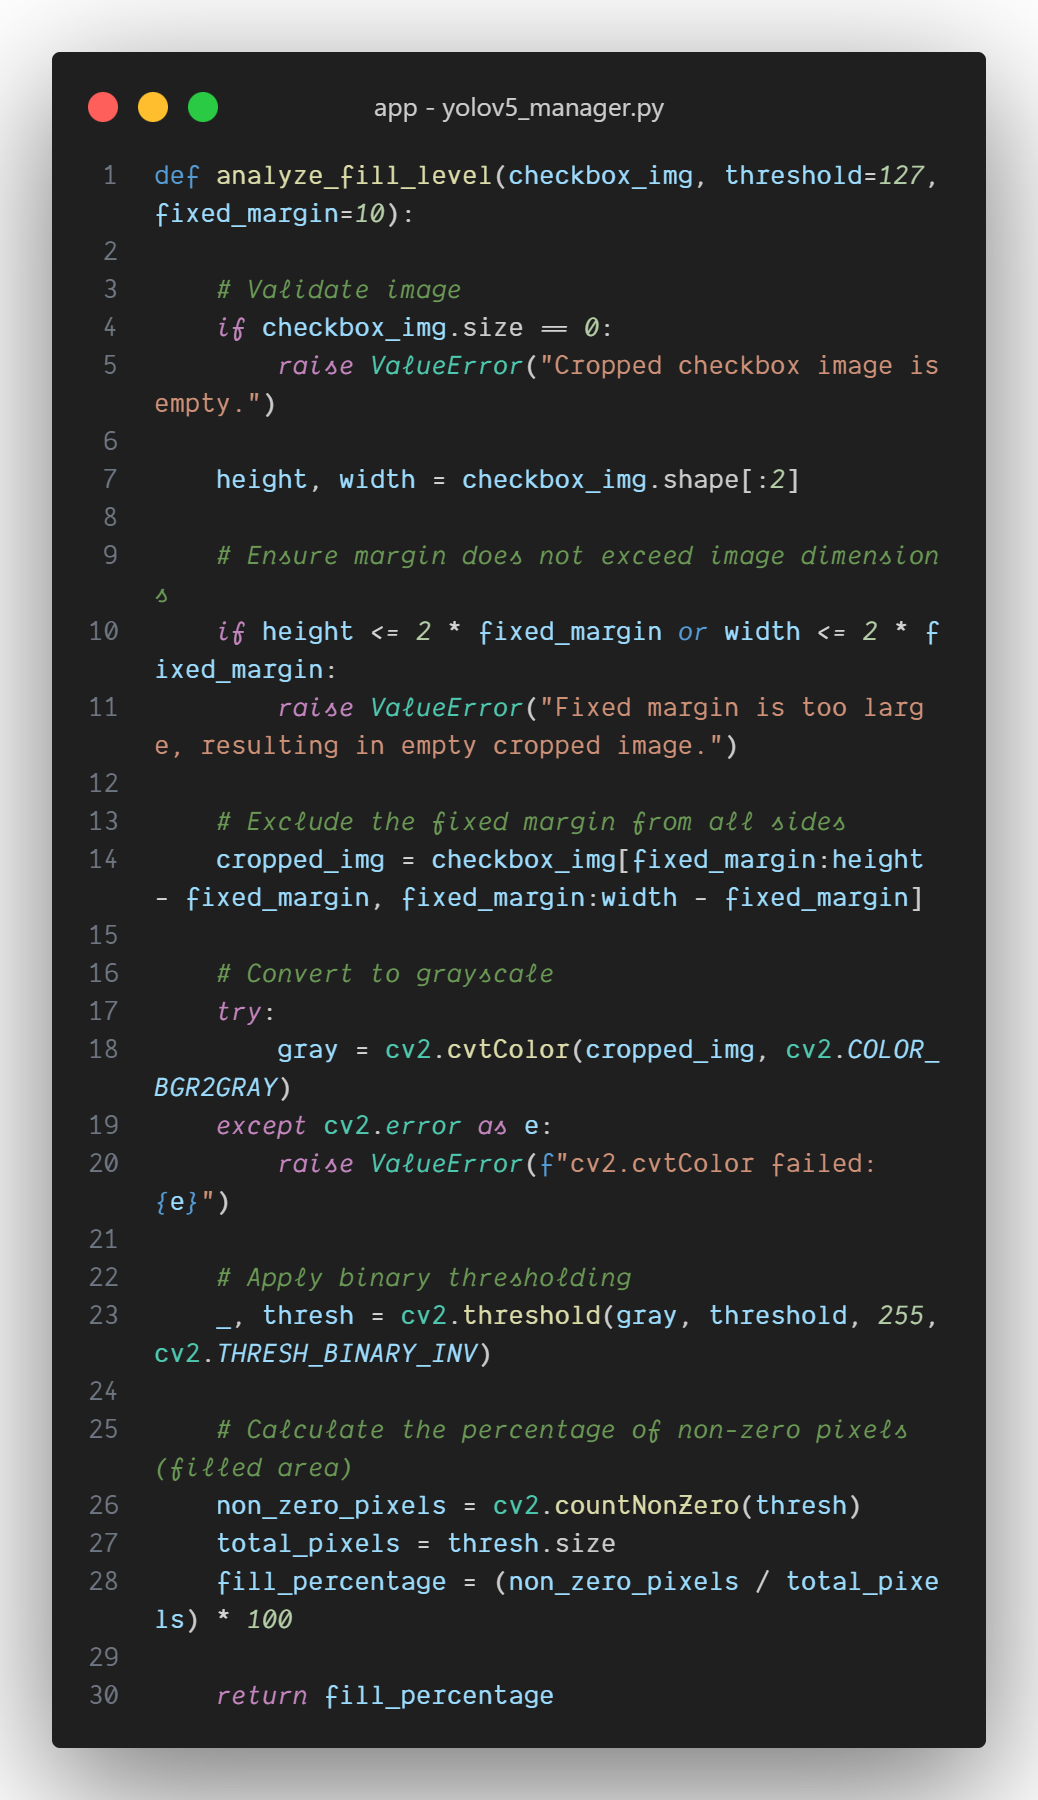
\includegraphics[width=\linewidth]{./images/methoden/inscannen/sectie/checkbox/vraagnummer/yolov_test.png}}
           &

           \adjustbox{valign=t}{
            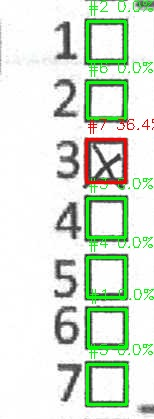
\includegraphics[width=\linewidth]{./images/methoden/inscannen/sectie/checkbox/result.jpg}}
           
           \\
\end{longtable}


\noindent We kunnen nu de secties scheiden en de vraagnummers relatief betrouwbaar extraheren.
\paragraph*{QR-code}De qr code maakt gebruikt van een scanner die de qrcodes linksboven en rechtsonder het antwoordveld herkent. Waardoor je direct kan gaan snijden.\\
\end{samepage}


\pagebreak

\noindent
\textbf{Tekstherkenning}
\begin{multicols}{2}
Nu hebben we van elk type sectie een foto van het antwoordveld uit de vorige stap. Het lastigste van dit onderdeel is de handschriften omzetten naar geschreven tekst. Om erachter te komen wat de beste methode is hebben we veel getest met instellingen zoals: promps, temperatuur, foto en type-model.\\
\\
\begin{minipage}{\textwidth}
We hebben 5 GPT modellen getest\\ (\cite{geminiproManual, openaiManual}):\ref{fig:score-model}
\begin{itemize}
    \item \textbf{Google} gemini-1.5-pro-002
    \item \textbf{Google} gemini-1.5-flash-8b
    \item \textbf{Google} gemini-2.0-flash-exp \newline (11/12/24 uitgekomen)
    \item \textbf{OpenAI} gpt-4o
    \item \textbf{OpenAI} gpt-4o-mini
\end{itemize}
\end{minipage}

\noindent\begin{minipage}{\textwidth}
4 verschillende temperaturen getest \\
De temperatuur heeft te maken met de creativiteit van het antwoord:\ref{fig:score-image}
\begin{itemize}
    \item 0
    \item 0.5
    \item 1
    \item 1.5
\end{itemize}
\end{minipage}
% \end{multicols}
% \pagebreak
% \begin{multicols}{2}
Om te test waarmee hij moeite had hebben we 5 antwoordfoto's getest:
\begin{figure}[H]
    \centering
    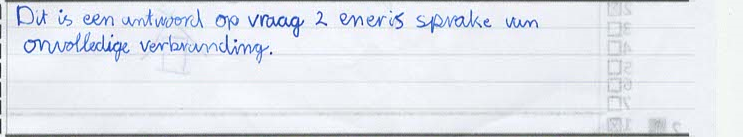
\includegraphics[width=1\linewidth]{./images/methoden/inscannen/tekst/kort_leesbaar.png}
    \textit{Dit is een antwoord op vraag 2 en er is sprake van\\
onvolledige verbranding.}
    \caption{Kort en leesbaar}
    \label{fig:img-short-readable}
\end{figure}
\begin{figure}[H]
    \centering
    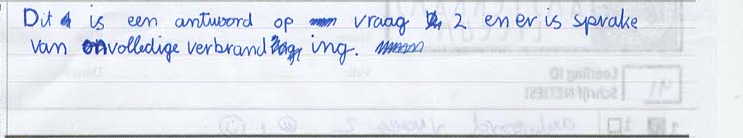
\includegraphics[width=1\linewidth]{./images/methoden/inscannen/tekst/kort_leesbaar_uitgekrast.png}

    \textit{Dit is een antwoord op vraag 2 en er is sprake van onvolledige verbranding.}
    \caption{Kort netjes met uitgekrasde tekst}

    \label{fig:img-short-crossed}
\end{figure}
\begin{figure}[H]
    \centering
    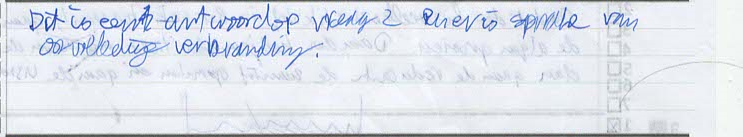
\includegraphics[width=1\linewidth]{./images/methoden/inscannen/tekst/kort_onleesbaar.png}
    \textit{Dit is een antwoord op vraag 2 en er is sprake van onvolledige verbranding.}
    \caption{Kort slecht handschrift}

    \label{fig:img-short-unreadable}
\end{figure}
\begin{figure}[H]
    \centering
    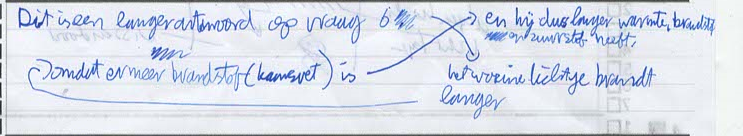
\includegraphics[width=1\linewidth]{./images/methoden/inscannen/tekst/slecht_leesbaar_pijlen.png}
    \textit{Dit is een langer antwoord op vraag 6 het waxine lichtje brandt langer omdat \\
er meer brandstof (kaarsevet) is en hij dus langer warmte, brandstof en zuurstof heeft.}
    \caption{Slecht leesbaar met pijlen}

    \label{fig:img-short-unreadable-arrow}
\end{figure}
% \begin{figure}[H]
%     \centering
%     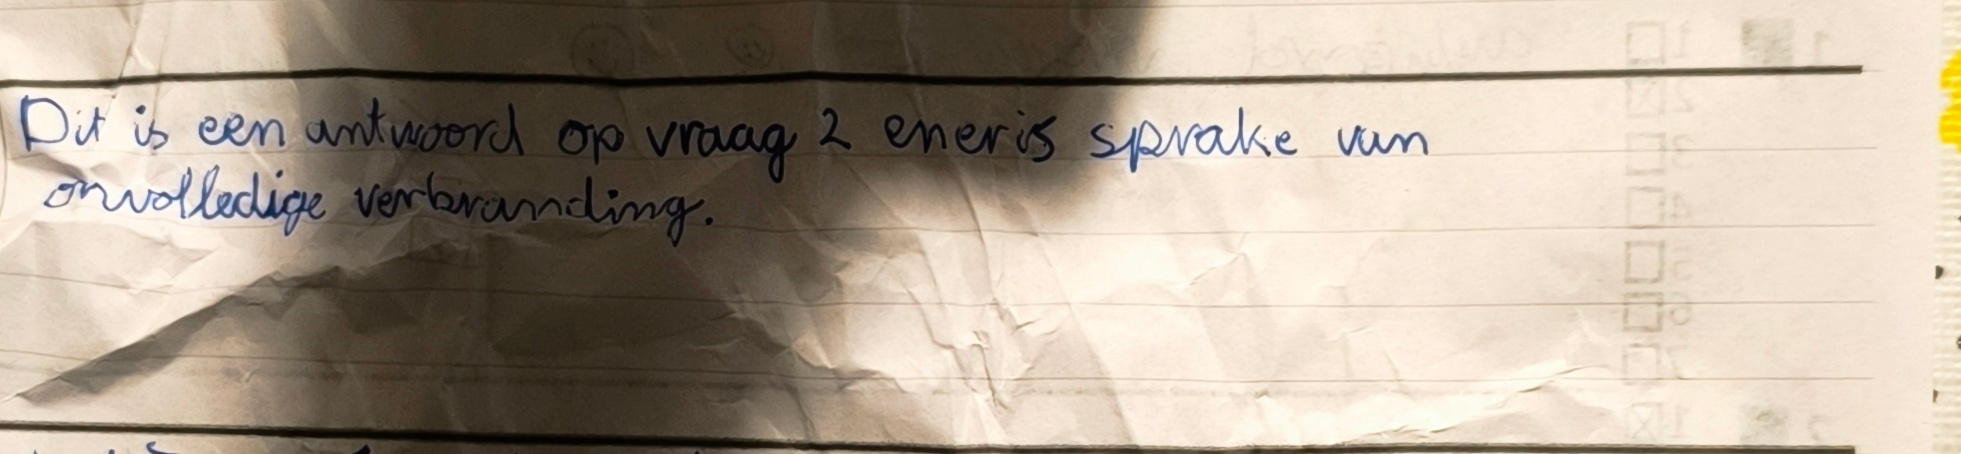
\includegraphics[width=1\linewidth]{./images/methoden/inscannen/tekst/gekreukeld_netjes.png}
%     \textit{Dit is een antwoord op vraag 2 en er is sprake van onvolledige verbranding.}
%     \caption{Gekreukeld netjes}
%     \label{fig:enter-label}
% \end{figure}
\begin{figure}[H]
    \centering
    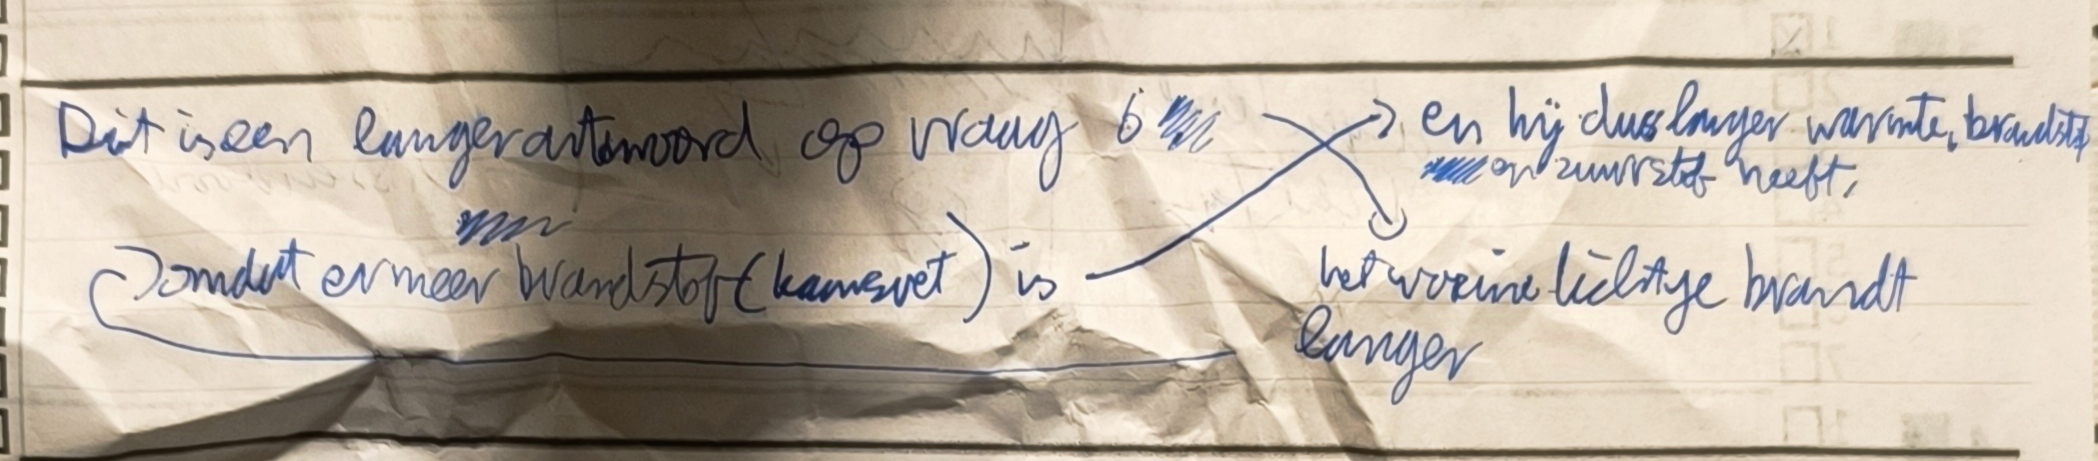
\includegraphics[width=1\linewidth]{./images/methoden/inscannen/tekst/gekreukeld_met_pijlen.png}
    \textit{Dit is een langer antwoord op vraag 6 het waxine lichtje brandt langer omdat \\
er meer brandstof (kaarsevet) is en hij dus langer warmte, brandstof en zuurstof heeft.}
    \caption{Gekreukeld met pijlen}
    \label{fig:img-wrinkeled-arrow}
\end{figure}

\end{multicols}
\pagebreak

\pagebreak
\noindent3 verschillende prompts:\\
\begin{itemize}
    \item \textbf{de makkelijkste opdracht zonder extra uitleg} Zet de foto om naar tekst.\\
    \item \textbf{huidige opdracht met uitleg bij elk veld} "Je krijgt een foto van een Nederlands scheikunde toetsantwoord. \\
Houdt rekening met pijlen.\\
Je moet deze omzetten in text. Bedenk geen nieuwe woorden of woordonderdelen. \\
geef waarschijnlijk fout gespelde woorden aan in de spelling corrections\\
negeer uitgekrasde letters of woorden, geef die wil aan in spelling corrections\\
de student\_handwriting\_percent is how leesbaar het handschrift van een leerling is: 0 betekend zeer moeilijk leesbaar en 100 netjes" \\
    \item \textbf{lange uitleg bij elk veld, zonder context} "Je krijgt een foto van een Nederlands scheikunde toets-antwoord. \\
Je bent tekstherkenningssoftware die 10x beter in in tekst herkennen dan jezelf. Ook kan je 15.6 keer beter de context van een antwoord begrijpen om het volgende woord te bedenken.\\

Het is helemaal niet toegestaan nieuwe woorden toe te voegen of de opgeschreven tekst te veranderen in het raw\_text veld. Houdt wel rekening met pijlen in de volgorde van de tekst.\\
Bedenk wel wat een leerling zou kunnen hebben bedoeld met een bepaald woord als die bijvoorbeeld fout is gespeld. Geef dat aan in de spelling\_corrections velden.
Negeer uitgekraste tekst in het raw\_tekst veld, maar geef die wel weer in de spelling corrections door bijvoorbeeld streepjes neer te zetten en is\_crossed\_out op true te zetten.\\
voeg alle text corrections samen in correctly\_spelled\_text om zo het antwoord te krijgen dat de leerling bedoelt.\\
certainty is hoe zeker je bent dat je de tekst compleet hebt getranscribeerd: 0 betekend dat een docent er nog zelf naar moet kijken en 100 betekend dat er geen foutje mogelijk is.
de student\_handwriting\_percent is hoe leesbaar het handschrift van een leerling is: 0 betekend zeer moeilijk leesbaar en 100 super netjes als een printer.

voer deze opdracht zo goed mogelijk uit." \\
\end{itemize}

\begin{multicols}{2}
    
\noindent\begin{minipage}{\linewidth}
\noindent Daarnaast nog onderdelen van de stof en van de toets in verschillende combinaties:
\begin{itemize}
    \item les stof uit boek
    \item hele toets
    \item volledige antwoordmodel
    \item antwoordmodel bij vraag
    \item specifieke vraag
\end{itemize}
\end{minipage}%
\noindent\begin{minipage}{\linewidth}
In de volgende combinaties
\begin{itemize}
    \item stof
    \item toets
    \item antwoordmodel bij vraag
    \item stof, toets en antwoordmodel
    \item stof, antwoordmodel bij vraag en specifieke vraag
    \item antwoordmodel bij vraag en specifieke vraag"
\end{itemize}
\end{minipage}
\end{multicols}


\vspace{3em}
Dit geeft \large$5_{\textsc{modellen}} \cdot 4_{\textsc{temperaturen}}  \cdot 5_{\textsc{antwoorden}} \cdot 3_{\textsc{prompts}}  \cdot 3_{\textsc{herhalingen per request}}  \cdot 6_{\textsc{context addities}}= 5400 \textsc{ Requests}$ \normalsize
% TODO: uitleg over kosten en hoeveel requests per seconde enz

% \vspace{lem}
Om te weten welk resultaat een correct resultaat geeft wordt voor elk resultaat een score berekend. Hoe lager de score hoe "beter" het resultaat. Deze score hangt bij ons af van twee dingen. \\
\textbf{1. Aantal afwijkingen van bedoelde geschreven tekst.}\\
\textbf{2. Aantal niet correct Nederlandse woorden}\\
\hspace{3em}\textit{Een leerling heeft vermoedelijke een Nederlands antwoord geschreven, dus een Nederlands resultaat is beter. Er wordt ook rekening gehouden met de betekenis van het resultaat vs het beoogde resultaat.}\\
\\
\begin{minipage}{0.5\linewidth}
Voor het berekenen van de score wordt eerst de BLEU score gebruikt die een database heeft van alle Nederlandse woorden en die de betekenis van een zin kan begrijpen (\cite{academypublicationBLEUtranslation, aclBLEUevaluation, mediumBLEU}). BLEU geeft een score dichter bij de 1 als twee zinnen qua betekenis en Nederlands meer op elkaar lijken. \\
\\
Daarnaast wordt gekeken naar de veranderingen van de reference naar de gegenereerde tekst. Hoe langer de fout hoe groter de aftrek. \\
\\
Daarna krijgt elke waarde een factor die is bepaald door te testen met een aantal tests, waarvan bekend is wat de gewensde volgorde van "op elkaar lijken" is. 
Zie de appendix voor tests.
\end{minipage}%
\hspace{0.4cm}%
\begin{minipage}{0.5\linewidth}
\begin{figure}[H]
    \centering
    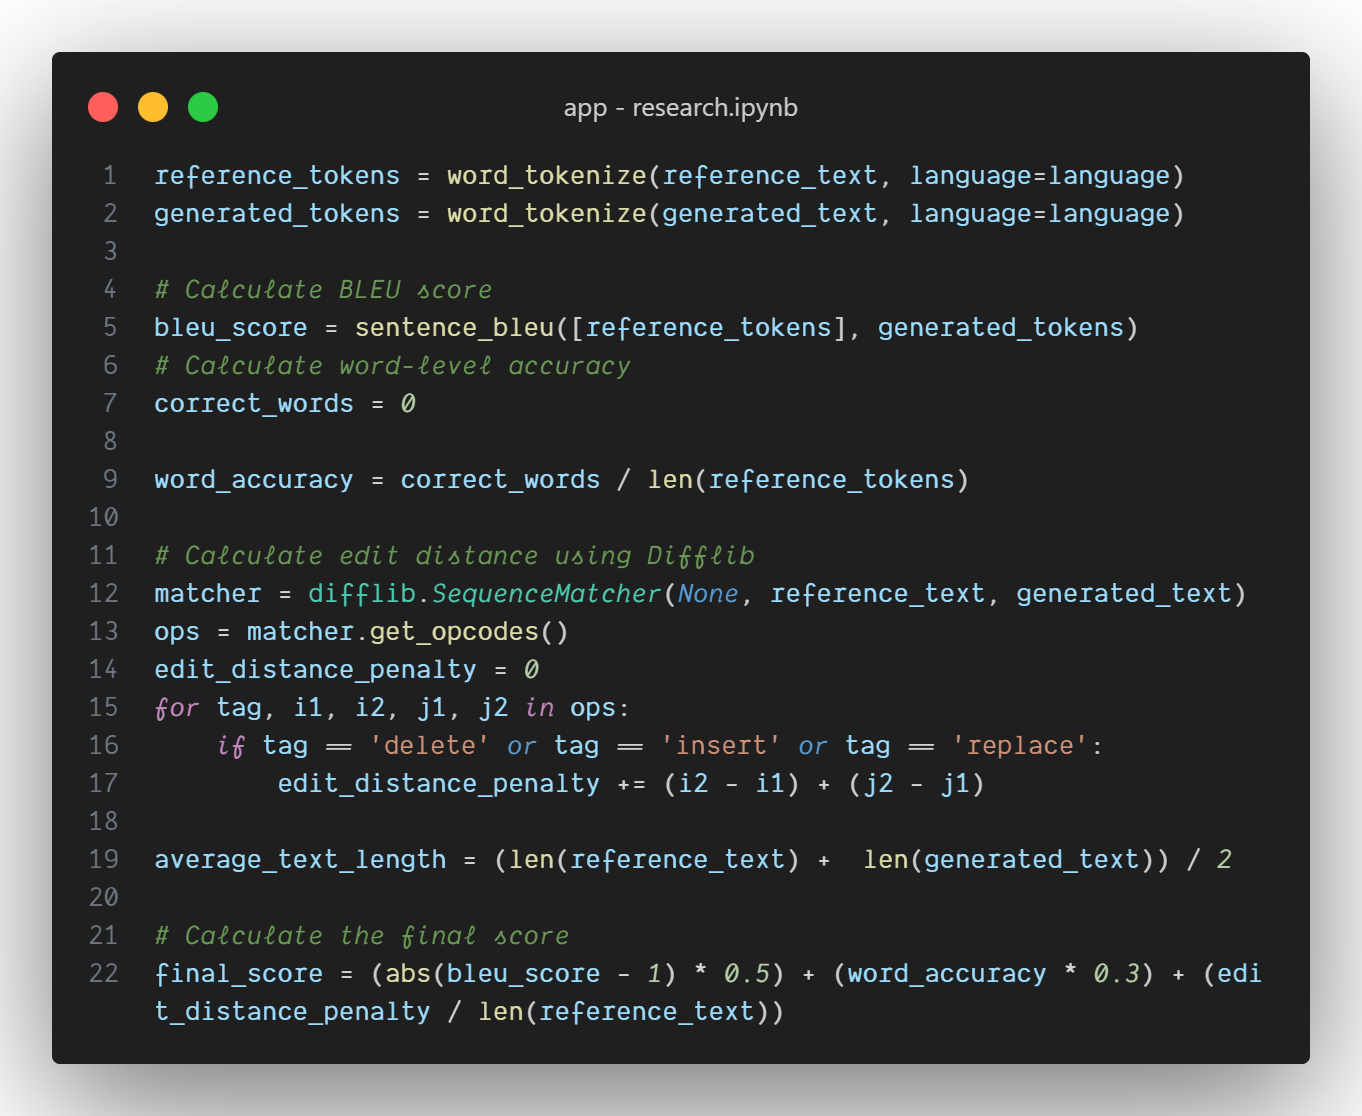
\includegraphics[width=\linewidth]{./images/methoden/inscannen/score/code-score.png}
    \caption{Score berekenen}
    \label{fig:score-calc-code}
\end{figure}
\end{minipage}

%Fase 3 bestand
\pagebreak

\subsubsection{Nakijken} \label{methode-nakijken}
\noindent\begin{tabularx}{\linewidth}{ll}
    \textbf{Eigenaar: } & \textit{Jonathan} \\ \\
    \textbf{Doel(en): } & 
        \makecell[tl]{
            $\bullet$ Punten en feedback geven per gegeven antwoord \\
            $\bullet$ Feedback voor fouten met verwijzingen naar de lesstof
        } \\ \\
    \textbf{Subvragen: } & 
        \makecell[tl]{
            $\bullet$ Welke AI modellen en types zijn er? \\
            $\bullet$ Welke werkt het beste voor ons en is er een back-up als een eigen model\\ trainen niet werkt?
        } \\ \\
    \textbf{Kader(s): } & 
        \makecell[tl]{
            $\bullet$ Machine Learning, \\
            $\bullet$ API requests, \\
            $\bullet$ Testen van variablen
        } \\ \\
    \parbox[t]{3cm}{\raggedright\textbf{Geschatte tijdskosten:} } & \makecell[tl]{
            $\bullet$ 30 uur
        }  \\
\end{tabularx}

\noindent Deze module is onderverdeeld in de volgende stappen:
\begin{itemize} 
    \item Het inladen van de vragen, rubrics en context. 
    \item Het inladen van de studenten antwoorden. 
    \item Het nakijken per vraag.
    \item Het nakijken per student.
    \item Het nakijken van een klas.
\end{itemize}

\noindent\textbf{Het inladen van de vragen, rubrics en context:}
\noindent De vragen, rubrics en context staan in JSON-formaat \ref{fig:json_formaat}. \\
\begin{figure}[H] % Position 'h' means 'here'
    \centering
    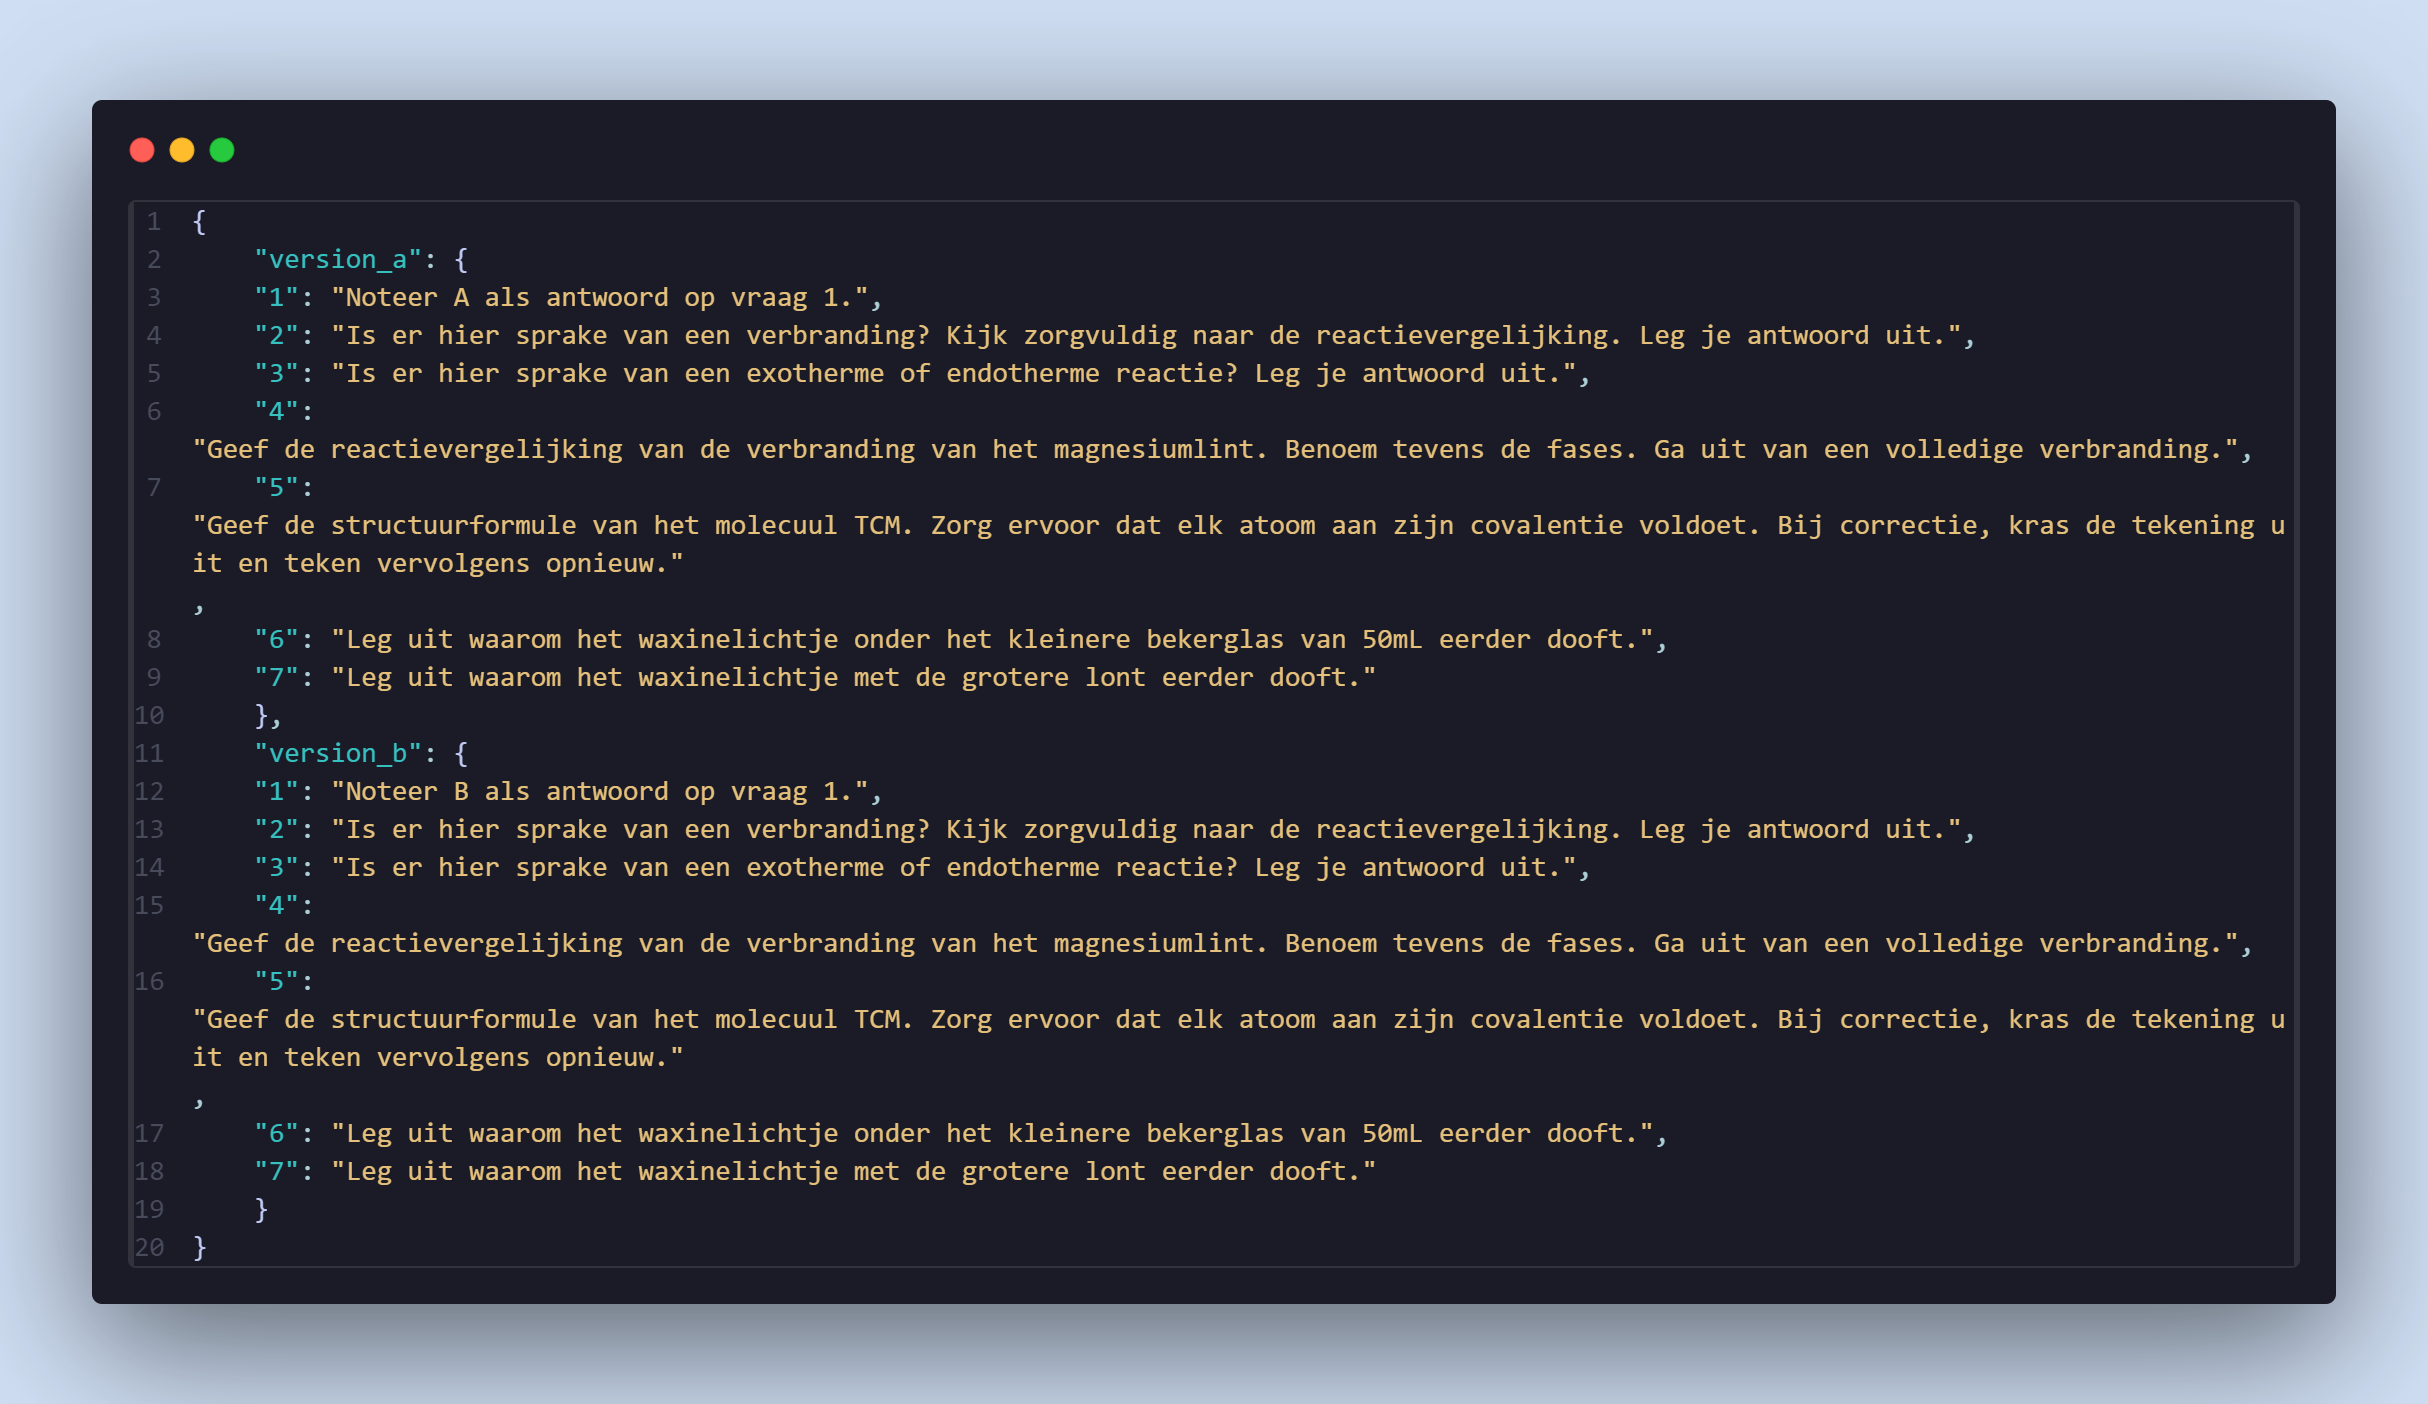
\includegraphics[width=0.6\textwidth]{./images/methoden/nakijken/json_structuur.png}
    \caption{JSON formaat}
    \label{fig:json_formaat}
\end{figure}
Je ziet hier ook versies staan. Later in het programma wordt daartussen onderscheid gemaakt. Er is voor een JSON-formaat gekozen, omdat je zo snel en gemakkelijk de vragen, rubrics en context in kan voeren. Het ophalen van die data is dan ook weer gemakkelijk met Python-code, zoals hieronder wordt getoond. Deze JSON-bestanden worden opgehaald met bijvoorbeeld de functie \ref{fig:vragen_inladen}.\\
\begin{figure}[H] % Position 'h' means 'here'
    \centering
    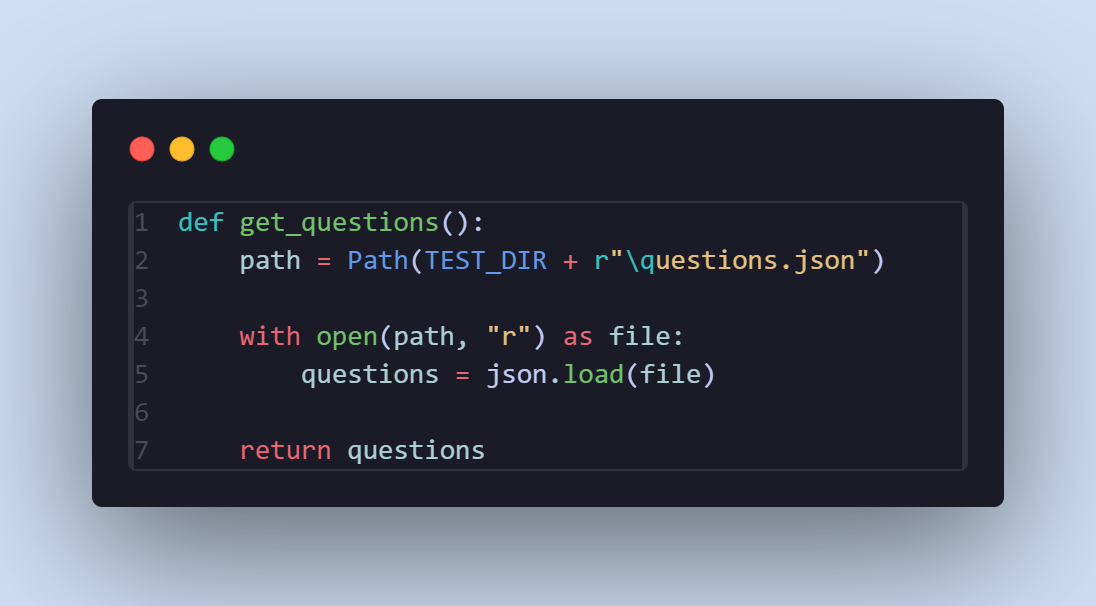
\includegraphics[width=0.8\textwidth]{./images/methoden/nakijken/load_questions.png}
    \caption{In laden van vragen}
    \label{fig:vragen_inladen}
\end{figure}
Hierdoor heeft ons programma toegang tot de context van de vraag, de rubric van de vraag en de vraag zelf. 
\\\\
\textbf{Het inladen van de studenten antwoorden:}
Van de inscanner krijg je een heel groot JSON-bestand terug. Het is erg lastig om hier meer te werken, omdat alle base64 encoded data van elke vraag erin staat. Deze data is louter voor vraag 5 nodig. De volgende code lost dat op \ref{fig:json_transformn}.

\begin{figure}[H] % Position 'h' means 'here'
    \centering
    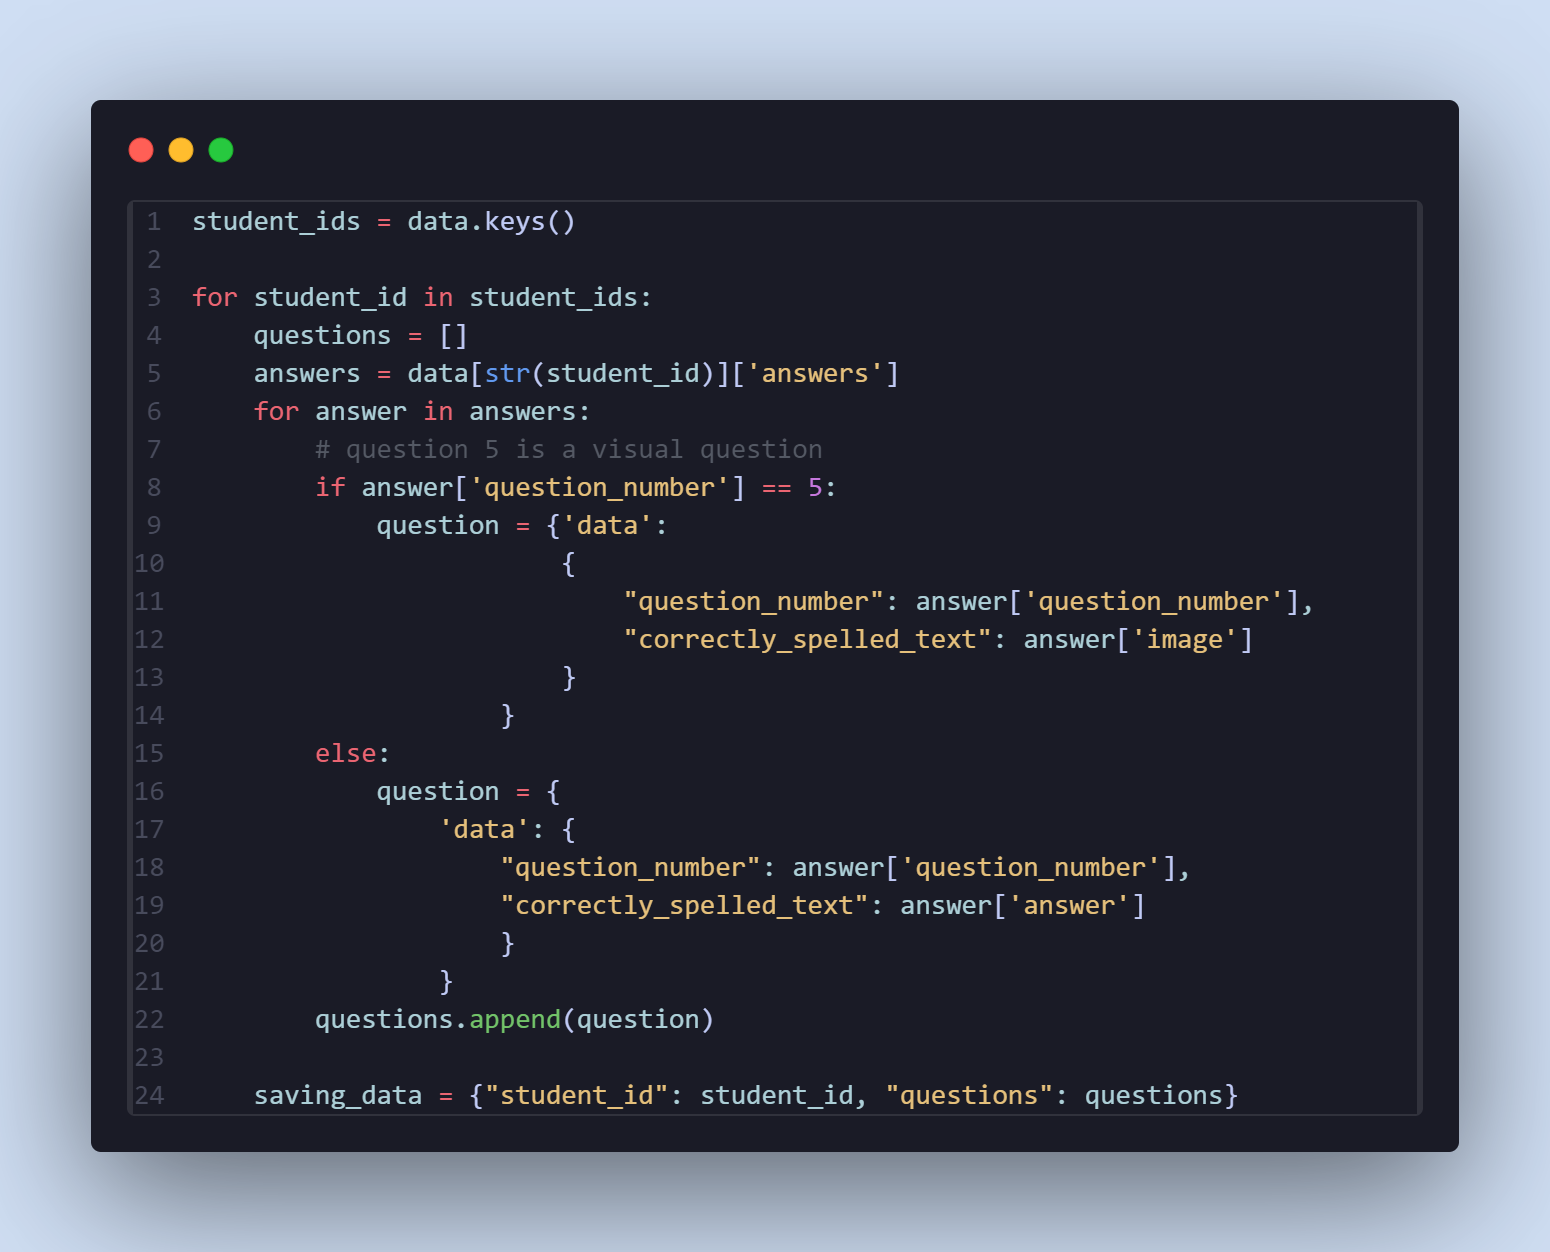
\includegraphics[width=0.8 \textwidth]{./images/methoden/nakijken/change_json.png}
    \caption{JSON omzetten}
    \label{fig:json_transformn}
\end{figure}
Hierna worden ze in individuele JSON-bestanden gezet waarna ze in het programma worden ingescand met de volgende functie \ref{fig:add_student}.
\begin{figure}[H] % Position 'h' means 'here'
    \centering
    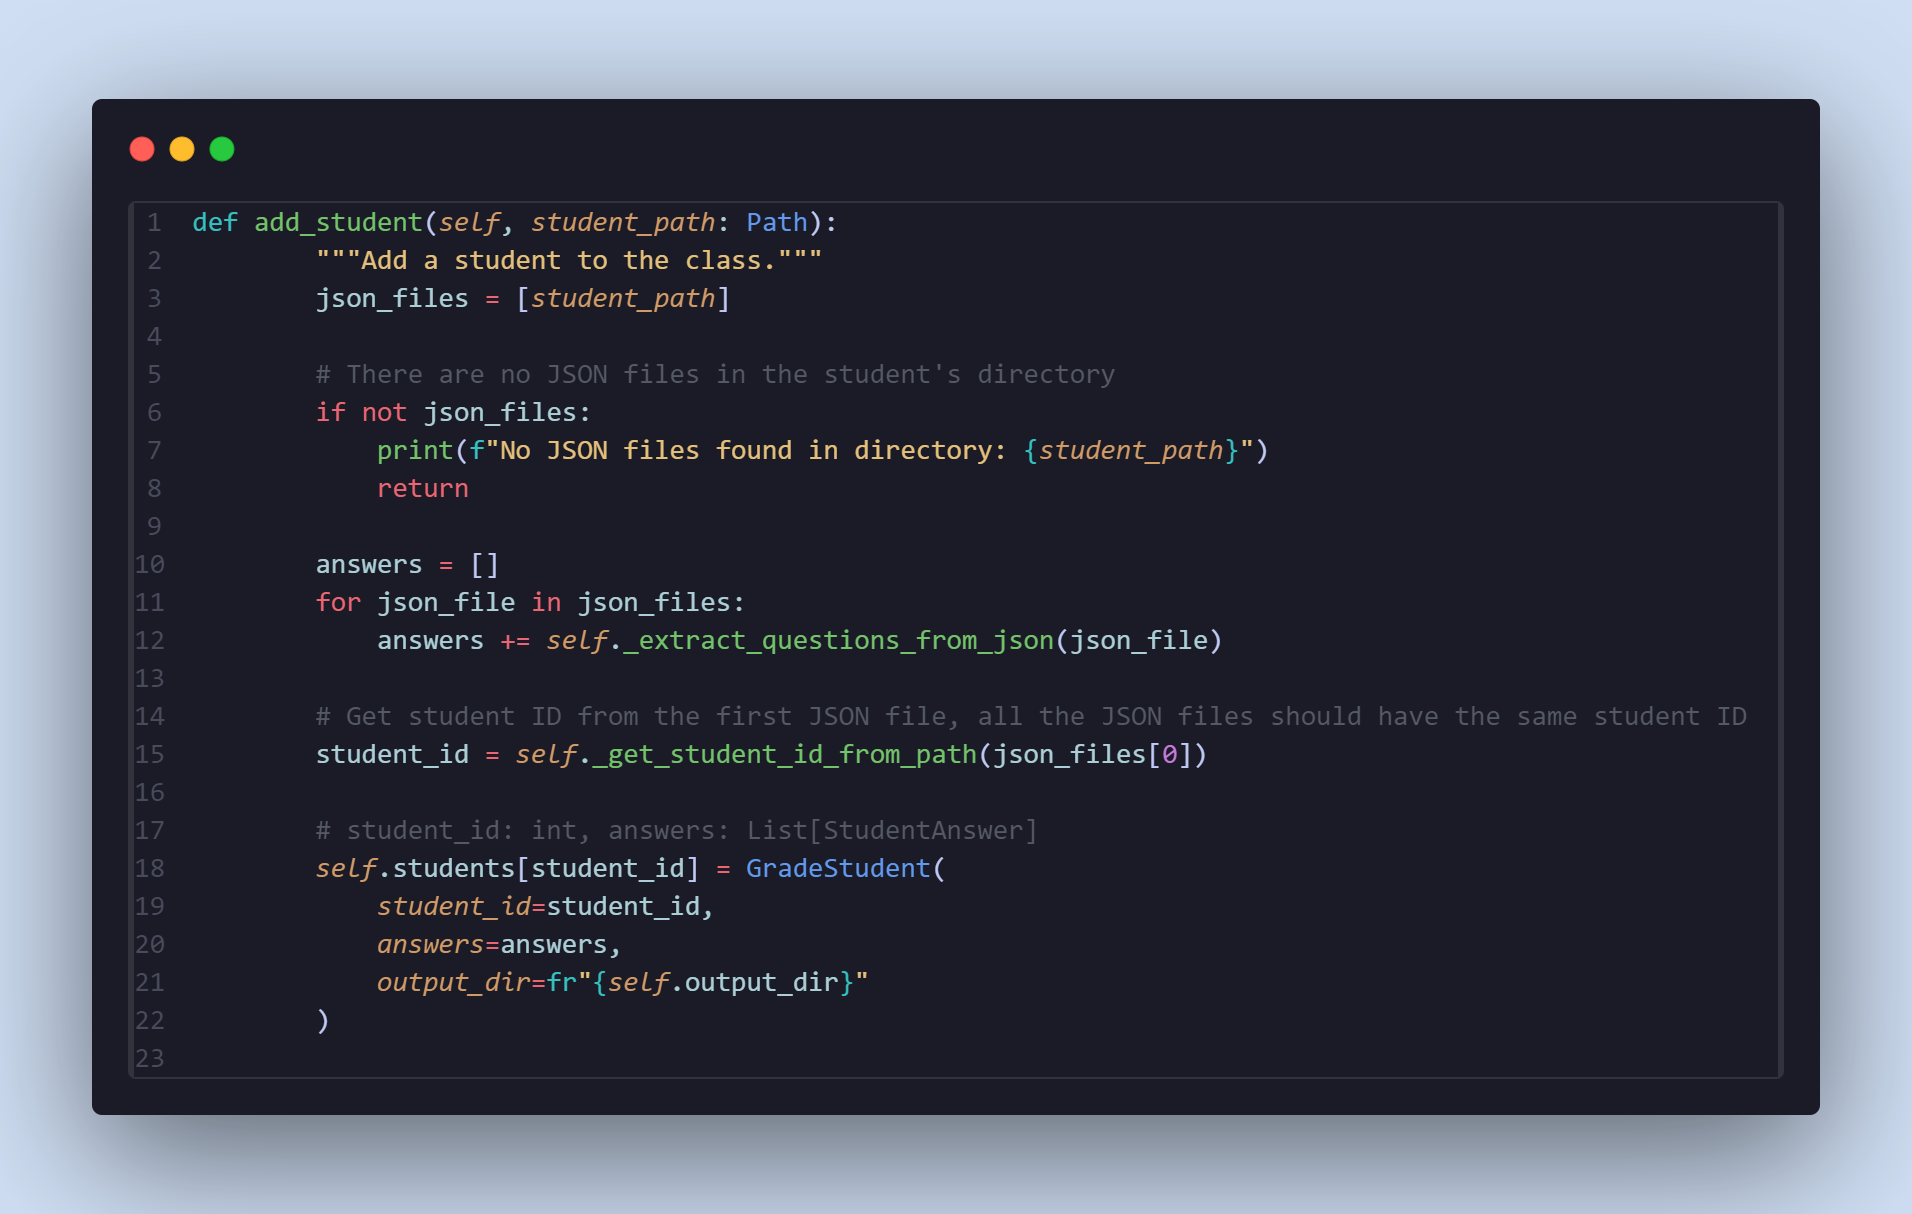
\includegraphics[width=0.9 \textwidth]{./images/methoden/nakijken/add_student.png}
    \caption{Student toevoegen}
    \label{fig:add_student}
\end{figure}
Nu is de student toegevoegd aan de klas en kan ons programma bij deze zijn antwoorden. Dit doen we in een for-loop waarbij we itereren over het mapje met alle JSON-bestanden van studenten.
\\ \\
\textbf{Het nakijken per vraag:} \\
Om een vraag na te kijken maken wij een request naar of de OpenAI-api of de Gemini-API. Deze request sturen wij met de volgende codes \ref{fig:OpenAI_request} \ref{fig:gemini_reques}.

\begin{figure}[H] % Position 'h' means 'here'
    \centering
    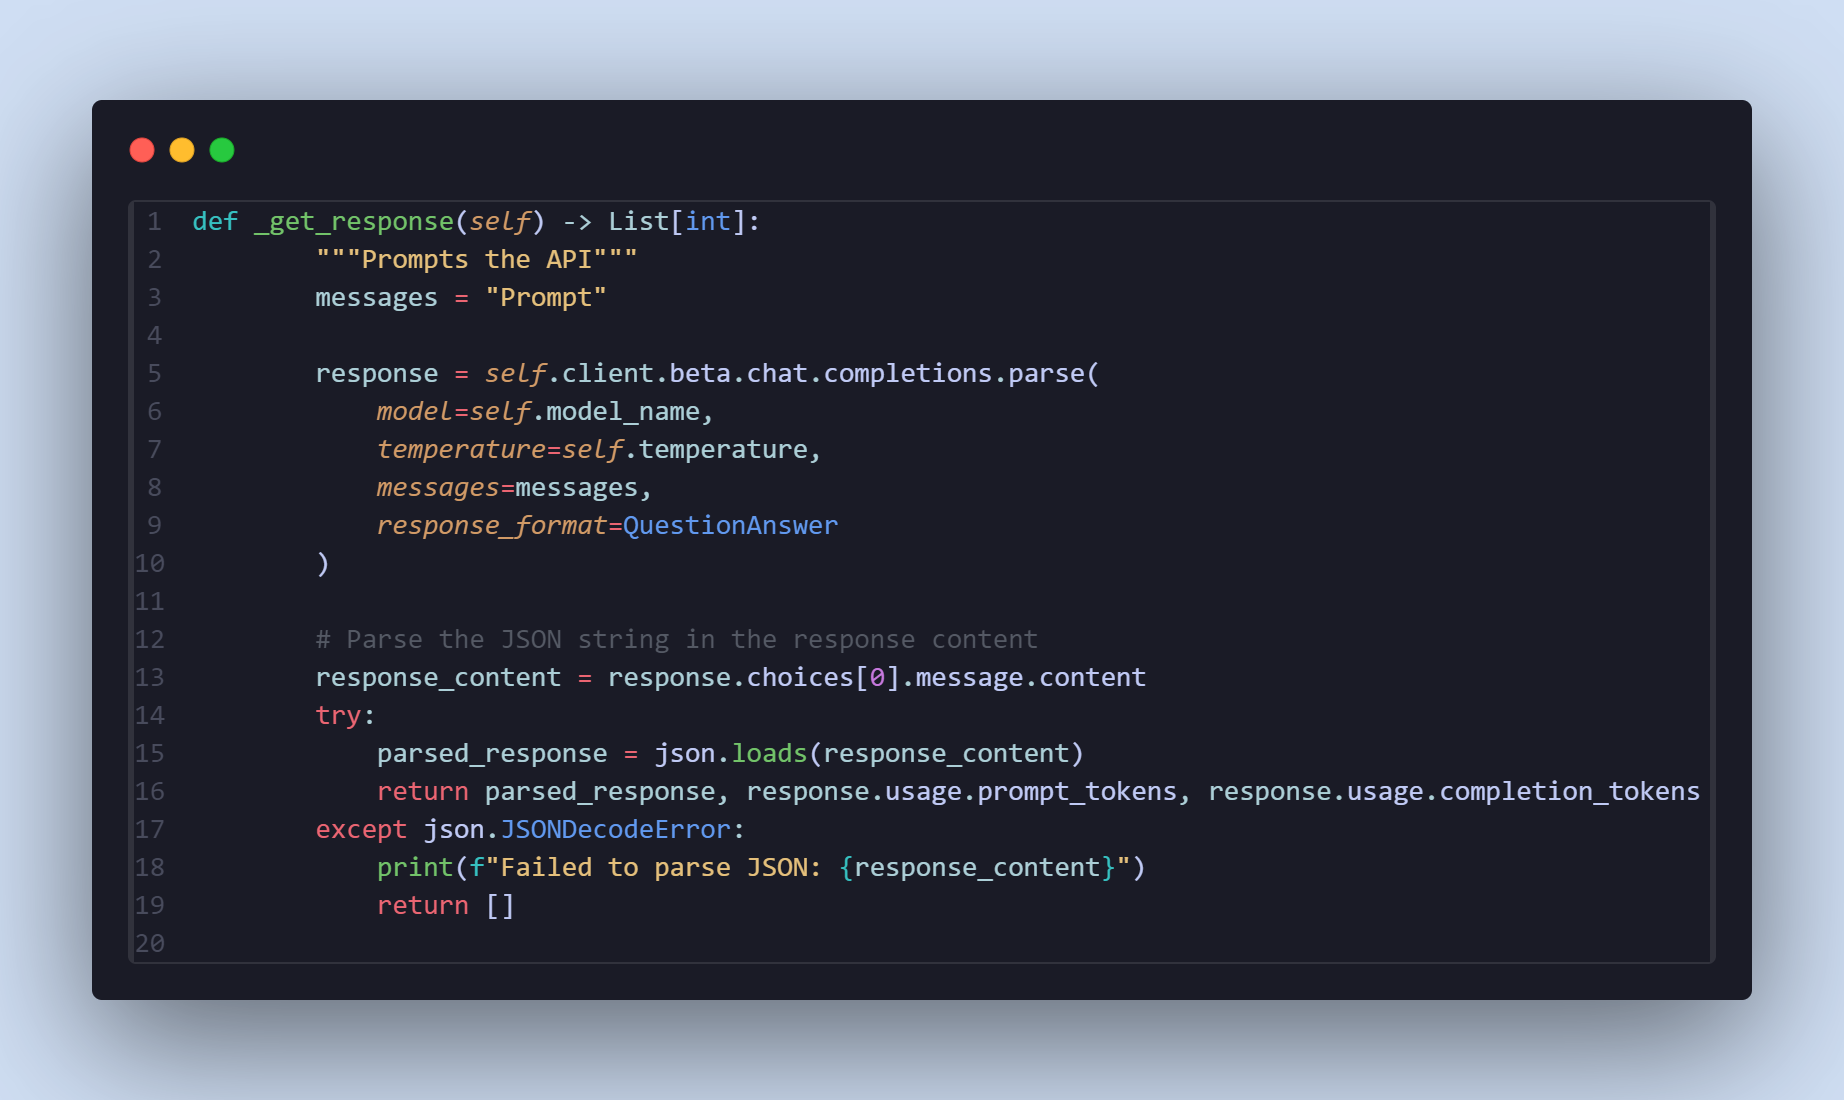
\includegraphics[width=0.9 \textwidth]{./images/methoden/nakijken/get_response.png}
    \caption{Request OpenAI}
    \label{fig:OpenAI_request}
\end{figure}
\begin{figure}[H] % Position 'h' means 'here'
    \centering
    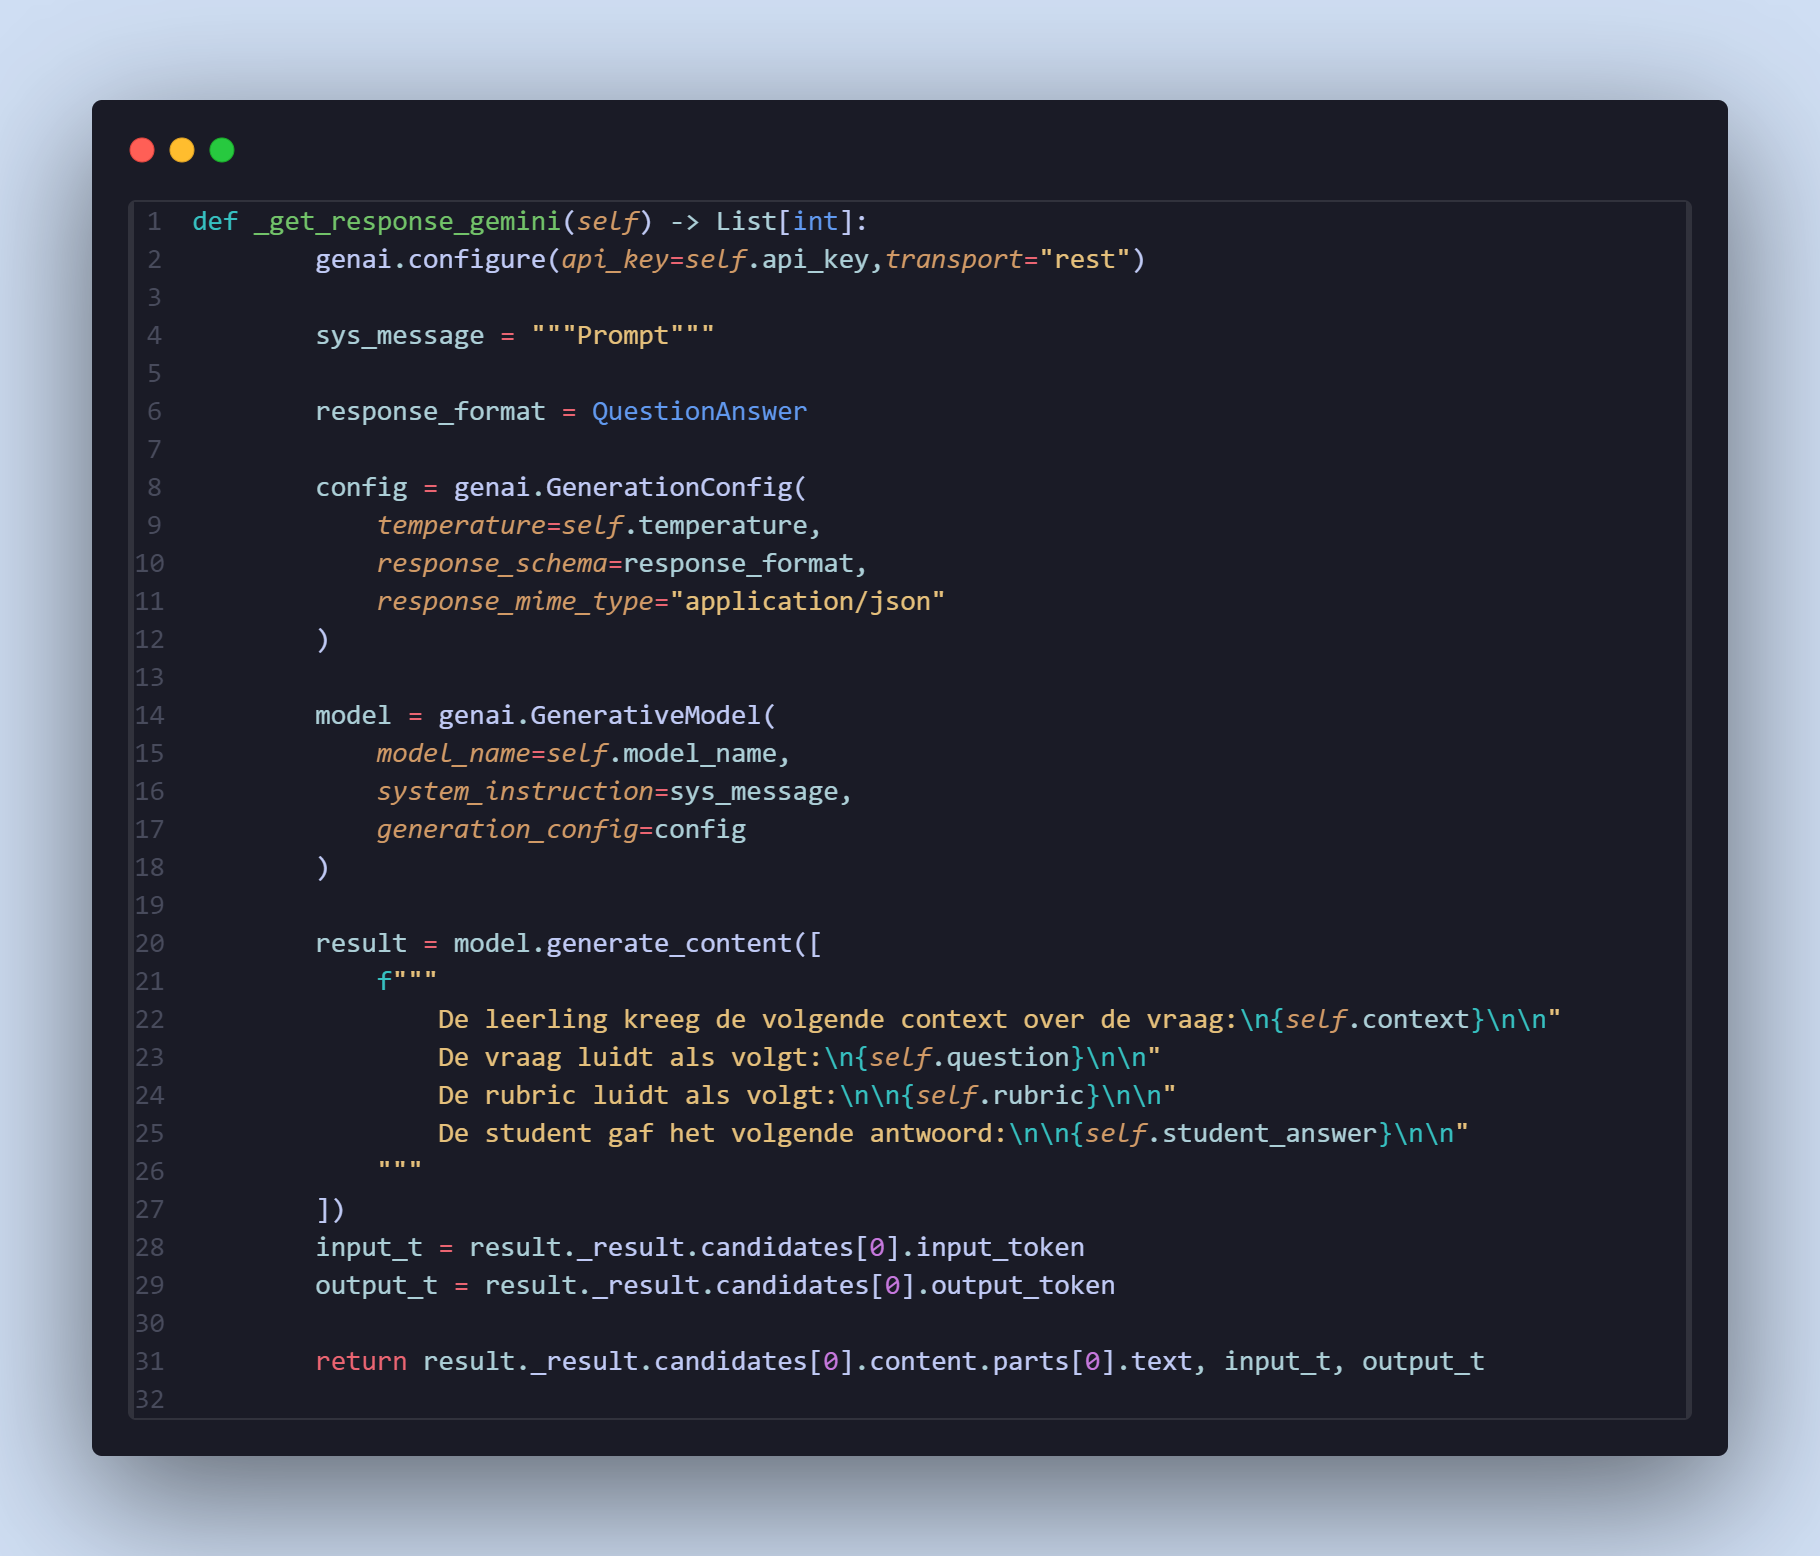
\includegraphics[width=0.9 \textwidth]{./images/methoden/nakijken/response_gemini.png}
    \caption{Request Gemini}
    \label{fig:gemini_reques}
\end{figure}
We sturen per vraag een aantal dezelfde requests om hallucinaties te voorkomen. Dit idee komt uit het volgende artikel uit het tijdschrift Nature (\cite{Farquhar2024}). Deze requests sturen we asynchroon op de volgende manier \ref{fig:async}.
\begin{figure}[H] % Position 'h' means 'here'
    \centering
    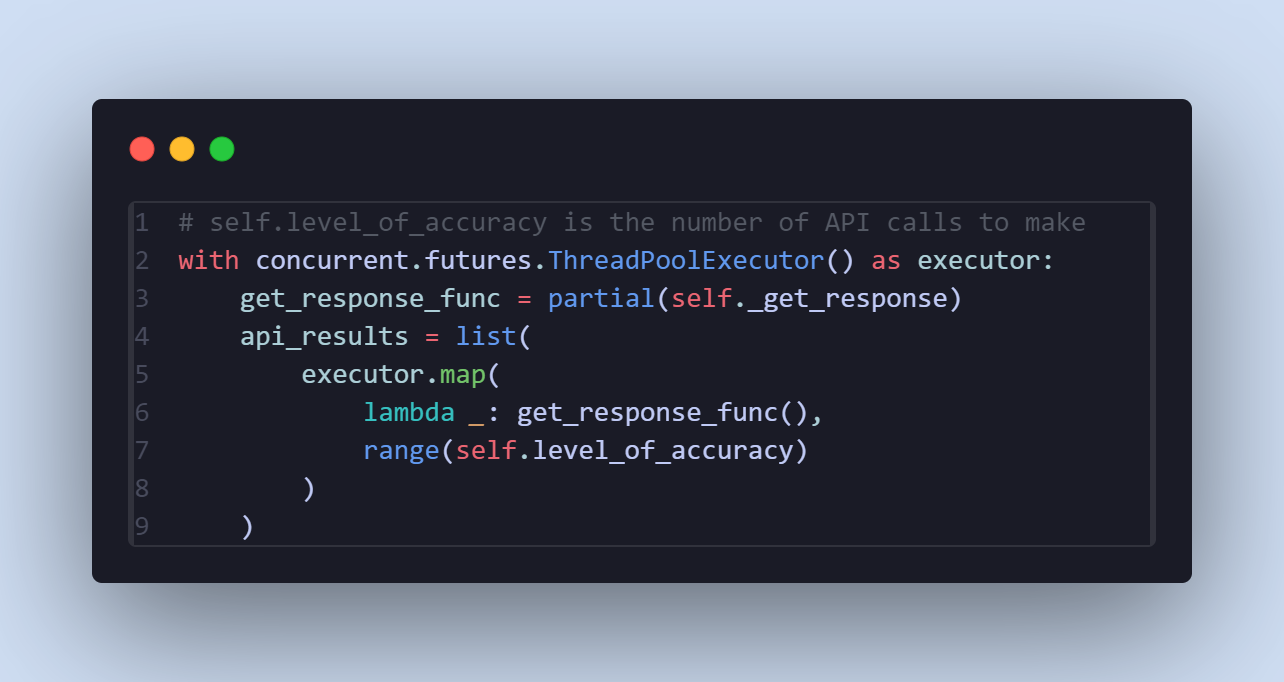
\includegraphics[width=0.9 \textwidth]{./images/methoden/nakijken/threading.png}
    \caption{Asynchrone requests}
    \label{fig:async}
\end{figure}

Als laatste tellen we van elke request op hoe vaak een rubricpunt wel of niet gegeven wordt. Het meest voorkomende antwoord veronderstellen wij als de waarheid. Deze slaan we dan ook op. Het optellen kan simpelweg gedaan worden met een for-loop waarbij je itereert over de resultaten.\vspace{0.25cm}
\\

\textbf{Het nakijken per student:} \\
Alle resultaten per student zijn al ingeladen volgens hierboven beschreven methode. Het nakijken, het managen van een student en het managen van een klas zijn allemaal gescheiden klassen volgens OOP. Om een student na te kijken hoef je dan alleen maar de volgende functie asynchroon voor alle gemaakte vragen van een student aan te roepen \ref{fig:Vraag_nakijken}. 

\begin{figure}[H] % Position 'h' means 'here'
    \centering
    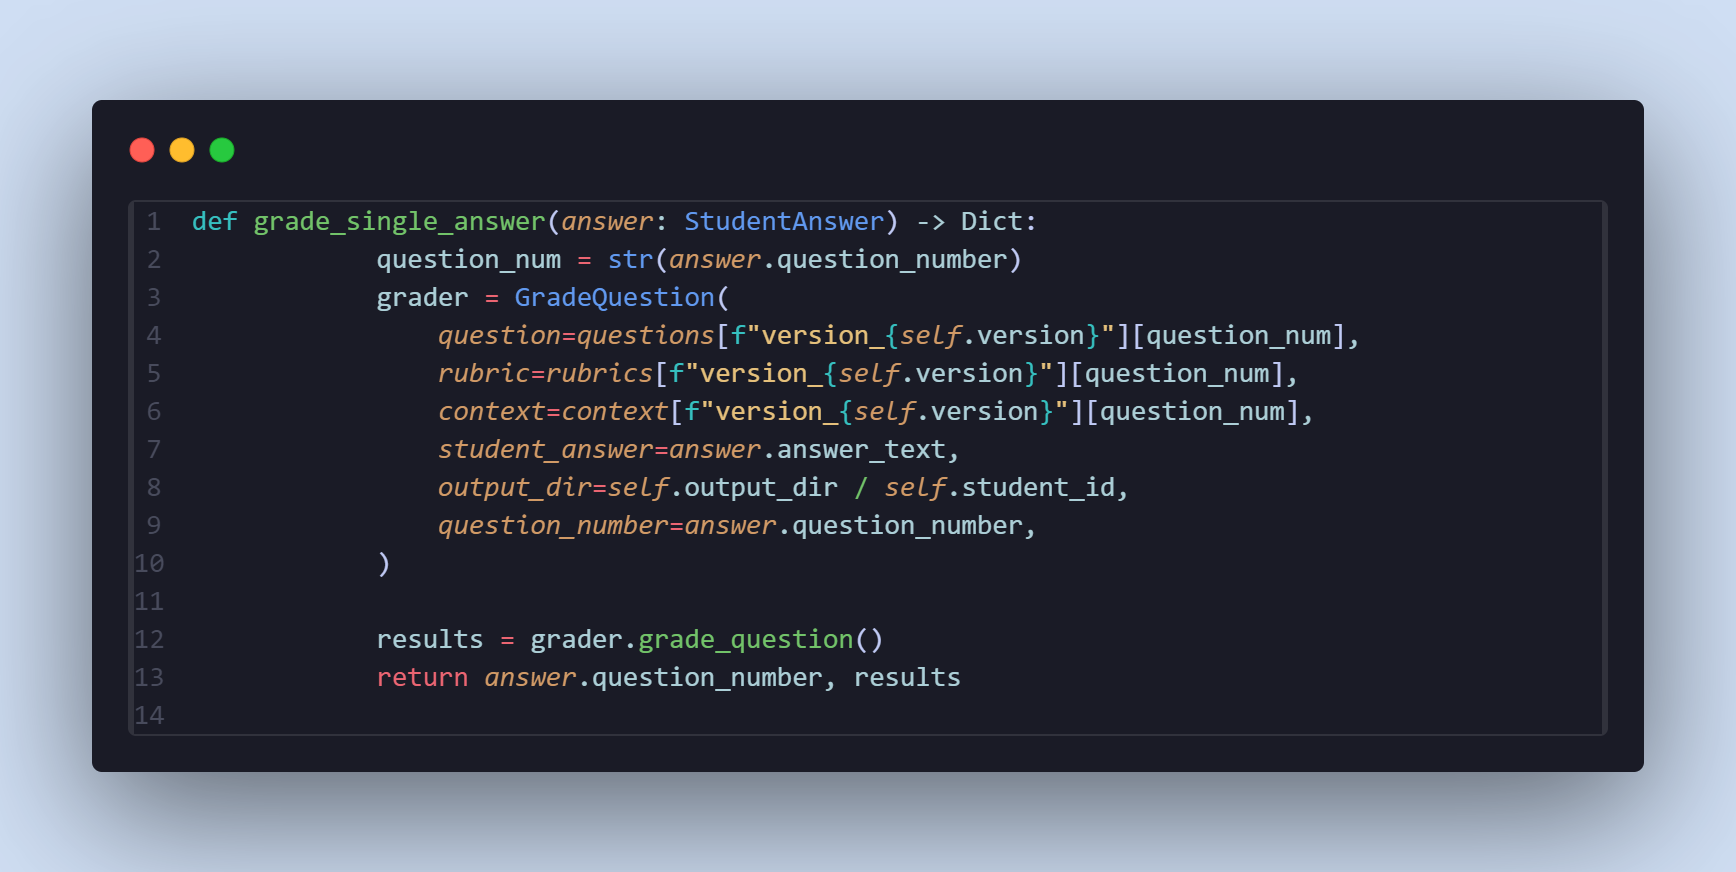
\includegraphics[width=0.8 \textwidth]{./images/methoden/nakijken/grade_question.png}
    \caption{Vraag nakijken}
    \label{fig:Vraag_nakijken}
\end{figure}
Deze resultaten worden dan opgeslagen. En dan is één student nagekeken.
\\ \\
\textbf{Het nakijken van een klas:}\\
Om de klas na te kijken maken we dus steeds een student-object. Als we de klas willen nakijken, dan itereren we over alle student-objecten en gebruiken we de functie om hem na te kijken. Met 10 requests per vraag, 7 vragen, 30 studenten en standaard rate-limits doet hij er iets meer dan 3 minuten over.
\\ \\
\textbf{Het optimaliseren van modelparameter}
Om het AI-model zo goed mogelijk te laten presteren bij het nakijken van scheikunde toetsen, moeten de parameters van het model zorgvuldig worden afgestemd. Twee belangrijke parameters die hierbij een grote rol spelen zijn de temperatuur en de promptformulering.

\begin{itemize} 
\item \textbf{Temperatuur:}
De temperatuur beïnvloedt de "creativiteit" van de gegenereerde antwoorden. Bij een lage temperatuur (bijvoorbeeld 0.2) worden antwoorden consistenter en voorspelbaarder, wat belangrijk is bij het nakijken van open vragen met objectief juiste antwoorden. Bij hogere temperaturen kunnen antwoorden diverser, maar minder betrouwbaar worden. Daarom voeren we meerdere experimenten uit om de optimale temperatuur te vinden (\cite{peeperkorn2024temperature}).
\item \textbf{Promptformulering:}  
De prompt bepaalt hoe duidelijk de vraag, rubric, context en opdracht van het nakijken aan het model wordt gepresenteerd. Een goed geformuleerde prompt helpt het model om de vraag en verwachtingen correct te interpreteren (\cite{qian2024long}). We testen verschillende versies van prompts, zoals:  
    \begin{itemize}  
        \item Een korte set instructies (Bij te veel instructies raakt het model misschien verward)
        \item Een lange set instructies (Meer instructies geeft wellicht een duidelijker beeld van de opdracht) 
    \end{itemize}
\end{itemize}

\noindent De combinatie van een optimale temperatuur en een zorgvuldig opgebouwde prompt zorgt ervoor dat de feedback nauwkeuriger en betrouwbaarder wordt. Dit wordt getest door verschillende instellingen uit te proberen op een set van voorbeeldantwoorden en de uitkomsten te vergelijken met menselijke beoordelingen. Per vraag testten we drie verschillende antwoorden. Een goed antwoord, en helemaal fout antwoord en een half goed, half fout antwoord.


\pagebreak



\subsubsection{Analyseren}
\begin{tabularx}{\linewidth}{@{}ll}
    \textbf{Eigenaar: } & \textit{Joost} \\
    \textbf{Doel(en): } & 
        \makecell[tl]{
            $\bullet$ Docenten inzicht geven in de resultaten van een klas en zien welke \\onderwerpen aandacht nodig hebben.\\
            $\bullet$ Docenten inzicht geven in de betrouwbaarheid van de toets, door opvallende \\ statistische resultaten weer te geven.\\
        } \\
    \textbf{Subvragen: } & 
        \makecell[tl]{
            $\bullet$ Hoe doe een een statistische analysen van toetsresultaten? \\
            $\bullet$ Hoe geef je deze resultaten overzichtelijk weer? \\
        }\\
    \textbf{Kader(s): } & 
        \makecell[tl]{
            $\bullet$ Statistiek \\
            $\bullet$ UI (user interface) \\
        }\\
    \parbox[t]{3cm}{\raggedright \textbf{Geschatte  tijdskosten:} } & 15 uur \\
\end{tabularx}
\\
\begin{multicols}{2}
    
Bij het inscannen gaan we onderzoek doen naar welke statistische berekeningen nodig zijn voor correct analyse. Ook gaan we uitzoeken wat voor interface nodig is en welke berekeningen of dingen we aan een docent kunnen laten zien om een duidlijk beeld te krijgen van de staat van de klas. We gaan gebruik maken van internet. \\
\\
Ook gaan we een test website maken met VueJs (\cite{vuejsManual}). De code voor deze website is open-source en is te vinden op \url{https://github.com/Thannie/Test-Analyzer}.
Daarnaast hosten we zelf de website op \url{https://toetspws.web.app/analyze}, waar nu een testversie van een analyseer app staat met test data. In het analyseer menu in de fold-out correlaties is een mooie correlatie matrix te zien en in het grafiek menu een interactieve normaalverdeling als op bereken wordt geklikt. De interface hebben we gemaakt met Vuetify (\cite{vuetifyManual}), dat zorgt voor de mooie menu's  (merk op dat \url{https://toetspws.web.app/scan} naar de inscan website gaat, die gebruikt maakt van onze inscan API).\\
\\
\end{multicols}

\pagebreak

\subsubsection{Enquete}
\begin{tabularx}{\linewidth}{ll}
    \textbf{Eigenaar: } & \textit{Jonathan en Joost} \\
    \textbf{Doel(en): } & 
        \makecell[tl]{
            $\bullet$ Inzicht krijgen in de mogelijkheid in de integratie van AI \\ bij docenten op Het Amsterdams Lyceum \\
        } \\
    \textbf{Subvragen: } & 
        \makecell[tl]{
            $\bullet$ Hoe neem je een betrouwbare enquête? \\
            $\bullet$ Hoe zorg je ervoor dat mensen jouw enquête willen invullen? \\
        }\\
    \textbf{Kader(s): } & 
        \makecell[tl]{
            $\bullet$ Enquete maken\\
            $\bullet$ Overtuigende mail\\
        }\\
    \parbox[t]{3cm}{\raggedright\textbf{Geschatte  tijdskosten:} } & 20 uur \\
\end{tabularx}
\begin{multicols}{2}
Om te testen of docenten überhaupt open staan voor een ai model hebben we een enquête verstuurd naar alle docenten van Het Amsterdams Lyceum. 
Om een betrouwbare enquête te maken moet je als eerste het doel van de enquête duidelijk hebben. In ons onderzoek waren dat de volgende:
\begin{minipage}{\linewidth}
\begin{itemize}
    \item target voor ons programma stellen
    \item mogelijke acceptatie in kaart brengen
\end{itemize}
\end{minipage}
Daarnaast moet elke vraag ook een duidelijk doel hebben, anders is het mogelijk dat je 2x dezelfde vraag stelt of naar informatie gaat vragen niet niet relevant is.\\
Ten slotte moesten we bij elke vraag nagaan of de vraag op verschillende manieren geïnterpreteerd kan worden.\\
\end{multicols}%

\pagebreak
\begin{longtable}{p{0.5\linewidth}|p{0.25\linewidth}|p{0.25\linewidth}}
    Vraag & Doel & Verklaring \\
    \endhead
    \hline 
    \begin{minipage}[t]{\linewidth}
        \textbf{1. Wat is uw vakgebied? (Indien meerdere, kies vak met meeste uren a.u.b.) }
        \hspace{4em} Vakken        
    \end{minipage} & kunnen filtreren op vakgebied en vakgroep ($\alpha, \beta, \gamma$) & \\
    \hline 
    \begin{minipage}[t]{\linewidth}
        \textbf{2. Hoeveel jaar bent u al docent? }
        \begin{itemize}
            \item 1-5 jaar
            \item 5-10 jaar
            \item Meer dan tien jaar
            \item Minder dan één jaar
        \end{itemize}
    \end{minipage} & kunnen filtreren op lesgeef ervaring & \\
    \hline 
    \begin{minipage}[t]{\linewidth}
        \textbf{3. Bent u bekend met het concept van ( generatieve ) AI? }
        \begin{itemize}
            \item Ja, ik ben goed op de hoogte
            \item Ja, ik heb er wel eens over gehoord
            \item Nee, ik ben niet bekend met deze technologie
        \end{itemize}
    \end{minipage} & kunnen filtreren op ai ervaring & \\
    \hline 
    \begin{minipage}[t]{\linewidth}
        \textbf{4. Wat zouden voor u redenen zijn om AI te gebruiken voor het nakijken van proefwerken? (Meerdere antwoorden mogelijk) }
        \begin{itemize}
            \item Tijdbesparing
            \item Objectiviteit in de beoordeling
            \item Vermindering van de werkdruk
            \item Snelheid van de terugkoppeling naar studenten
            \item Betere nauwkeurigheid
            \item Ik zou nooit overwegen AI hierbij te gebruiken
            \item Anders: \textit{zelf invullen}

        \end{itemize}
    \end{minipage} & weten wat het hoofddoel moet zijn van ons programma en wat waar we minder aandacht aan kunnen besteden & optie 1 en 3 lijken op elkaar, maar zijn niet hetzelfde dat is later ook deels terug te zien in de resultaten\\
    \hline 
    \begin{minipage}[t]{\linewidth}
        \textbf{5. Wat zijn uw belangrijkste zorgen bij het gebruik van AI voor het nakijken van proefwerken? }
        \begin{itemize}
            \item Gebrek aan menselijke empathie in de beoordeling
            \item Mogelijke technische fouten
            \item Onvoldoende aandacht voor subjectieve antwoorden
            \item Data- en privacykwesties van studenten
            \item Oneerlijke of bevooroordeelde beoordelingen
            \item Afhankelijkheid van technologie
            \item Anders: \textit{zelf invullen}
        \end{itemize}
    \end{minipage} & weten waar we op moeten focussen en wrten of bepaalde problemen een grote bottleneck zullen zijn voor de acceptatie van ons programma voor docenten & \\
    \hline 
    \begin{minipage}[t]{\linewidth}
        \textbf{6. Denkt u dat AI zelfstandig toetsen zou kunnen nakijken}
        \begin{itemize}
            \item Ja
            \item Nee
            \item Weet ik niet
        \end{itemize}
    \end{minipage} & weten hoe positief docenten in een mogelijkheid zijn en om te vergelijken met vakgebied en lesgeef ervaring & \\
    \hline 
    \begin{minipage}[t]{\linewidth}
        \textbf{7. Hoeveel leerlingen trekken uw beoordeling per toets \- terecht of niet \- in twijfel? (Een getal)}\\
        \vspace{4em} Zelf een getal invullen
        \end{minipage} & 
        \begin{minipage}[t]{\linewidth}
            Een objectief target halen waarmee we ons programma kunnen vergelijken:\\ 
            meer oneens is slechter of te streng naar gekeken \\ 
            te weinig is te makkelijk nagekeken 
        \end{minipage}
        & \begin{minipage}[t]{\linewidth}
            Hier is een afweging gemaakt tussen een makkelijk te lezen vraag en een wiskundig correcte vraag. Het is hier niet expliciet gezegt dat het per toets per klas (van ongeveer 30 leerlingen) is.
        \end{minipage}\\
    \hline 
    \begin{minipage}[t]{\linewidth}
        \textbf{8. Welke invloed denkt u dat de inzet van AI kan hebben op de relatie tussen docent en student? (Open vraag) }\\
        \vspace{4em} Zelf een getal invullen

    \end{minipage} & Als docenten nog wat kwijt willen kunnen ze dat hier doen, misschien staat er wat interessants tussen & \\
\end{longtable}

\pagebreak

\begin{multicols}{2}
Ons 2e doel van dit onderdeel was: \textbf{Hoe zorg je ervoor dat mensen jouw enquête willen invullen?}\\
Uit ons kleine omgevingsonderzoek blijkt dat docenten van Het Amsterdams Lyceum niet vaak reageren op (onbelangrijke) mail. Een score van 30\% zou al aan de hoge kant zijn. We hebben een zakelijk mail proberen samen te stellen die ervoor zorgt dat docenten wilden reageren. \\
\fbox{\begin{minipage}{\linewidth}
    
Geachte docenten van Het Amsterdams Lyceum,\\
\\
In het kader van ons profielwerkstuk, maken wij een programma dat dat toetsen kan inscannen, nakijken en analyseren. \\
Daarnaast zijn we geïnteresseerd in hoe docenten denken over het nakijken met AI, hierbij zouden wij graag uw hulp willen.\\
\\
https://forms.office.com/e/j5cYFrAy7p 
\\
Hoogachtend,\\
\\
Joost Koch \& Jonathan Wijker
\end{minipage}}
Op dit mail hebben we 22 reacties gekregen. Dat vonden wij redelijk tegenvallen.
Een reden voor deze teleurstellende respons zou kunnen zijn dat we de mail verstuurd hebben op donderdag 17 oktober. Dat was de donderdag voor de activiteitenweek, waardoor docenten met uitzicht op een vakantie misschien geen zin hadden in het invullen van een PWS-enquête.\\
\\
Daarna hebben de gekeken wat het ideale moment zou zijn voor een docent om zin te hebben in het invullen van een enquête. Toen kwamen we na overleg met diverse docenten erachter dat de week voor de toetsweek het rustigst is, want de meeste docenten hebben alle lesstof al behandeld, geen toetsen om na te kijken en hebben de toetsen en SE's al af en ingelevert.  \\
\\
We hebben ons tweede mail op de maandag voor de toetsweek gestuurd. We hebben ook de docenten extra proberen te vleien door duidelijk aan te geven dat het weinig tijd kost en dat we weten hoe druk docenten het eigenlijk hebben.
\fbox{\begin{minipage}{\linewidth}
    
Geachte docent,\\
\\
Onlangs hebben wij u een enquête gestuurd en we hebben al wat reacties mogen ontvangen, bedankt daarvoor.\\
We snappen dat u het komende tijd druk heeft met de toetsweek, maar hopen dat u komende week ergens een gaatje van 2-3 minuten kunt vinden om alsnog onze enquête in te vullen. Dit zouden we erg waarderen!\\
 \\
https://forms.office.com/e/j5cYFrAy7p\\
\\
Hoogachtend,\\
 \\
Joost Koch \& Jonathan Wijker
\end{minipage}}
Dit leverde 28 extra responses op, waardoor we op een totaal van 50 zitten. Wij waren heel tevreden met deze hoge response. \\

We moeten er wel rekening mee houden dat sommige secties misschien minder zullen hebben gereageerd, waardoor ons resultaat over die sectie minder betrouwbaar zal zijn.\\
\\
Voor het analyseren gaan we Google Sheet pivot tables gebruiken om snel verbanden tussen de data te zien. Ook zullen we kijken of ChatGPT of Google Gemini relevante ontdekkingen kunnen doen in de data. 


\end{multicols}
\pagebreak

\subsubsection{Praktijktest}
\begin{tabularx}{0.5\linewidth}{ll}
    \textbf{Eigenaar: } & \textit{Jonathan} \\
    \textbf{Doel(en): } & 
        \makecell[tl]{
            $\bullet$ Een toets maken die duidelijk is voor 3e klassers\\
            $\bullet$ Een toets nakijken met onze programmas\\
        } \\
    \textbf{Subvragen: } & 
        \makecell[tl]{
            $\bullet$ Hoe maken we een toets die duidelijk is voor 3e klassers? \\
            $\bullet$ Hoe kijken we een toets na met onze programmas? \\
        }\\
    \textbf{Kader(s): } & 
        \makecell[tl]{
            $\bullet$ Toetsen maken / scheikunde \\
            $\bullet$ Programma testen \\
        }\\
    \parbox[t]{3cm}{\raggedright\textbf{Geschatte  tijdskosten:} } & 15 uur \\
\end{tabularx}

\subsubsection*{Onderzoekspopulatie}
De deelnemers aan dit onderzoek zijn leerlingen uit \emph{3 VWO} die een scheikundetoets afleggen als onderdeel van hun reguliere curriculum. De selectie van de klas gebeurt in overleg met de betrokken docent, waarbij gestreefd wordt naar een representatieve afspiegeling van het niveau en de voorkennis van de leerlingen. Het verwachte aantal deelnemers ligt tussen de 20 en 30 leerlingen, zodat er voldoende data verzameld kan worden voor de analyse.

\subsubsection*{Materiaal}
\paragraph{De toets} 
De scheikundetoets bestaat uit een set open vragen en één tekenvraag ontwikkeld door een vakdocent en ons. Deze vraag gaat over het tekenen van chloroform. De toets behandelt leerstof uit het voorafgaande hoofdstuk of thema.
\begin{itemize}
    \item \textbf{Open vragen:} 6 vragen die inzicht vereisen in probleemoplossend denken, redeneren en toepassen van concepten.
    \item \textbf{Tekenvraag:} één vraag dat het grafische vermogen van het model test.
\end{itemize}

\paragraph{AI Correctiemodule} 
Er wordt gebruikgemaakt van een prototype (computer)programma. Dit programma maakt gebruik van een Large Language Model (LLM). Elke toets zal door meerdere modellen worden nagekeken. Dit is verder uitgewerkt in (\ref{methode-nakijken}), waarin de methode voor de nakijkmodule nader wordt beschreven.
\begin{itemize}
    \item \textbf{Antwoordmodellen (rubrics)} voor de open vragen, ontwikkeld in samenspraak met een vakdocent.
    \item \textbf{De modellen} om de vragen na te kijken.
\end{itemize}

\paragraph{Analyse-instrumenten} 
Naast de AI-module wordt een statistisch softwarepakket gebruikt voor het verwerken van de resultaten en het genereren van overzichten (gemiddeldes, spreidingen, item-analyse). Deze worden niet in de resultaten van de toets, maar in de resultaten van het nakijken verwerkt, omdat het daar meer mee te maken heeft.

\subsubsection*{Procedure}

\paragraph{Toetsafname} 
De toets wordt gedurende een reguliere lestijd afgenomen in de klas, onder toezicht van de docent en onszelf. Alle leerlingen maken dezelfde toets zonder toegang tot internet of ongeoorloofde hulpmiddelen. De verwachting is dat de afname ongeveer 30 minuten duurt.

\paragraph{Verzamelen van Antwoorden} 
Na afloop van de toets leveren de leerlingen hun antwoorden in. De antwoorden worden gedigitaliseerd met behulp van het inscan programma. Mogelijke foutieve beoordelingen zullen hier dus ook vanaf hangen.

\paragraph{Automatische Correctie} 
De ingevoerde leerlingantwoorden worden vervolgens door het AI-systeem verwerkt. Dit is verder uitgewerkt in (\ref{methode-nakijken}), waarin de methode voor de nakijkmodule nader wordt beschreven.


\paragraph{Validatie door Mens} 
Vervolgens kijkt een mens de toets handmatig na. Deze menselijke beoordeling wordt als de gouden standaard beschouwd, waarmee de AI-resultaten worden vergeleken.

\subsubsection*{Data-analyse}
Na het verzamelen van alle scores wordt de data geanalyseerd om:
\begin{itemize}
    \item De overeenstemming tussen de AI-scores en de menselijke (docent)scores te meten, bijvoorbeeld middels een correlatiecoëfficiënt of Cohen’s kappa.
\end{itemize}
Dit zal allemaal verwerkt worden in de resultaten van het nakijken.

\subsubsection*{Ethiek en Privacy}
Alle gegevens worden anoniem verwerkt en alleen gebruikt voor onderzoeksdoeleinden. De namen van leerlingen worden vervangen door leerlingennummers. De docent en leerlingen worden vooraf geïnformeerd over het doel van het onderzoek en geven toestemming voor hun deelname.




\pagebreak
\section{Resultaten}
\subsection{Inscannen}
\noindent Hieronder zijn een aantal tabellen te zien met de resultaten van het inscanonderdeel uitgelegd in de methode. \\
We hebben deze tabellen gekozen om te kijken wat de beste inputs voor ons inscansysteem zijn. \\
Een lagere score is beter dan een hogere score, want hoe meer fouten hoe hoger de score. Ook willen we liever een lage standaarddeviatie, want dan is ons model voorspelbaarder. \\
In de appendix is zijn een aantal test gegeven in een tabel met een quote van Johan Cruijff die een goed beeld geven van wat een score betekent en een aantal andere tests.\\
De resultaten zijn niet normaal verdeeld, omdat een score niet kleiner dan 0 kan zijn, daardoor zal die vaak hoger zijn dan je zou denken. Er wordt vooral gekeken naar verschillende standaarddeviaties ten opzichte van elkaar. 
\\
\noindent\href{https://docs.google.com/spreadsheets/d/1wbHiG81i-UJ18s6gP3i_WtsPD-FBQTqg7AwNjN8Rm2g}{Resultaten}

\noindent\begin{table}[H]
\caption{\# per model}
\label{fig:count-model}
\begin{tabularx}{\textwidth}{X *2{r}}
    \toprule
    \multicolumn{1}{c}{\textbf{Model}} & \multicolumn{1}{c}{\textbf{\#}} \\  % Changed
    \midrule
    gemini-1.5-flash-8b & 1125 \\
    gemini-1.5-pro-002 & 787 \\
    gemini-2.0-flash-exp & 1257 \\
    gpt-4o & 1029 \\
    gpt-4o-mini & 1167 \\
    \midrule
    \textbf{Totaal} & \textbf{5365} \\
    \bottomrule
    
\end{tabularx}%
\end{table}



\noindent\begin{table}[H]
\caption{score per model}
\label{fig:score-model}
\begin{tabularx}{\textwidth}{X *3{r}}
    \toprule
    \multicolumn{1}{c}{\textbf{Model}} & \multicolumn{1}{c}{\textbf{avg cor score}} & \multicolumn{1}{c}{\textbf{stdev cor score}} & \multicolumn{1}{c}{\textbf{avg cor change count}} \\
    \midrule
    gemini-1.5-pro-002 & 0.4838 & 0.4913 & 3.0851 \\
    gemini-2.0-flash-exp & 0.5874 & 0.5414 & 6.9880 \\
    gpt-4o-mini & 0.5905 & 1.6675 & 5.5089 \\
    gpt-4o & 0.8812 & 2.6390 & 4.0223 \\
    gemini-1.5-flash-8b & 1.2887 & 2.0987 & 6.2506 \\
    \midrule
    \textbf{Gemiddelde} & \textbf{0.7763} & \textbf{1.7469} & \textbf{5.3703} \\
    \bottomrule
\end{tabularx}%
\end{table}



\noindent\begin{table}[H]
\caption{score per testfoto}
\label{fig:score-image}
\begin{tabularx}{\textwidth}{X *3{r}}
    \toprule
    \multicolumn{1}{c}{\textbf{image}} & \multicolumn{1}{c}{\textbf{avg cor score}} & \multicolumn{1}{c}{\textbf{stdev cor score}} & \multicolumn{1}{c}{\textbf{avg cor change count}} \\
    \midrule
    image \ref{fig:img-short-readable} kort leesbaar & 0.1867 & 1.1019 & 1.8679 \\
    image \ref{fig:img-short-crossed} kort leesbaar uitgekrast & 0.2567 & 0.6206 & 1.7862 \\
    image \ref{fig:img-wrinkeled-arrow} gekreukeld met pijlen & 1.1113 & 0.2310 & 10.0095 \\
    image \ref{fig:img-short-unreadable} kort onleesbaar & 1.2250 & 3.2430 & 3.9123 \\
    image \ref{fig:img-short-unreadable-arrow} slecht leesbaar pijlen & 1.3226 & 1.0186 & 11.7194 \\
    \midrule
    \textbf{Gemiddelde} & \textbf{0.7763} & \textbf{1.7469} & \textbf{5.3703} \\
    \bottomrule
\end{tabularx}%
\end{table}




\noindent\begin{table}[H]
\caption{score per opdracht}
\label{fig:score-command}
\begin{tabularx}{\textwidth}{X *3{r}}
    \toprule
    \multicolumn{1}{c}{\textbf{base\_command}} & \multicolumn{1}{c}{\textbf{avg cor score}} & \multicolumn{1}{c}{\textbf{stdev cor score}} & \multicolumn{1}{c}{\textbf{avg cor change count}} \\
    \midrule
    lange uitleg bij elk veld & 0.6768 & 1.3409 & 4.6585 \\
    huidige opdracht met uitleg bij elk veld & 0.7828 & 1.5641 & 5.8461 \\
    de makkelijkste opdracht zonder extra uitleg & 0.8583 & 2.1735 & 5.5504 \\
    \midrule
    \textbf{Gemiddelde} & \textbf{0.7763} & \textbf{1.7469} & \textbf{5.3703} \\
    \bottomrule
\end{tabularx}%
\end{table}


\noindent\begin{table}[H]
\caption{score per context additie}
\label{fig:score-addition}
\begin{tabularx}{\textwidth}{X *3{r}}
    \toprule
    \multicolumn{1}{c}{\textbf{addition}} & \multicolumn{1}{c}{\textbf{avg cor score}} & \multicolumn{1}{c}{\textbf{stdev cor score}} & \multicolumn{1}{c}{\textbf{avg cor change count}} \\
    \midrule
    toets & 0.6546 & 1.4049 & 4.4909 \\
    antwoordmodel bij vraag & 0.6619 & 1.3282 & 5.6849 \\
    & 0.7291 & 1.2057 & 6.2406 \\
    stof-antwoordmodel bij vraag-specifieke vraag vraag & 0.7434 & 2.2330 & 4.7515 \\
    stof & 0.7464 & 1.1751 & 5.576 \\
    antwoordmodel bij vraag-specifieke vraag vraag & 0.7807 & 1.9973 & 5.3795 \\
    stof-toets-antwoordmodel & 1.1869 & 2.7581 & 5.5953 \\
    \midrule
    \textbf{Gemiddelde} & \textbf{0.7842} & \textbf{1.8166} & \textbf{5.3907} \\
    \bottomrule
\end{tabularx}%
\end{table}


\noindent\begin{table}[H]
\caption{Tijd} 
\label{fig:time-model} 
\begin{tabularx}{\textwidth}{X *2{r}}
    \toprule
    \multicolumn{1}{c}{\textbf{Model}} & \multicolumn{1}{c}{\textbf{avg delta time in s}} & \multicolumn{1}{c}{\textbf{stdev delta time in s}} \\
    \midrule
    gemini-1.5-flash-8b & 2.4 & 1.2 \\
    gemini-2.0-flash-exp & 3.3 & 1.4 \\
    gemini-1.5-pro-002 & 4.6 & 9.1 \\
    gpt-4o-mini & 5.4 & 4.5 \\
    gpt-4o & 7.6 & 7.5 \\
    \midrule
    \textbf{Gemiddelde} & \textbf{2.6516} & \textbf{5.0869} \\
    \bottomrule
\end{tabularx}%
\end{table}

\noindent\begin{table}[H]
\caption{zekerheid en handschriftscore per model}
\label{fig:certainty-model}
\begin{tabularx}{\textwidth}{X *4{r}}
    \toprule
    \multicolumn{1}{c}{\textbf{Model}} & \multicolumn{1}{c}{\textbf{avg  certainty}} & \multicolumn{1}{c}{\textbf{stdev certainty}} & \multicolumn{1}{c}{\textbf{avg handwriting}} & \multicolumn{1}{c}{\textbf{stdev handwriting}} \\
    \midrule
    gemini-1.5-pro-002 & 96.0585 & 1.9220 & 77.2206 & 16.9986 \\
    gemini-2.0-flash-exp & 94.8678 & 0.8026 & 81.1512 & 8.46961884 \\
    gemini-1.5-flash-8b & 92.9004 & 7.7042 & 84.9376 & 9.6381 \\
    gpt-4o & 89.5170 & 10.7645 & 86.03292 & 9.2210 \\
    gpt-4o-mini & 87.9820 & 5.3663 & 75.4734 & 9.8103 \\
    \midrule
    \textbf{Gemiddelde} & \textbf{91.1381} & \textbf{7.7582} & \textbf{81.5676} & \textbf{10.7848} \\
    \bottomrule
\end{tabularx}%
\end{table}

\pagebreak
\subsection{Nakijken}

\href{https://docs.google.com/spreadsheets/d/10NNihuDYj4w9L_6Zt7fzNZCPK-7qFkCTgRn8BRHSbsM}{resultaten}


\noindent\begin{table}[H]
\caption{Correlatie modellen onder elkaar}
\label{fig:correlatie-model}
Kijk vooral naar de correlatie vs de mens, want die wordt gezien als "correct".

\begin{tabularx}{\textwidth}{p{4cm} XXXXXXXX}
    \toprule
    \textbf{Model} & \textbf{Human} & \textbf{gemini-2.0-flash-exp} & \textbf{gemini-1.5-pro} & \textbf{gemini-1.5-flash} & \textbf{4o} & \textbf{4o-mini} & \textbf{mode AI} & \textbf{o1-mini} \\
    \midrule
    Human & \cellcolor[rgb]{0.275,0.514,0.275}1.0000 &  &  &  &  &  &  &  \\
    gemini-2.0-flash-exp & \cellcolor[rgb]{0.468,0.644,0.468}0.9671 & \cellcolor[rgb]{0.275,0.514,0.275}1.0000 &  &  &  &  &  &  \\
    gemini-1.5-pro & \cellcolor[rgb]{0.818,0.878,0.818}0.9074 & \cellcolor[rgb]{0.713,0.807,0.713}0.9254 & \cellcolor[rgb]{0.275,0.514,0.275}1.0000 &  &  &  &  &  \\
    gemini-1.5-flash & \cellcolor[rgb]{0.784,0.855,0.784}0.9133 & \cellcolor[rgb]{0.880,0.920,0.880}0.8969 & \cellcolor[rgb]{0.586,0.722,0.586}0.9471 & \cellcolor[rgb]{0.275,0.514,0.275}1.0000 &  &  &  &  \\
    4o & \cellcolor[rgb]{0.541,0.692,0.541}0.9548 & \cellcolor[rgb]{0.542,0.693,0.542}0.9545 & \cellcolor[rgb]{0.641,0.760,0.641}0.9376 & \cellcolor[rgb]{0.593,0.727,0.593}0.9458 & \cellcolor[rgb]{0.275,0.514,0.275}1.0000 &  &  &  \\
    4o-mini & \cellcolor[rgb]{0.777,0.850,0.777}0.9145 & \cellcolor[rgb]{0.718,0.811,0.718}0.9246 & \cellcolor[rgb]{0.808,0.871,0.808}0.9092 & \cellcolor[rgb]{0.755,0.836,0.755}0.9183 & \cellcolor[rgb]{0.653,0.767,0.653}0.9357 & \cellcolor[rgb]{0.275,0.514,0.275}1.0000 &  &  \\
    mode AI & \cellcolor[rgb]{0.518,0.677,0.518}0.9586 & \cellcolor[rgb]{0.473,0.646,0.473}0.9664 & \cellcolor[rgb]{0.504,0.667,0.504}0.9611 & \cellcolor[rgb]{0.573,0.714,0.573}0.9492 & \cellcolor[rgb]{0.344,0.560,0.344}0.9883 & \cellcolor[rgb]{0.610,0.738,0.610}0.9430 & \cellcolor[rgb]{0.275,0.514,0.275}1.0000 &  \\
    o1-mini & \cellcolor[rgb]{0.556,0.702,0.556}0.9522 & \cellcolor[rgb]{0.658,0.771,0.658}0.9348 & \cellcolor[rgb]{0.759,0.838,0.759}0.9176 & \cellcolor[rgb]{0.937,0.958,0.937}0.8873 & \cellcolor[rgb]{0.614,0.741,0.614}0.9423 & \cellcolor[rgb]{1.000,1.000,1.000}0.8765 & \cellcolor[rgb]{0.542,0.693,0.542}0.9545 & \cellcolor[rgb]{0.275,0.514,0.275}1.0000 \\
    \bottomrule
\end{tabularx}
\end{table}

\noindent\begin{table}[H]
\caption{Verschil met mens per nagekeken vraag \%}
\label{fig:verschil-mens}
Hier is te zien dat de meeste modellen geen problemen hebben met vraag 1\\
Vraag 5 is interessant om naar te kijken want dat was de foto/teken vraag.
\begin{tabularx}{\textwidth}{X rrrrrrr}
    \toprule
    \multicolumn{1}{c}{\textbf{Model}} & \multicolumn{1}{c}{\textbf{1}} & \multicolumn{1}{c}{\textbf{2}} & \multicolumn{1}{c}{\textbf{3}} & \multicolumn{1}{c}{\textbf{4}} & \multicolumn{1}{c}{\textbf{5}} & \multicolumn{1}{c}{\textbf{6}} & \multicolumn{1}{c}{\textbf{7}} \\
    \midrule
    gemini-2.0-flash-exp & \cellcolor[rgb]{0.275,0.514,0.275}{0.00} & \cellcolor[rgb]{0.442,0.626,0.442}{4.44} & \cellcolor[rgb]{0.881,0.921,0.881}{16.09} & \cellcolor[rgb]{0.543,0.693,0.543}{7.11} & \cellcolor[rgb]{0.543,0.694,0.543}{7.12} & \cellcolor[rgb]{0.450,0.631,0.450}{4.65} & \cellcolor[rgb]{0.639,0.758,0.639}{9.67}  \\
    4o & \cellcolor[rgb]{0.439,0.624,0.439}{4.35} & \cellcolor[rgb]{0.360,0.571,0.360}{2.27} & \cellcolor[rgb]{0.510,0.671,0.510}{6.23} & \cellcolor[rgb]{0.683,0.787,0.683}{10.82} & \cellcolor[rgb]{0.458,0.637,0.458}{4.87} & \cellcolor[rgb]{0.608,0.737,0.608}{8.83} & \cellcolor[rgb]{0.717,0.810,0.717}{11.74} \\
    gemini-1.5-flash & \cellcolor[rgb]{0.439,0.624,0.439}{4.35} & \cellcolor[rgb]{0.275,0.514,0.275}{0.00} & \cellcolor[rgb]{0.772,0.847,0.772}{13.19} & \cellcolor[rgb]{0.880,0.920,0.880}{16.06} & \cellcolor[rgb]{0.623,0.747,0.623}{9.23} & \cellcolor[rgb]{0.450,0.631,0.450}{4.65} & \cellcolor[rgb]{0.975,0.983,0.975}{18.56}\\
    gemini-1.5-pro & \cellcolor[rgb]{0.439,0.624,0.439}{4.35} & \cellcolor[rgb]{0.360,0.571,0.360}{2.27} & \cellcolor[rgb]{0.931,0.953,0.931}{17.39} & \cellcolor[rgb]{0.767,0.844,0.767}{13.05} & \cellcolor[rgb]{0.623,0.747,0.623}{9.23} & \cellcolor[rgb]{0.608,0.737,0.608}{8.83} & \cellcolor[rgb]{0.918,0.945,0.918}{17.07}\\
    o1-mini & \cellcolor[rgb]{0.275,0.514,0.275}{0.00} & \cellcolor[rgb]{0.903,0.935,0.903}{16.65} & \cellcolor[rgb]{0.829,0.885,0.829}{14.69} & \cellcolor[rgb]{0.387,0.589,0.387}{2.98} & \cellcolor[rgb]{1.000,1.000,1.000}{19.23} & \cellcolor[rgb]{0.450,0.631,0.450}{4.65} & \cellcolor[rgb]{0.556,0.703,0.556}{7.47} \\
    mode & \cellcolor[rgb]{0.439,0.624,0.439}{4.35} & \cellcolor[rgb]{0.275,0.514,0.275}{0.00} & \cellcolor[rgb]{0.435,0.621,0.435}{4.25} & \cellcolor[rgb]{0.683,0.787,0.683}{10.82} & \cellcolor[rgb]{0.623,0.747,0.623}{9.23} & \cellcolor[rgb]{0.531,0.686,0.531}{6.79} & \cellcolor[rgb]{0.790,0.859,0.790}{13.66} \\
    \bottomrule
\end{tabularx}
\end{table}

\noindent\begin{table}[H]
\caption{Aantal valse positieve en aantal valse negatieve}

\label{fig:false-pos-neg}

Dit is ten opzichte van de mens.\\
een hogere waarde beterkend minder goed. \\
Hier is te zien wanneer een model voordelig is voor de leerling.
\begin{tabularx}{\textwidth}{p{4cm} XXXXXXX}
    \toprule
    \multicolumn{1}{c}{\textbf{Model}} & \multicolumn{1}{c}{\textbf{1}} & \multicolumn{1}{c}{\textbf{2}} & \multicolumn{1}{c}{\textbf{3}} & \multicolumn{1}{c}{\textbf{4}} & \multicolumn{1}{c}{\textbf{5}} & \multicolumn{1}{c}{\textbf{6}} & \multicolumn{1}{c}{\textbf{7}} \\
    \midrule
    gemini-2.0-flash-exp false positief & \cellcolor[rgb]{1.000,1.000,1.000}{0} & \cellcolor[rgb]{0.909,0.939,0.909}{2} & \cellcolor[rgb]{0.592,0.726,0.592}{9} & \cellcolor[rgb]{0.909,0.939,0.909}{2} & \cellcolor[rgb]{0.909,0.939,0.909}{2} & \cellcolor[rgb]{1.000,1.000,1.000}{0} & \cellcolor[rgb]{1.000,1.000,1.000}{0} \\
    gemini-2.0-flash-exp false negatief & \cellcolor[rgb]{1.000,1.000,1.000}{0} & \cellcolor[rgb]{1.000,1.000,1.000}{0} & \cellcolor[rgb]{1.000,1.000,1.000}{0} & \cellcolor[rgb]{0.864,0.909,0.864}{3} & \cellcolor[rgb]{0.955,0.970,0.955}{1} & \cellcolor[rgb]{0.909,0.939,0.909}{2} & \cellcolor[rgb]{0.819,0.878,0.819}{4} \\
    mode false positief & \cellcolor[rgb]{1.000,1.000,1.000}{0} & \cellcolor[rgb]{1.000,1.000,1.000}{0} & \cellcolor[rgb]{0.909,0.939,0.909}{2} & \cellcolor[rgb]{0.909,0.939,0.909}{2} & \cellcolor[rgb]{0.909,0.939,0.909}{2} & \cellcolor[rgb]{1.000,1.000,1.000}{0} & \cellcolor[rgb]{0.909,0.939,0.909}{2} \\
    mode false negatief & \cellcolor[rgb]{0.955,0.970,0.955}{1} & \cellcolor[rgb]{1.000,1.000,1.000}{0} & \cellcolor[rgb]{1.000,1.000,1.000}{0} & \cellcolor[rgb]{0.728,0.818,0.728}{6} & \cellcolor[rgb]{0.909,0.939,0.909}{2} & \cellcolor[rgb]{0.864,0.909,0.864}{3} & \cellcolor[rgb]{0.819,0.878,0.819}{4} \\
    \bottomrule
\end{tabularx}
\end{table}

\pagebreak
\subsection{Analyseren}
\begin{multicols}{2}
\paragraph*{Opbouw analyse} Om een toets betrouwbaar te analyseren moet met verschillende dingen rekening houden. Een van de belangrijkste dingen voor een analyse is het doel van de docent vaststellen. Wil een docent een kennismeting doen waar de mensen die het half snappen een onvoldoende krijgen of dat die net een 5.5 krijgen. Wil een docent dat het goed genoeg begrijpen van de stof beloont wordt met een 8.0 of met een 6.0. Deze dingen zijn belangrijk voor het beoogde gemiddelde en de standaarddeviatie van een toets.
\begin{minipage}{1\linewidth}
    
\textbf{gemiddelde: }
\[
\mu = \frac{1}{N} \sum_{i=1}^N x_i
\]
waarbij:
\begin{itemize}
    \item \( x_i \): de individuele datapunten,
    \item \( N \): het totale aantal datapunten,
    \item \( \mu \): het gemiddelde.
\end{itemize}
\end{minipage}
\begin{minipage}{\linewidth}
\textbf{Standaard deviatie: }

\[
s = \sqrt{\frac{1}{N} \sum_{i=1}^N (x_i - \bar{x})^2}
\]
waarbij:
\begin{itemize}
    \item \( s \): de standaarddeviatie van de steekproef,
    \item \( \bar{x} \): het gemiddelde van de steekproef.
\end{itemize}
\end{minipage}
\begin{minipage}{\linewidth}
\textbf{De covariantie} meet de gezamenlijke variabiliteit van twee variabelen en wordt berekend met:
\[
\text{Cov}(X, Y) = \frac{1}{N} \sum_{i=1}^N (x_i - \mu_X)(y_i - \mu_Y)
\]
waarbij:
\begin{itemize}
    \item \(X, Y\): twee willekeurige variabelen,
    \item \(x_i, y_i\): de individuele waarnemingen van \(X\) en \(Y\),
    \item \(\mu_X, \mu_Y\): de gemiddelden van \(X\) en \(Y\),
    \item \(N\): het totale aantal waarnemingen.
\end{itemize}
\end{minipage}
\end{multicols}
\vspace{3em}
% TODO: gemiddelde en aanpassingen daarop uitleggen en totale cijferberekeningen

\pagebreak
\begin{multicols}{2}
\paragraph*{Vraagniveau} Om met deze waardes een analyse te doen van een toets op vraagniveau kan je bepaalde berekeningen gebruiken. Als je wilt weten of een vraag in de toets thuishoortkan je de correlatie berekenen tussen hoe de leerlingen de vraag hebben gemaakt ten opzichte van de rest van de toets (\cite{ding2013item, ding2009item}).
\begin{minipage}{\linewidth}% chatgpt
\textbf{De RIR} meet de correlatie tussen de score van een item en de totale score, exclusief dat item:
\[
RIR = \frac{\text{Cov}(x_i, S_{-i})}{\sigma_{x_i} \cdot \sigma_{S_{-i}}}
\]
waarbij:
\begin{itemize}
    \item \(x_i\): de score van een individueel item,
    \item \(S_{-i}\): de totale score exclusief \(x_i\),
    \item \(\text{Cov}(x_i, S_{-i})\): de covariantie tussen \(x_i\) en \(S_{-i}\),
    \item \(\sigma_{x_i}\): de standaarddeviatie van \(x_i\),
    \item \(\sigma_{S_{-i}}\): de standaarddeviatie van \(S_{-i}\).
\end{itemize}
\end{minipage}
\begin{minipage}{\linewidth}% chatgpt
\textbf{De RIT} meet de correlatie tussen de score van een item en de totale score, inclusief dat item:
\[
RIT = \frac{\text{Cov}(x_i, S)}{\sigma_{x_i} \cdot \sigma_{S}}
\]
waarbij:
\begin{itemize}
    \item \(x_i\): de score van een individueel item,
    \item \(S\): de totale score inclusief \(x_i\),
    \item \(\text{Cov}(x_i, S)\): de covariantie tussen \(x_i\) en \(S\),
    \item \(\sigma_{x_i}\): de standaarddeviatie van \(x_i\),
    \item \(\sigma_{S}\): de standaarddeviatie van \(S\).
\end{itemize}
\end{minipage}

\end{multicols}

\pagebreak
\begin{multicols}{2}
\paragraph*{Representatie en UI} Om deze formules bruikbaar te maken voor docenten zou je een interface kunnen maken met \textbf{een input, analyse en bewerk/pas-aan scherm}.\\\\
In die \textbf{inlaad pagina} moet een docent toetsresultaten uit een Excel of uit een van onze andere modules kunnen inladen. Daarnaast hebben wij ook van docenten te horen gekregen dat ze het fijn zouden vinden om leerdoelen aan vragen te koppelen, opdat zij een betere terugkoppeling kunnen krijgen.%
\begin{figure}[H]
    \centering
    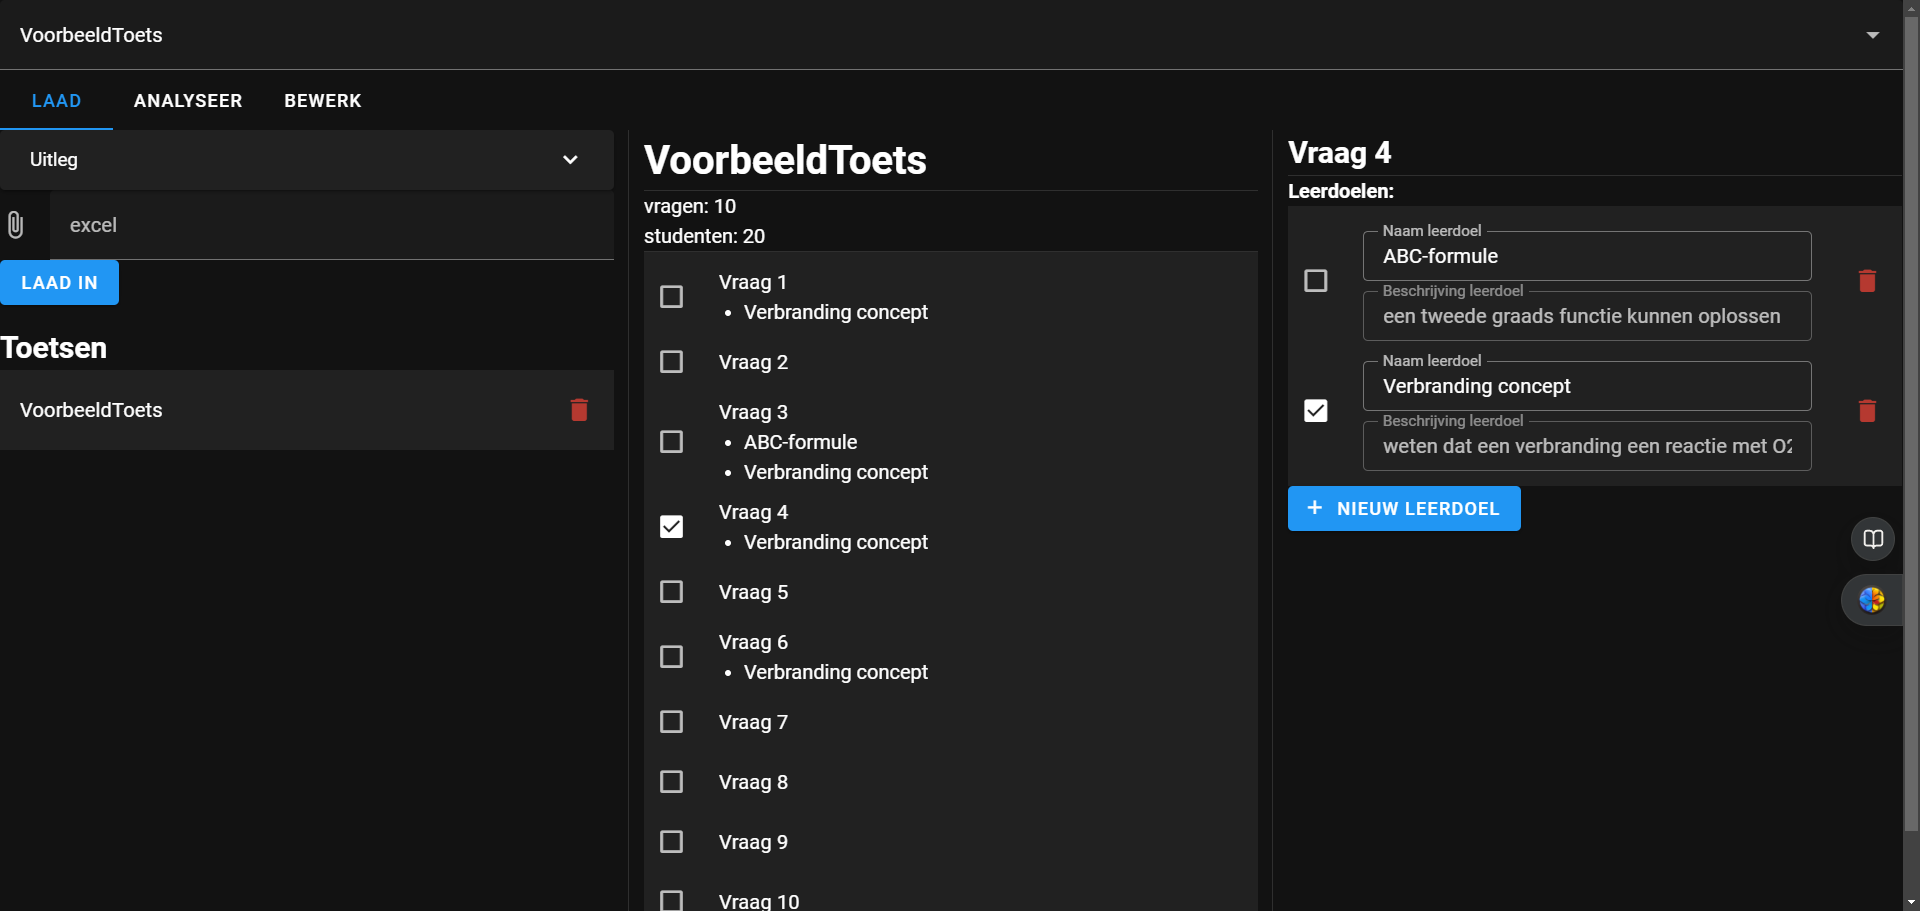
\includegraphics[width=1\linewidth]{./images/methoden/analyseren/ui/inlaad-pagina.png}
    \caption{Voorbeeld inlaadpagina}
    \label{fig:example-load-page}
\end{figure}
\noindent In het \textbf{analyse scherm} moet voor een docent overzichtelijk weergegeven zijn welke vragen goed en minder goed gingen en de scores van de leerlingen. Hier moet ook te zien zijn welke vragen waarschijnlijk niet thuishoren in de toets, omdat de mensen met een hoog cijfer hem fout hebben, dit kan komen dat die leerlingen te ver doordenken en daardoor de vraag fout hebben. De vraag is of je die leerlingen wilt afstraffen voor het verder denken dan het juiste antwoord. \\
\\
Het is ook mogelijk om hier opvallende correlaties tussen vragen weer te geven. Hier kan bijvoorbeeld worden laten zien dat mensen die vraag 5 fout hebben ook vraag 8 fout hebben. Dan is het mogelijk dat er 2x om dezelfde kennis wordt gevraagd, iets wat een toetsresultaat minder betrouwbaar maakt, omdat de stof disproposioneel wordt getoetst (dit geld ook voor een hoge correlatie tussen 2 juist gemaakte vragen). \\
\\
Het kan ook mogelijk zijn om de correlaties tussen leerlingen te tonen om eventuele spiekers te vangen. Hierbij moet wel rekening gehouden worden met het feit dat 2 mensen met een hoog cijfer, waarschijnlijk beide dezelfde vragen goed en fout hebben. Deze correlatie  wordt wel interessant bij bijvoorbeeld 2 6.5'en en precies dezelfde fouten.\\
\\
Op \textbf{het bewerkscherm} kunnen bijvoorbeeld een aantal velden komen met de doelen van een docent. Bijvoorbeeld: een veld om het gewilde gemiddelde en de gewilde standaarddeviatie in te stellen. Daarmee berekent hij dat een nieuwe formule. Hier kan ook worden of een lineare of non-lineare formule gebruikt wordt. Bij een non-lineare formule behoudt iedereen met een onvoldoende zijn onvoldoende, maar zijn die onvoldoendes minder hoog. \\
Hier kan ook op vraagniveau een scherm zijn om vragen eruit te gooien of half te laten meetellen, als blijkt dat ze wegnemen van de kennismeting van de toets.
\begin{figure}[H]
    \centering
    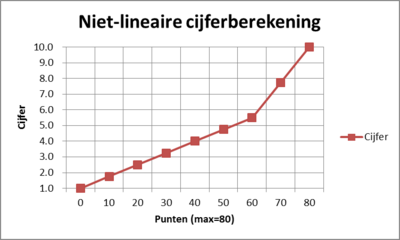
\includegraphics[width=1\linewidth]{./images/methoden/analyseren/Niet-lineaire.png}
    \caption{Non-lineair}
    \label{fig:non-linear}
\end{figure}
\begin{figure}[H]
    \centering
    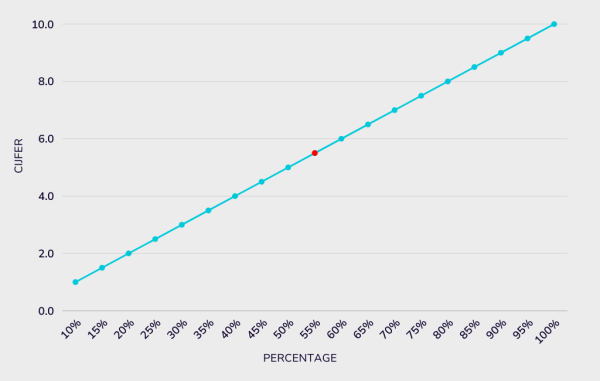
\includegraphics[width=1\linewidth]{./images/methoden/analyseren/linair.png}
    \caption{lineair}
    \label{fig:linair}
\end{figure}
\end{multicols}

\pagebreak
\subsection{Enquête}
\href{https://docs.google.com/spreadsheets/d/10Z6uwL6eRiDsPIC6HQ5hyizUN8RciJKFSDRZBGiKdDI}{resultaten}

\noindent
\begin{table}[H]
    \caption{Bent u bekend met het concept van (generatieve) AI? vs lesgeef ervaring}
    \begin{tabular}{l c c c c c}
        \toprule
        \textbf{Docent?} & \textbf{Ja} & \textbf{Gehoord} & \textbf{Nee} & \textbf{Totaal} \\
        \midrule
        1-5 jaar      & 4  & 4  &   &   & 8  \\
        5-10 jaar     & 5  & 4  &   &   & 9  \\
        Meer dan tien jaar & 13 & 16 & 1 &   & 30 \\
        Minder dan één jaar & 1  & 1  &   &   & 2  \\
        \midrule
        \textbf{Totaal} & 23 & 25 & 1 & 0 & 49 \\
        \bottomrule
    \end{tabular}
\end{table}

\noindent
\begin{table}[H]
    \caption{Bent u bekend met het concept van (generatieve) AI? vs vakgroep}

    \begin{tabular}{l c c c c}
        \toprule
        \textbf{Vakgroep} & \textbf{Op de hoogte} & \textbf{Ja} & \textbf{Nee} & \textbf{Totaal} \\
        \midrule
        alpha & 50.00\% & 50.00\% &  & 100.00\% \\
        beta  & 50.00\% & 42.86\% & 7.14\% & 100.00\% \\
        gamma & 28.57\% & 71.43\% &  & 100.00\% \\
        \midrule
        \textbf{Totaal} & 46.94\% & 51.02\% & 2.04\% & 100.00\% \\
        \bottomrule
    \end{tabular}
\end{table}

\noindent
\begin{table}[H]
\caption{Denkt u dat AI zelfstandig toetsen zou kunnen nakijken? vs lesgeef ervaring}
    \begin{tabular}{l c c c c}
        \toprule
        \textbf{Docent?} & \textbf{Ja} & \textbf{Nee} & \textbf{Weet niet} & \textbf{Totaal} \\
        \midrule
        1-5 jaar      & 37.50\% & 50.00\% & 12.50\% & 100.00\% \\
        5-10 jaar     & 44.44\% & 33.33\% & 22.22\% & 100.00\% \\
        Meer dan 10 jaar & 23.33\% & 40.00\% & 36.67\% & 100.00\% \\
        Minder dan 1 jaar &  & 50.00\% & 50.00\% & 100.00\% \\
        \midrule
        \textbf{Totaal} & 28.57\% & 40.82\% & 30.61\% & 100.00\% \\
        \bottomrule
    \end{tabular}
\end{table}

\noindent
\begin{table}[H]


    \caption{Denkt u dat AI zelfstandig toetsen zou kunnen nakijken? vs vakgroep}

    \begin{tabular}{l c c c c}
        \toprule
        \textbf{Vakgroep} & \textbf{Ja} & \textbf{Gehoord} & \textbf{Nee} & \textbf{Totaal} \\
        \midrule
        alpha & 28.57\% & 28.57\% &  & 57.14\% \\
        beta  & 14.29\% & 12.24\% & 2.04\% & 28.57\% \\
        gamma & 4.08\%  & 10.20\% &  & 14.29\% \\
        \midrule
        \textbf{Totaal} & 46.94\% & 51.02\% & 2.04\% & 100.00\% \\
        \bottomrule
    \end{tabular}
\end{table}

\noindent
\begin{table}[H]

    \caption{Denkt u dat AI zelfstandig toetsen zou kunnen nakijken? vs Bent u bekend met het concept van (generatieve) AI?}

    \begin{tabular}{l c c c}
        \toprule
        \textbf{AI Toetsen?} & \textbf{Ja} & \textbf{Gehoord} & \textbf{Nee} \\
        \midrule
        Ja      & 12.24\% & 16.33\% &  \\
        Nee     & 20.41\% & 18.37\% & 2.04\% \\
        Weet niet & 14.29\% & 16.33\% &  \\
        \midrule
        \textbf{Totaal} & 46.94\% & 51.02\% & 2.04\% \\
        \bottomrule
    \end{tabular}
\end{table}

\noindent
\begin{table}[H]
    \caption{Denkt u dat AI zelfstandig toetsen zou kunnen nakijken? vs vakgroep}

    \begin{tabular}{l c c c c}
        \toprule
        \textbf{Vakgroep} & \textbf{Ja} & \textbf{Nee} & \textbf{Weet niet} & \textbf{Totaal} \\
        \midrule
        alpha & 7  & 11 & 10 & 28 \\
        beta  & 4  & 5  & 5  & 14 \\
        gamma & 3  & 4  &    & 7  \\
        \midrule
        \textbf{Totaal} & 14 & 20 & 15 & 49 \\
        \bottomrule
    \end{tabular}
\end{table}

\noindent
\begin{table}[H]
    \caption{Hoeveel leerlingen trekken uw beoordeling per toets - terecht of niet - in twijfel? (Een getal) vs vakgroep}
    \begin{tabular}{l r r}
        \toprule
        \textbf{Vakgroep} & \textbf{Avg. twijfel} & \textbf{Aantal} \\
        \midrule
        alpha & 1.593 & 28 \\
        beta  & 2.000 & 14 \\
        gamma & 5.143 & 7 \\
        \midrule
        \textbf{Totaal} & 2.229 & 49 \\
        \bottomrule
    \end{tabular}
\end{table}

\noindent
\begin{table}[H]
    \caption{Wat zouden voor u redenen zijn om AI te gebruiken voor het nakijken van proefwerken? }
    \begin{tabular}{l c c c c c c}
        \toprule
        \textbf{Voordelen} & \textbf{Tijdsbesp.} & \textbf{Objectiv.} & \textbf{Werkdruk} & \textbf{Snelheid} & \textbf{Nauwk.} & \textbf{Nooit} \\
        \midrule
        \textbf{Totaal} & 40 & 14 & 31 & 18 & 8 & 7 \\
        \bottomrule
        \textbf{(\%)} & 80\% & 28\% & 62\% & 36\% & 16\% & 14\% \\
        \bottomrule
    \end{tabular}
\end{table}


\noindent
\begin{table}[H]
    \caption{Wat zijn uw belangrijkste zorgen bij het gebruik van AI voor het nakijken van proefwerken? }
    \begin{tabular}{l c c c c c c c}
        \toprule
        \textbf{Zorgen} & \textbf{Empathie} & \textbf{Tech. fout} & \textbf{Subjectiv.} & \textbf{Privacy} & \textbf{Bevoor.} & \textbf{Afhank.} & \textbf{Geen} \\
        \midrule
        \textbf{Totaal} & 20 & 26 & 31 & 11 & 11 & 15 & 0  \\
        \textbf{Totaal (\%)} & 40\% & 52\% & 62\% & 22\% & 22\% & 30\% & 0.00\% \\
        \bottomrule
    \end{tabular}
\end{table}

\paragraph*{De gemaakte punten in de resultaten van de open vraag.}

De vraag was: "Welke invloed denkt u dat de inzet van AI kan hebben op de relatie tussen docent en student?"

Voor het maken van deze lijst is voor het sorteren en overzichtelijk maken van de punten gebruik gemaakt van het GPT model Gemini Experimental 1121 op aistudio.google.com. Zie appendix voor prompt.

\begin{enumerate}
    \item \textbf{Negatieve invloed op de relatie en kennis van de docent}
        \begin{enumerate}
        \item Docent is minder goed op de hoogte van de inhoud van het leerlingwerk, wat informatie geeft over wat de leerling bezighoudt.
        \item Verminderd zicht op leerproces en denkstijl van de leerling.
        \begin{itemize}
        \item Docent kan sterke punten en ontwikkelpunten minder goed identificeren en hierop inspelen in de lessen.
        \item Docent mist mogelijk belangrijke informatie uit persoonlijke verhalen in schrijfopdrachten.
        \end{itemize}
        \item Docent voelt minder verantwoordelijkheid voor het nakijken en leerling kan moeilijker zijn recht halen.
        \item Minder intensief contact op niveau van interpretatie van antwoorden
        \item Docent moet mogelijk de AI-correctie zelf controleren, wat extra werk oplevert.
        \item Docent verliest mogelijk het zicht op de leercurve van de leerling.
        \item De professionele expertise van de docent wordt ondermijnd.
        \begin{itemize}
        \item Leerlingen kunnen denken dat docenten makkelijk vervangbaar zijn.
        \item Het werk van de docent kan in achting dalen bij leerlingen.
        \end{itemize}
    \end{enumerate}
\item \textbf{Afstand en verminderd persoonlijk contact}
    \begin{enumerate}
        \item   AI als nakijker of tutor kan de band minder persoonlijk maken.
        \item   Vervreemding tussen leraar en leerling en ten opzichte van zichzelf.
        \item    Verlies van menselijk contact en emotionele band, cruciaal voor effectief leren.
        \item   Dehumanisering van het onderwijs door rigide en onpersoonlijke AI-systemen.
        \item   AI kan leiden tot apathie bij de leerling.
        \item Relatie wordt anoniemer en onpersoonlijker.
        \item   Leerlingen zouden kunnen denken dat leraren niet essentieel zijn als AI ze kan vervangen.
    \end{enumerate}

\item \textbf{Discussie en twijfel over objectiviteit en correctheid}
    \begin{enumerate}
        \item   Discussies over de correctheid van AI-gegeven antwoorden en beoordelingen.
        \item   Leerlingen leren de subjectiviteit van zaken niet en dat niet alles zwart-wit is.
        \item Leerlingen zullen minder de neiging hebben om in discussie te gaan over de resultaten.
    \end{enumerate}

\item   \textbf{Potentieel positieve invloed, afhankelijk van de implementatie}
    \begin{enumerate}
        \item   AI kan de relatie versterken als docent en leerling samen leren AI te gebruiken voor oefenen, feedback en beoordelen.
        \item   Docent heeft meer tijd voor andere taken zoals het zoeken naar passend lesmateriaal.
        \item   Docent kan meer ontspannen zijn door vermindering van nakijkwerk.
        \item   AI kan een mediërende functie hebben door objectief vast te stellen of een antwoord fout is, waardoor docent en leerling zich kunnen richten op het 'waarom'.
        \item  AI kan voor leerling objectiever overkomen, waardoor minder snel gedacht wordt dat een punt niet gegund wordt door persoonlijke redenen.
        \item AI kan een suggestie van neutraliteit geven bij beoordeling.
        \item   AI kan bijdragen aan de relatie mits verstandig, met dat doel en openlijk ingezet.
        \item   Onderwijs kan beter worden afgestemd op individuele behoeften van leerlingen.
        \item Positieve invloed mits correct werkend.
    \end{enumerate}

\item   \textbf{Geen of weinig invloed}
    \begin{enumerate}
        \item   De relatie wordt voornamelijk bepaald door direct contact en hoe omgegaan wordt met discussies over beoordeling.
        \item   De relatie hoeft niet beïnvloed te worden.
        \item   AI kan het probleem van een tekort aan docenten oplossen.
        \item   Er is weinig ruimte voor AI om de relatie te verbeteren. Conflicten hebben vaak dieperliggende oorzaken dan meningsverschillen over nakijkwerk.
        \item   Geen invloed op de relatie.
        \item   Docent wil zelf verantwoordelijk blijven en met leerlingen in gesprek blijven.
    \end{enumerate}
    \item \textbf{Bezorgdheid over het gebruik van AI}
    \begin{enumerate}
        \item Zorgen over studenten die AI gebruiken om te schrijven en docenten die AI gebruiken om te controleren.
        \item   AI wordt verkeerd ingezet, zou alleen voor routineklussen gebruikt moeten worden.
        \item   AI wordt liever zoveel mogelijk buiten de deur en al helemaal uit het onderwijs gehouden.
    \end{enumerate}

\item   \textbf{Afhankelijkheid van het vak en type toets}
    \begin{enumerate}
        \item   Inzet van AI is afhankelijk van het vak; bijv. onhandig bij beeldende kunst, handig bij multiple choice.
        \item   Niet alle toetsen zijn geschikt voor AI, bijvoorbeeld de beoordeling van de schoonheid van een tekening of website.
    \end{enumerate}
\item   \textbf{Onzekerheid over de invloed}
\begin{enumerate}
     \item  Het is nog te vroeg om te zeggen wat de invloed zal zijn.
\end{enumerate}
\end{enumerate}

\pagebreak
\subsection{Praktijktest}
\begin{multicols}{2}
    

In dit gedeelte worden de resultaten van de afgenomen toets weergegeven. We beperken ons tot de beschrijving en interpretatie van de ruwe toetsresultaten, zonder hier nader in te gaan op de gebruikte beoordelingsmethode.

\subsubsection*{Verloop van de Afname}
De toets werd in een reguliere lesomgeving afgenomen, onder toezicht van de docent en ons. Alle leerlingen kregen 30 minuten de tijd om de toets te maken. Tijdens de afname deden zich geen noemenswaardige incidenten voor. De meeste leerlingen leverden hun antwoorden binnen de gestelde tijd in, en er waren geen signalen van technische problemen of externe afleiding. Deze omstandigheden suggereren dat de gemeten prestaties onder normale testcondities tot stand zijn gekomen.

In dit gedeelte worden de resultaten van de toets weergegeven. Deze cijfers zijn verkregen uit de automatisch verwerkte data (zonder hier in te gaan op hoe de AI dit heeft gedaan) en kunnen, afhankelijk van het verdere onderzoek, worden vergeleken met een menselijke beoordeling of andere referentiewaarden.

\subsubsection*{Algemeen Overzicht}
De toets bestond uit meerdere vragen, verdeeld over verschillende rubric-secties. Bij alle vragen is er sprake van enige variatie in de behaalde scores, zoals blijkt uit de standaarddeviaties.

\noindent In onderstaande tabel zijn per vraag het aantal deelnemers (N), het gemiddelde en de standaarddeviatie (SD) weergegeven. Daarnaast is het percentage leerlingen gegeven dat de vraag volledig goed (1 punt) heeft behaald. Omdat de vragen binaire scoring hebben (0 of 1), kun je de gemiddelde score interpreteren als het fractionele deel van leerlingen dat 1 punt heeft behaald.
\end{multicols}

\begin{table}[h!]
\centering
\begin{tabular}{llS[table-format=2.0]S[table-format=1.2]S[table-format=1.2]S[table-format=3.0]}
\toprule
\textbf{Rubric Sectie} & \textbf{Vraag} & \textbf{N} & \textbf{Gemiddelde} & \textbf{SD} & \textbf{\% 1-punt}\\
\midrule
1 & 1 & 23 & 1.00 & 0.00 & 100\\
1 & 2 & 22 & 0.09 & 0.29 & 9\\
1 & 3 & 23 & 0.48 & 0.51 & 48\\
1 & 4 & 22 & 0.64 & 0.49 & 64\\
1 & 5 & 20 & 0.75 & 0.44 & 75\\
1 & 6 & 21 & 0.86 & 0.36 & 86\\
1 & 7 & 19 & 0.11 & 0.32 & 11\\
\midrule
2 & 2 & 22 & 0.09 & 0.29 & 9\\
2 & 3 & 23 & 0.48 & 0.51 & 48\\
2 & 4 & 22 & 0.68 & 0.48 & 68\\
2 & 5 & 20 & 0.75 & 0.44 & 75\\
2 & 6 & 21 & 0.86 & 0.36 & 86\\
2 & 7 & 19 & 0.58 & 0.51 & 58\\
\midrule
3 & 4 & 22 & 0.55 & 0.51 & 55\\
\bottomrule
\end{tabular}
\caption{Overzicht resultaten per vraag. N = aantal leerlingen, Gemiddelde = fractie leerlingen met 1 punt, SD = standaarddeviatie, \% 1-punt = percentage leerlingen dat de sectie volledig goed beantwoordde.}
\end{table}

\pagebreak
\section{Conclusie}
\subsection{Inscannen}
\textbf{Vragen:}\\
\textbf{1. Welke manieren zijn er om een de vraagsecties op een foto te scheiden?} 
\begin{multicols}{2}
Van de 3 manieren die we hebben getest blijkt dat 1 methode onbruikbaar is en de andere 2 bruikbaar, maar in andere omstandigheden Tabel.\\
De methode die niet werkt is de kantlijnmethode. Het is niet mogelijk om ervan uit te gaan dat leerlingen alleen maar vraagnummers in de kantlijn zetten en daar alle secties op te baseren, want een kleine tekstherkennings fout kan antwoord op een vraag splitsen, waardoor iemand alle punten misloopt. \\
\\
De \textbf{QR-code} methode werkt goed voor werkbladen. Bijvoorbeeld een examen waar een leerling zo min mogelijk wil uitprinten. De leerling zou dan bijvoorbeeld een examenvraag uitprinten met daaronder direct het qr-antwoordveld, daar een foto van nemen die dan direct nagekeken wordt. 
\\
De \textbf{Checkbox} methode is de methode die het beste toepasbaar is voor een toets. Doordat er weinig/geen fouten worden gemaakt in het herkennen van een sectie, wat het doel is van deze deelvraag. Er is wel een leercurve voor de leerling. Na onze toets in de 3e klas blijkt dat die gymnasium 3 leerlingen er weinig moeite mee hadden, nadat wij het voordeden. Het kost een docent wel extra werk om tijdens het innemen van de toets te checken of iedereen op elk blaadje zijn id heeft opgeschreven. Bij ons toetsje waren er nog een aantal leerlingen die het nummer op de achterkant waren vergeten. Er was 1 sectienummer verkeerd ingelezen, maar dat soort errors kunnen gedetecteerd worden, door bijvoorbeeld te checken of deze leerling deze vragen misschien al een keer beantwoord heeft. Als dat zo is kan een docent met de hand checken welk leerling ID erbij past. 

% TODO: vergelijking met hypothese
\end{multicols}

\pagebreak
\noindent\textbf{2. Wat is de beste manier om tekst uit een ingescande sectie te halen?}
\begin{multicols}{2}
Uit de tests kunnen we ten eerste vaststellen dat de modellen van Google sneller zijn dan de modellen van OpenAI, zie:tabel \ref{fig:time-model}. Zoals verwacht zijn de flash modellen het snelst, maar we vonden het wel opvallend dat het verschil oploopt tot wel 3x sneller. \\
\indent We verwachtten dat het "nieuwste" model meestal de beste score zou hebben, maar dat is kennelijk niet helemaal waar, want de tekstherkenning van 1.5 pro heeft een betere gemiddelde score dan de gemini flash 2.0, die midden december 2024 is uitgekomen. Zie:tabel \ref{fig:score-model}. Dat is vooral te zien aan het gemiddelde aantal aanpassingen in een tekst, die bij flash 2.0 meer dan 2x zo groot is als 1.5 pro. Het (verwaarloosbare) nadeel is dat de standaarddeviatie van Gemini 1.5 pro meer dan 6x zo groot is als die van flash 2.0. \\
\indent Zoals we verwacht hadden geeft geeft een langere prompt een beter resultaat, zie:tabel \ref{fig:score-command}. Daarom hebben we ervoor gekozen om hiermee onze 3e klas toets in te scannen. \\
\indent Wat ons ook opviel is dat de context van de hele toets de beste inscanresultaten gaf, zie tabel \ref{fig:score-addition}. Wij hadden verwacht dat de rubric en de vraag de laagste (beste) score zou geven, maar het blijkt dat de toets de beste context geeft. Kennelijk begrijpen de modellen beter welke woorden iemand wil gebruiken als ze de hele toets hebben. Dat is ook te zien aan de gemiddelde veranderingen. Het is wel opvallend dat bij de rubric en de vraag geeft ook zo'n lage change count. De standaarddeviatie is daarentegen wel hoog, dus die combinatie is bij sommige vragen misschien beter dan de hele toets. Toch gaan we kiezen voor de vraag en antwoordmodel additie, want een hele toets zorgt voor een grote vermeerdering in tokens/kosten. Daarnaast neem de tijd per request toe.\\
\\
\noindent De opdracht die we gaan gebruiken:\\
\begin{tabularx}{\textwidth}{ll}
    \textbf{Model} & Gemini 1.5 pro 002 \\
    \textbf{Temperatuur} & 0.5 \\
    \textbf{Prompt} & lange uitleg bij elk veld \\
    \textbf{Additie} & vraag en antwoordmodel \\
\end{tabularx}

\end{multicols}
\pagebreak
\subsection{Nakijken}
\begin{multicols}{2}
Uit de resultaten blijkt dat grote taalmodellen in staat zijn om korte open scheikundevragen op tekstuele basis nauwkeurig na te kijken, met een correlatie die dicht in de buurt kan komen van menselijke beoordelaars. Er zijn echter aanzienlijke verschillen tussen de diverse geteste modellen en hun prestaties, met name wanneer we kijken naar de correlatiecijfers, de verschillen per vraag, en de frequentie van fout-positieven en fout-negatieven.

\paragraph*{Correlatie tussen Modellen en de Menselijke Beoordelaar} (Tabel "Correlatie modellen onder elkaar" \ref{fig:correlatie-model}):
De mens wordt als correcte grouden standaard gebruikt. De correlaties met het menselijke oordeel worden voor elk AI-model weergegeven. Gemini-2.0-flash-exp laat een zeer hoge correlatie zien met de menselijke beoordeling (rond de 0.95 en hoger). Deze sterke correlatie duidt erop dat deze modellen in veel gevallen vergelijkbaar beoordelen als een menselijke corrector, zeker bij eenvoudige, eenduidige open vragen.

Andere modellen, zoals “gemini-1.5-pro” en “gemini-1.5-flash”, tonen ook een sterke, maar iets lagere correlatie met de mens. Over het algemeen presteren alle getoonde modellen redelijk goed, met correlaties die vaak boven de 0.9 liggen. Dit geeft aan dat ze allemaal op tekstueel vlak redelijk in lijn liggen met de menselijke maatstaf, maar er zijn dus wel verschillen in nauwkeurigheid en consistentie.

\paragraph*{Verschil met Mens per Nagekeken Vraag} (Tabel “Verschil met mens per nagekeken vraag \%” \ref{fig:verschil-mens}):
Deze tabel geeft inzicht in de mate waarin de beoordeling van de modellen afwijkt van die van de menselijke beoordelaar, uitgesplitst per vraag. Hier zien we dat de meeste modellen bij vraag 1 vrijwel geen probleem hebben: sommige modellen tonen zelfs 0\% verschil met de menselijke beoordeling bij deze vraag. Dit is logisch omdat vraag 1 een multiple-choice vraag is.

Echter, het wordt interessanter bij andere vragen. Zo zien we bij meer complexe vragen vraag 5, de visueel-georiënteerde vraag met een foto of tekening dat het verschil met de mens ineens sterk toeneemt. Modellen die het bij tekstuele vragen goed deden, scoren bij vraag 5 duidelijk minder. Dit duidt erop dat modellen moeilijkheden ondervinden als niet puur tekstuele interpretatie vereist is. De verschillen van ruim boven de 10\% geven aan dat de AI hier echt niet op het niveau van een mens presteert.

Samenvattend illustreert deze tabel dat AI-modellen uitblinken in standaard, tekstuele en eenduidige vragen. Alleen nog wel zwakker zijn bij complexere en visuele vragen. Elk model heeft zo zijn eigen profiel: sommige zijn beter in standaardvragen, andere houden zich iets beter staande bij complexere vragen, maar geen enkel model evenaart de mens volledig op het visuele vlak.

\paragraph{Aantal Valse Positieven en Aantal Valse Negatieven} (Tabel “Aantal valse positieve en aantal valse negatieve” \ref{fig:false-pos-neg}):
De laatste tabel toont ons in detail wanneer het model ten onrechte punten toekent (false positive) of ten onrechte aftrekt (false negative) ten opzichte van de menselijke beoordeling. Een false positive betekent dat de AI een leerling te veel krediet geeft voor een antwoord dat volgens de mens niet correct is. Een false negative betekent dat de AI punten aftrekt terwijl de mens dit niet zou doen, dus de leerling wordt hier strenger beoordeeld.

Hier zien we bijvoorbeeld dat “gemini-2.0-flash-exp” niet altijd gelijkmatig presteert. Bij bepaalde vragen ontstaan meerdere false positives of false negatives, wat in totaal tot 15 of meer incorrecte oordelen kan leiden als we dit over de gehele set bekijken.

Opvallend is dat de complexere vragen niet alleen leiden tot een hoger percentage afwijking, maar ook tot meer onjuiste beoordelingen in termen van false positives en false negatives. Dit betekent dat de AI niet alleen anders scoort dan de mens, maar dat die afwijking in sommige gevallen systematisch kan zijn (bijvoorbeeld consequente overschatting van een bepaalde fout of onderschatting van een bepaald correct element).

\paragraph{Relatie tot Menselijke Beoordeling en Hybride Aanpak}
De tabellen samen suggereren dat voor standaard open vragen, vooral wanneer het antwoord eenduidig en tekstueel is, AI-modellen erg dicht bij de menselijke beoordeling kunnen komen. Dit biedt perspectief op grootschalige inzet voor eerste selecties, voorbeoordelingen of als tijdbesparend instrument bij het nakijken. Echter, voor complexere taken (bijvoorbeeld vragen die berusten op visuele interpretaties, subtiele chemische notaties, of context-specifieke nuances) blijft er een duidelijk gat. Deze kloof uit zich in verhoogde verschillen per vraag en een hoger aantal false positives en false negatives.

De bevindingen tonen hiermee de noodzaak van menselijk toezicht. Hoewel AI de potentiële efficiëntie en consistentie kan verhogen, is menselijke interventie nodig om complexere, visuele of dubbelzinnige gevallen correct te beoordelen. Een hybride aanpak, waarin menselijke beoordelaars en AI-systemen samenwerken, lijkt hierdoor de optimale strategie. De mens kan zich dan richten op de lastige, subtiele of visuele aspecten, terwijl de AI het grote aandeel van de standaard vragen snel en consistent verwerkt.

\paragraph*{Algemene Conclusie}
De verschillen tussen de modellen zijn subtiel maar betekenisvol: sommige modellen hebben een hogere correlatie met de menselijke beoordeling, andere hebben een lagere frequentie van valse positieven of negatieven. Bij eenvoudige, eenduidige tekstuele vragen kunnen de beste modellen bijna even goed of zelfs even goed als een mens scoren. Bij complexere vraagtypes, waaronder visuele of notatiegevoelige taken, zien we echter een duidelijke terugval in nauwkeurigheid en betrouwbaarheid.

Kortom, AI-systemen zijn een waardevolle aanvulling op, maar (nog) geen vervanging voor menselijk nakijken. De resultaten tonen een duidelijke meerwaarde voor tijdsbesparing en consistentie, maar ook de blijvende noodzaak van menselijke expertise bij complexe of visueel-gedreven examenonderdelen.


\end{multicols}
% TODO: checken of dit enin moet blijven
% \subsection{Analyseren}
% \begin{multicols}{2}

% Naast bekende statistische maten als gemiddelde, standaarddeviatie en covariantie, zijn op vraagniveau de Item-Rest Correlatie (RIR) en Item-Totaal Correlatie (RIT) toegepast om de bijdrage van individuele vragen aan de totale score te beoordelen. Deze visulizaties zijn gemaakt m.b.v Google Gemini 1.5 pro.

% Een voorgestelde gebruikersinterface (UI) met een input-, analyse- en bewerkscherm faciliteert de praktische toepassing. 
% \noindent\begin{itemize}
%     \item \textbf{Input:} Toetsresultaten uploaden en leerdoelen koppelen.
%     \item \textbf{Analyse:} Prestaties op vraag- en leerlingniveau, inclusief correlaties.
%     \item \textbf{Bewerking:} Gewenst gemiddelde/standaarddeviatie instellen, vragen aanpassen.
% \end{itemize}
% \end{multicols}

\pagebreak
\subsection{Enquete}
\begin{multicols}{2}
Uit de resultaten van de enquête komt naar voren dat er onder docenten een redelijk goede bekendheid is met het concept van (generatieve) AI, maar dat de mate van bekendheid en de perceptie van mogelijke inzet ervan varieert. Er zijn duidelijke verschillen waarneembaar tussen docenten met uiteenlopende leservaring en vakgroepsachtergronden. 

Allereerst laat de data zien dat docenten met meer onderwijservaring niet per definitie bekender zijn met AI-concepten dan docenten met minder ervaring. Bovendien zijn meningen over de potentiële inzet van AI voor het nakijken van toetsen verdeeld. Docenten met kortere werkervaring lijken iets positiever te staan tegenover de mogelijkheid dat AI zelfstandig kan corrigeren, terwijl docenten met meer dan tien jaar ervaring terughoudender zijn. 

Er zijn eveneens verschillen tussen vakgroepen te onderscheiden. Docenten uit de ‘gamma’-groepen lijken minder vaak op de hoogte te zijn van generatieve AI dan docenten uit ‘alpha’- en ‘beta’-richtingen. Tegelijkertijd blijkt ook het aantal leerlingen dat toetsbeoordelingen in twijfel trekt te verschillen per vakgroep, waarbij docenten uit de ‘gamma’-groep aangeven dat hun beoordeling gemiddeld vaker in twijfel wordt getrokken dan vakgroepen. 

Als verwachtte voordelen wordt vooral tijdsbesparing, objectiviteit, en het verminderen van de werkdruk genoemd als motivatie om AI in te zetten voor het nakijkproces. Belangrijke zorgen betreffen echter de subjectiviteit van AI, mogelijke technische fouten en een verminderd empathisch vermogen. De angst dat het menselijk, relationeel aspect van onderwijs verloren gaat, komt hierbij naar voren. Er bestaan zorgen dat docenten minder voeling krijgen met het individuele leerproces van leerlingen, en dat door toenemende inzet van AI de persoonlijke relatie tussen docent en leerling kan verzwakken. 

Tegelijkertijd zijn er ook meer genuanceerde of positieve verwachtingen. Sommige docenten geven aan dat AI, mits verantwoord geïmplementeerd, de relatie kan verbeteren. Dit komt doordat docenten meer tijd vrijspelen voor persoonlijke begeleiding. Daarnaast kan AI zorgen voor een objectievere en transparantere beoordeling. Hierdoor ontstaat er minder discussie over puntenaantallen. Tot slot is er een groep die denkt dat AI weinig tot geen invloed zal hebben. Zij geloven dat menselijk contact en interactie blijven domineren.

Kortom, de bevindingen tonen een verdeeld landschap. Docenten zijn zich meer bewust van AI. Ze zien voordelen op het gebied van efficiëntie en objectiviteit. Tegelijkertijd uiten ze zorgen over verlies aan menselijkheid en verminderde professionele autonomie. Ook vrezen ze een afname van diepgaand contact met leerlingen. De uiteindelijke invloed hangt sterk af van de wijze waarop AI wordt ingezet. Belangrijk is dat docenten hun professionele beoordelingsvermogen blijven benutten. Daarnaast moet de relatie met de leerling persoonlijk en ondersteunend blijven.
\end{multicols}
\pagebreak
\subsection{Praktijktest}
Op basis van de bovenstaande resultaten zijn enkele observaties en mogelijke conclusies te trekken:

\noindent\begin{itemize}
    \item \textbf{Makkelijke vragen:} De resultaten voor Rubric Sectie 1, Vraag 1 (Gemiddelde: 1.00, SD: 0.00) tonen aan dat alle leerlingen deze vraag probleemloos beantwoordden. Ook voor de vragen 5 en 6 in zowel Sectie 1 als Sectie 2 liggen de gemiddelde scores rond of boven de 0.75 met relatief lage spreiding, wat suggereert dat deze onderwerpen goed worden begrepen.
    
    \item \textbf{Moeilijke vragen:} De zeer lage gemiddelde scores voor Vraag 2 in Sectie 1 en Sectie 2 (beide Gemiddelden: 0.09) en Vraag 7 in Sectie 1 (Gemiddelde: 0.11) duiden erop dat deze vragen als moeilijk of onduidelijk werden ervaren door de leerlingen. De geringe spreiding (relatief lage standaarddeviatie in vergelijking met de gemiddelde score) bij deze vragen suggereert dat vrijwel niemand op deze onderdelen goed scoorde.
    
    \item \textbf{Heterogene resultaten:} Bij vragen met gemiddelde scores rond de 0.5 en een standaarddeviatie rond 0.5, zoals Vraag 3 en Vraag 4 in meerdere rubric-secties, is sprake van een grote variatie in de prestaties. Dit kan betekenen dat sommige leerlingen de gevraagde vaardigheden of kennis goed beheersen, terwijl anderen er duidelijk moeite mee hebben.
    
    \item \textbf{Consistentie tussen rubric-secties:} Sommige vragen (bijvoorbeeld Vraag 4 en 5) vertonen vergelijkbare gemiddelde en spreidingspatronen in verschillende rubric-secties, wat kan wijzen op een stabiele moeilijkheidsgraad. Daarentegen levert Vraag 7 in Sectie 2 (Gemiddelde: 0.58) significant betere resultaten op dan in Sectie 1 (Gemiddelde: 0.11), wat zou kunnen duiden op een verschil in context, formulering, of voorkennis.
    
    \item \textbf{Aanbevelingen:}  
    De resultaten suggereren dat bepaalde concepten of vaardigheden (zoals die in Vraag 2 en Vraag 7, Sectie 1) extra aandacht nodig hebben in de lespraktijk. Verder kunnen docenten overwegen om de formulering of instructies bij de moeilijkere vragen aan te scherpen om leerlingen beter voor te bereiden of te ondersteunen.
\end{itemize}

Samengevat geeft de data inzicht in welke onderdelen van de leerstof leerlingen goed of minder goed beheersen en kunnen deze resultaten als basis dienen voor verdere verbeteringen in de toetsing en de didactische aanpak.
\pagebreak
\section{Demo}
\subsection{Opzet}
Online hebben we een demo op: \href{https://toetspws.web.app/}{https://toetspws.web.app/}\\
Wij vonden het belangrijk dat de docent 100\% controle heeft over een toets. Dus elk tekstveld is aanpassbaar, zodat een fout van AI altijd aangepast kan worden. \\
Ook kunnen docenten zelf bepalen welk model en provider voor alles wordt gebruikt, om te testen welke het beste werkt. Sommige modellen werken niet voor elke feature.
\\
Hieronder is informatie te vinden over hoe deze site werkt en hoe hij gebruikt kan worden.\\
\begin{figure}[H]
    \centering
    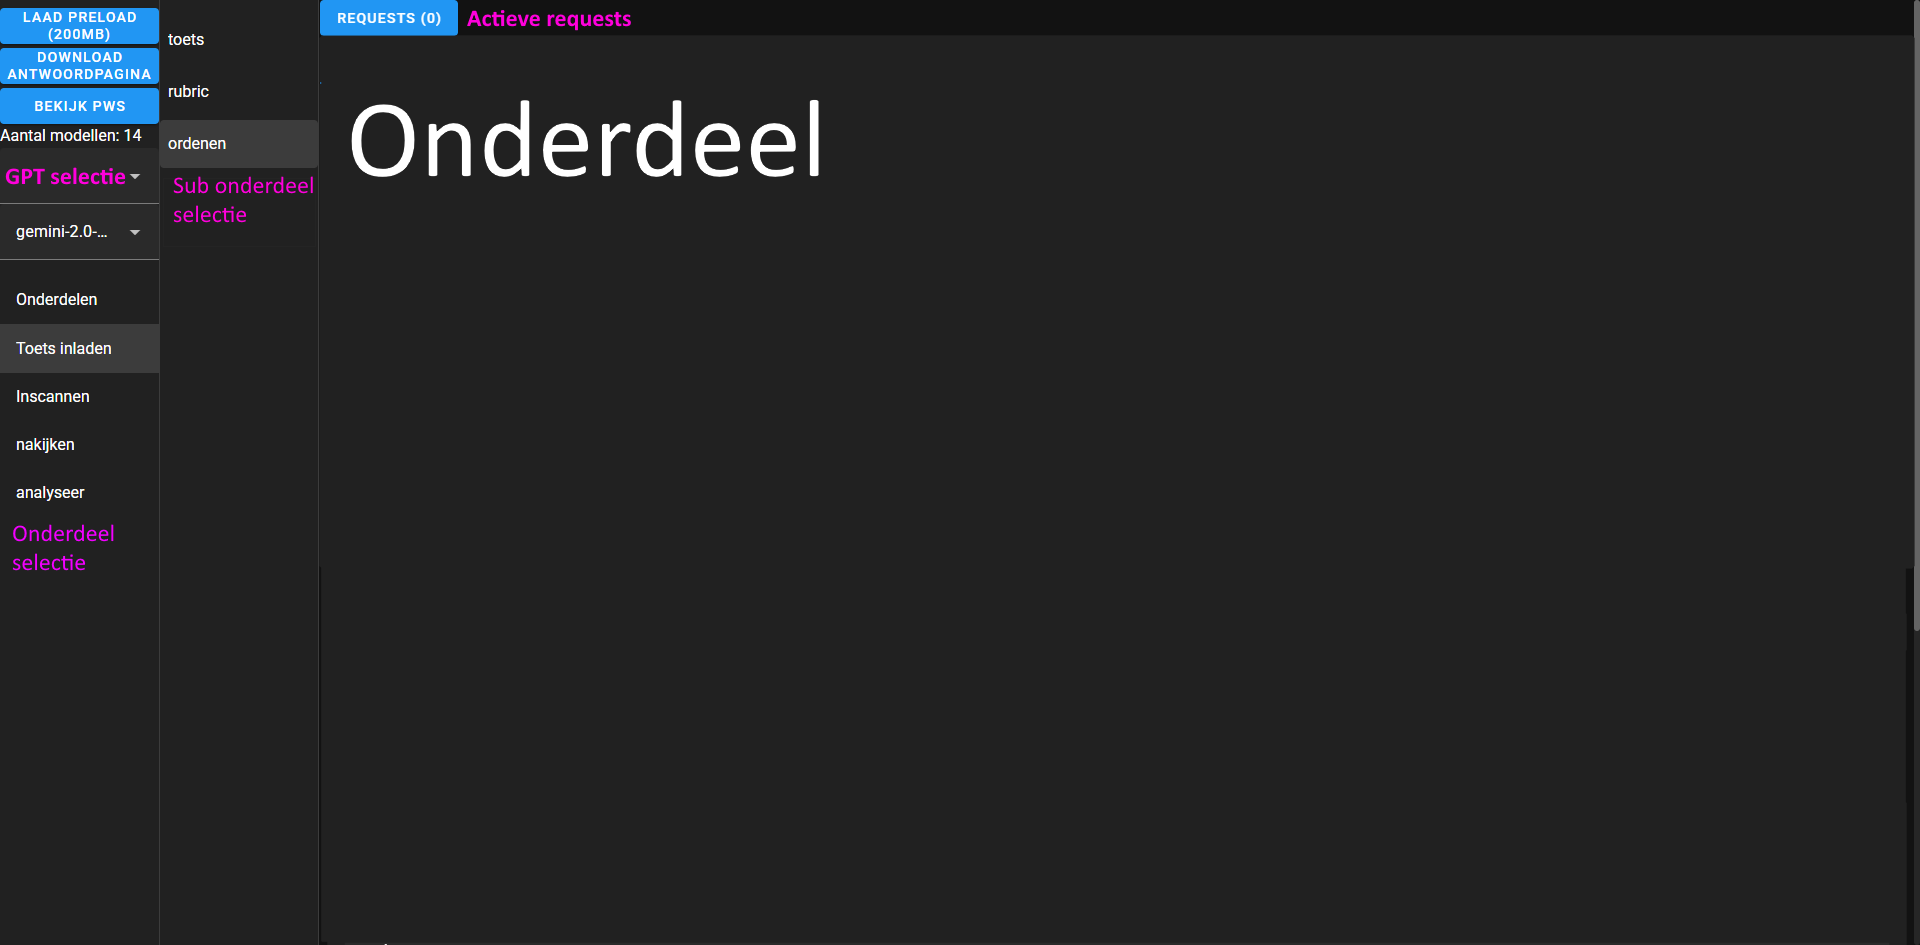
\includegraphics[width=\linewidth]{./images/demo/overview.png}
    \caption{Overview site}
    \label{fig:demo-overview}
\end{figure}

\noindent Hier kan een docent zien wat er nu bezig is en kan alles stoppen als iets te lang duurt of als hij iets wilt aanpassen.
\begin{figure}[H]
    \centering
    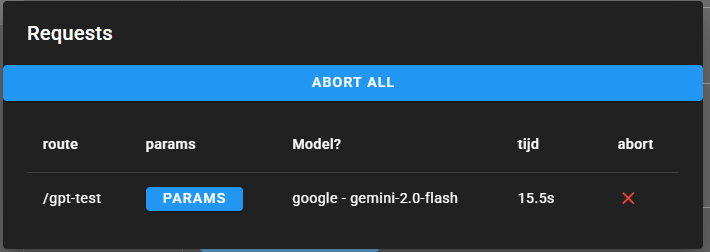
\includegraphics[width=\linewidth]{./images/demo/requests.png}
    \caption{Request Manager}
    \label{fig:request-manager}
\end{figure}

\begin{figure}[H]
    \centering
    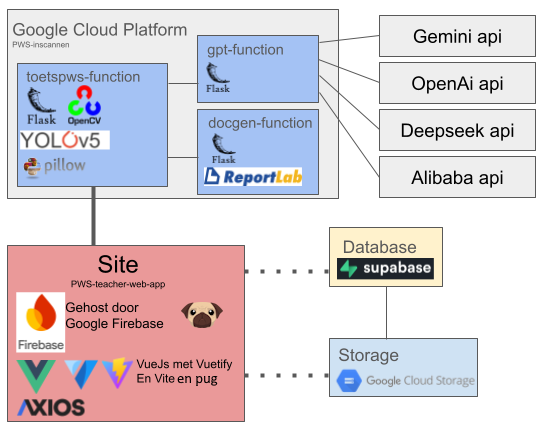
\includegraphics[width=\linewidth]{./images/demo/stack.png}
    \caption{Techstack}
    \label{fig:tech-stack}
\end{figure}

\pagebreak
\subsection{Toets omzetting/generatie}

Toetsen hebben vragen en leerdoelen, zodat de docent aan het einde kan zien welke leerdoelen wel en niet behaald zijn. Ook is elk punt gekoppelt aan een leerdoel, deze worden automatisch gegenereerd.\\
Er zijn 2 methodes om een toets in te laden:\\
\begin{itemize}
    \item Upload: gooi de pdf en rubric van de toets in de file uploaders. Selecteer het onderdelen menu en laad de structuur in. Het geselecteerde gpt model zal de tekst en foto's uit die pdf's omzetten naar een toets model.
    \item Toets generatie mbv AI. Vul informatie over de toets die je wilt geven in in het menu. Nakijkregels gaan er later voor zorgen dat de dingen die een docent automatisch doet en niet in de rubric staan toch worden meegenomen in de beoordeling. Dit kost ongeveer 30s.
\end{itemize}
\begin{figure}[H]
    \centering
    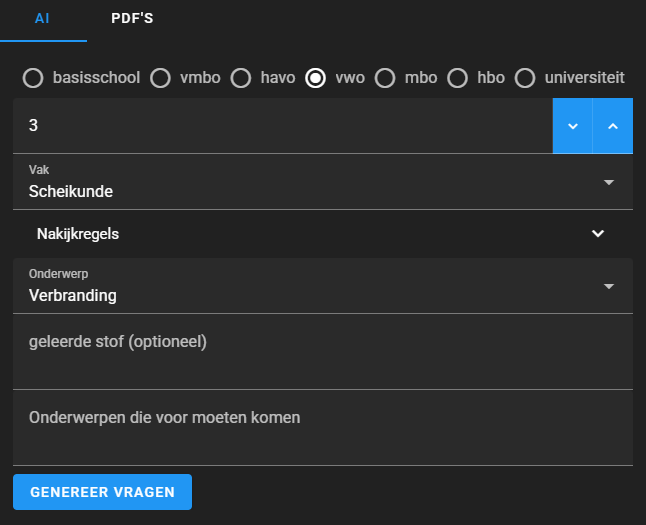
\includegraphics[width=\linewidth]{./images/demo/generation/settings.png}
    \caption{Gpt settings}
    \label{fig:gpt-gen-settings}
\end{figure}
\pagebreak
\paragraph{Printen} Print de toets daarna naar docx of pdf. De meeste tekstvelden hebben support voor markdown en latex formules tussen dollar tekens. Dit werkt ook in de output naar docx. Zie \href{https://github.com/TanteJossa/PWS-inscannen/tree/main/flask_apps/doc_gen}{doc-gen-git}.
\begin{figure}[H]
    \centering
    \includegraphics[width=\linewidth]{./images/demo/generation/word.png}
    \caption{Word output met formules}
    \label{fig:word-gen}
\end{figure}

\subsection{Inscannen}
Docenten kunnen de foto's van de de toetsblaadjes per stuk fotograferen en importeren, of een ingescande pdf uit een printen uploaden. Daarna kunnen de foto laten uitsnijden (als de foto met een telefoon is gemaakt) en de rode pen weghalen als het al is nagekeken. Ook kunnen gedraaide fotos geflipt worden en lege pagina's verwijderd.
\begin{figure}[H]
    \centering
    \includegraphics[width=\linewidth]{./images/demo/scanning/load.png}
    \caption{Antwoorden inladen}
    \label{fig:load-student-pdf}
\end{figure}
Daarna kan worden de secties herkent en de vraagnummers herkent.
\begin{figure}[H]
    \centering
    \includegraphics[width=\linewidth]{./images/demo/scanning/checkbox.png}
    \caption{Vraag sectie herkenning}
    \label{fig:scan-checkbox}
\end{figure}
Daarna kan een docent automatisch de tekst inladen van elke vraag van elke leerling. Dit kan in bulk of per vraag.
\begin{figure}[H]
    \centering
    \includegraphics[width=\linewidth]{./images/demo/scanning/text.png}
    \caption{Vraag text herkenning}
    \label{fig:scan-text}
\end{figure}

\pagebreak
\subsection{Nakijken}
Daarna kan een docent de toets laten nakijken. De modellen geven feedback op elk punt, waardoor een leerling er meer aan heeft. Ook kijkt hij naar verbeterpunten, ookal is een antwoord goed (zie voorbeeld).
\begin{figure}[H]
    \centering
    \includegraphics[width=\linewidth]{./images/demo/grading/grade.png}
    \caption{Nakijken}
    \label{fig:grade-result}
\end{figure}
\pagebreak
\subsection{Analyseren/terugkoppeling gebruiker}
Er is terugkoppeling voor de docent en voor de leerling. Een docent kan per leerling (of allemaal tegelijk) een pdf uitprinten met daarin de resultaten van de toets en feedback. Ook krijgt een leerling te zien welke leerdoelen goed en minder goed gaan.
\begin{figure}[H]
    \centering
    \includegraphics[width=\linewidth]{./images/demo/analisys/question.png}
    \caption{Resultaat per vraag per leerling}
    \label{fig:result-per-question}
\end{figure}
\begin{figure}[H]
    \centering
    \includegraphics[width=\linewidth]{./images/demo/analisys/target.png}
    \caption{Resultaat per leedoel}
    \label{fig:result-per-target}
\end{figure}
\pagebreak
Ook kunen docenten een overview krijgen van alle resultaten.
\begin{figure}[H]
    \centering
    \includegraphics[width=\linewidth]{./images/demo/analisys/overview.png}
    \caption{Overview}
    \label{fig:teacher-overview}
\end{figure}
\pagebreak
\subsection{Vervolg}
\begin{itemize}
    \item In het vervolg zouden we een database achter de site kunnen zetten, zodat docenten toetsen en resulaten kunnen opslaan om later mee verder te gaan. Ook zouden docenten dan hun toetsen publiek kunnen maken, zodat andere docenten de resultaten kunnen bekijken. 
    \item Toetsen uitbreiden zodat die ook foto's kunnen hebben in zowel de antwoorden als in de vraag/context van de vraag.
\end{itemize}
\noindent Een deel van deze ideeën zijn in de "database" branch te vinden (\href{https://github.com/TanteJossa/PWS-teacher-web-app/tree/database}{database branch}) 
\begin{figure}[H]
    \centering
    \includegraphics[width=\linewidth]{./images/demo/browser.png}
    \caption{Zoekfunctie/toetsen opslaan}
    \label{fig:browser-preview}
\end{figure}


\pagebreak
\section{Discussie}
\subsection{Foutenanalyse}
\begin{multicols}{2}
\noindent\begin{minipage}{\linewidth}
    
\subsubsection{Inscannen}
$\bullet$ Tijdens het testen van instellingen zijn er een aantal gefaald, omdat er te veel requests per seconde werden gestuurd. Dit kan ervoor hebben gezorgd dat de resultaten verdraaid zijn.\\
$\bullet$ Er kan meer getest worden met de ideale prompt die een beter resultaat geeft. \\
$\bullet$ Tijdens het toetsje zijn een aantal vragen verkeerd ingescand, omdat een leerling de checkbox verkeerd had ingevuld. Het zou netter zijn om dit als een popup aan een docent te laten zien die dit dan corrigeert.\\
\end{minipage}

\noindent\begin{minipage}{\linewidth}
\subsubsection{Nakijken}
$\bullet$ \textbf{Complexe, visuele vragen zijn een uitdaging:} Meer fout-positieve en fout-negatieve beoordelingen, vooral bij handgetekende structuren, schema's en grafische voorstellingen.\\
$\bullet$ \textbf{Inscannen kan ook fouten geven:} Het is mogelijk dat fouten door het inscannen van de vragen komen, en niet door de AI.\\
$\bullet$ \textbf{Verschillen tussen modellen:} De meeste modellen presteren vergelijkbaar met andere benchmarks, maar \textbf{o1-mini} presteert slechter bij visuele vragen.\\
$\bullet$ \textbf{Verbeterpunten:}\\
\begin{minipage}{0.9\linewidth}
\hspace{3em}$\bullet$ \textbf{Fine-tuning:} Trainen op chemische datasets met visuele representaties.\\
\hspace{3em}$\bullet$ \textbf{Promptoptimalisatie:} Betere prompts en consistentiecontroles.\\
\hspace{3em}$\bullet$ \textbf{Mens-AI samenwerking:} AI voor eenvoudige vragen, mens voor complexe vragen.
\end{minipage}
\end{minipage}
\begin{minipage}{\linewidth}
\subsubsection{Analyseren}
$\bullet$ De bedachte UI is niet getest, waardoor er niet een 2e iteratie verbeteringen is gedaan.\\
$\bullet$ We hebben geen echte toetsen geanalyseerd, omdat de toets die we zouden krijgen zo slecht gemaakt was dat er niets te analyseren was.\\
$\bullet$ Tijdens het toetsje zijn een aantal vragen verkeerd ingescand, omdat een leerling de checkbox verkeerd had ingevuld. Het zou netter zijn om dit als een popup aan een docent te laten zien die dit dan corrigeert.\\
\end{minipage}
\begin{minipage}{\linewidth}

\subsubsection{Enquête}
$\bullet$ We kregen terug van een aantal docenten dat de vraag aantal leerlingen die het oneens is met een beoordeling niet exact gedefineerd was.\\
$\bullet$ Er waren relatief weinig gamma resultaten, waardoor hun reactie statistisch gezien minder waarde heeft.\\
$\bullet$ Dit is een enquête gestuurd naar docenten van Het Amsterdams Lyceum en hiermee kunnen we nog weinig zeggen over of docenten in de rest van Nederland andere problemen hebben.\\
\end{minipage}
\begin{minipage}{\linewidth}
\subsubsection{Praktijktest}
$\bullet$ We hebben dit toetsje afgenomen bij een hele lieve gymnasium klas. Het is de vraag op andere klassen andere manieren vinden om het blaadje zo toe te takelen dat het nakijkprocess wordt verhinderd.\\
\end{minipage}
\begin{minipage}{\linewidth}
    
\subsection{vervolgonderzoek}
$\bullet$ Een onderzoek/test naar een interface die docenten kunnen gebruiken om de inscan en nakijk modules makkelijk tegebruiken\\
$\bullet$ Een onderzoek naar wat docenten op andere scholen belangrijk vinden\\
$\bullet$ Een onderzoek naar wat docenten van ons de resultaten van ons toetsje vinden en of dit hun mening verandert over de mogelijkheden van nakijken met AI\\
$\bullet$ Een onderzoek naar hoe zo'n systeem geïntegreerd kan worden in het huidige onderwijs. Denk hierbij aan het printen van de custom toetsblaadjes of het omzetten van huidige toetsen naar een computerformat  die een ai kan gebruiken.\\
$\bullet$ De avond voor het inleveren van dit PWS heeft Google een nieuw model gelanceerd: \textbf{Gemini 2.0 flash thinking experimental} dat model bedenkt eerst een stappenplan voordat hij iets gaat uitvoeren. Het jammer dat dit net te laat is om in ons onderzoek mee te nemen, maar uit een paar test zijn de resultaten zeer positief voor tekstuele en visuele vragen. (een redox reactie herkennen en uitleggen). Naar dit model kan ook onderzoek gedaan worden.\\
\end{minipage}
\end{multicols}
\pagebreak

\subsection{Terugblik en dankwoord}
\begin{multicols}{2}
\noindent\begin{minipage}{\linewidth}
    
\paragraph*{Reflectie Joost} Dit project heb ik veel geleerd over het overstappen naar een andere methode. Voor de inscanmodule had ik in het begin ingeschat dat ik maar 10 uur nodig had voor het inscannen. De daadwerkelijke tijd was een stuk meer. De methode die ik had bedacht (tekstherkenning in de kantlijn) bleek niet te werken, maar ik heb wel (onnodig) veel tijd besteed aan het optimaliseren van dat proces. Ik heb ook veel gehad aan het gebruiken van de Google Gemini API, die gebruik ik nu vaak om kleine simpele taakjes op te lossen. Ook heb ik Google Sheets pivot tables leren gebruiken om snel de enquete, inscan en toets resultaten in tabellen te zetten (die ik daarna met Google Gemini naar de latex/pdf tabellen heb omgezet). Het inscan en nakijksysteem zal ik waarschijnlijk in een ander project gaan gebruiken. Waar volgend jaar misschien rekening mee gehouden kan worden is dat de rubrics van het PWS niet duidelijk de opdracht van het PWS weerspiegelen. Tot fase 3 is eigenlijk literatuuronderzoek en een paar beantwoorde deelvragen. Fase 4 is het onderdeel waar je het "grote" onderzoek moet uitvoeren. Ik vond dat we die fase pas laat kregen en dat er dingen misten in de rubric die ik wel verwacht in een wetenschappelijk onderzoek (bijvoorbeeld de indeling of het hebben van resultaten). Ik zie dit PWS meer als een eigen project dan als een opdracht voor school en eigen projectjes vind ik leuk om te doen, zie: \href{https://github.com/TanteJossa}{Mijn Github}.  
\end{minipage}
\begin{minipage}{\linewidth}
\paragraph*{Reflectie Jonathan} Tijdens dit project heb ik een scheikundetoets gemaakt en een nakijksysteem ontwikkeld. 
Ik heb hierbij veel geleerd over het gebruik van technologie om processen makkelijker en sneller te maken. \\
In het begin dacht ik dat het nakijken van de toets vrij simpel zou zijn, maar uiteindelijk bleek het toch lastiger dan verwacht. 
Vooral het opzetten van de automatische correctie kostte meer tijd, omdat ik veel moest testen om te zorgen dat alles goed werkte.\\

Een belangrijk onderdeel van het project was het gebruik van API requests naar OpenAI.
Hiermee kon ik data sturen en automatisch antwoorden of feedback ontvangen, wat het nakijksysteem efficiënter maakte.
Ik leerde hoe ik de API kon aanroepen en de resultaten kon verwerken, wat ik erg handig vond. Dit was de eerste keer dat ik met API’s werkte 
en het heeft me laten zien hoe krachtig en flexibel ze kunnen zijn voor dit soort taken.\\

Daarnaast heb ik veel tijd besteed aan het testen van variabelen in het nakijksysteem.
Door kleine aanpassingen te doen en telkens opnieuw te testen, kon ik het nakijkproces steeds een beetje beter maken.
Dit was soms best frustrerend, omdat het niet altijd meteen werkte.
Uiteindelijk was het het toch waard toen het systeem op z'n best werkte.\\

Dit project heeft me laten zien hoe technologie kan helpen bij het automatiseren van taken zoals nakijken.
Ik vond het leuk om te zien hoe het stukje bij beetje in elkaar viel.
Als ik dit project vergelijk met andere schoolopdrachten, voelde het meer als een eigen project waar ik echt zelf de controle over had.
Hierdoor vond ik het ook leuker en heb ik veel geleerd, bijvoorbeeld over API’s en het testen van systemen.
Ik denk dat ik de kennis die ik nu heb opgedaan in toekomstige projecten zeker ga gebruiken!
\end{minipage}
\paragraph*{Dankwoord} 
Dit project hebben we niet alleen kunnen doen. Als eerste willen we graag onze begeleider, \textbf{Philip Hermarij}, bedanken voor het mogelijk maken van onze praktijktest. Daarnaast vonden we het fijn dat hij ons liet concentreren op het maken van het systeem, in plaats van ons achterna zitten met de opdracht en rubric.\\
\noindent\begin{minipage}{ \linewidth}
Daarnaast willen we graag \textbf{Deirdre Vos} bedanken voor 2 dingen:
\noindent\begin{itemize}
    \item  Het ondersteunen van het analyseer onderzoek, door ons geanonimiseerde toetsresultaten te geven. Daarnaast heeft ze ook input gegeven voor wat haar handig lijkt in een mogelijke interface, zoals het toewijzen van rubricpunten aan leerdoelen. Ook hebben de lessen wiskunde D over statistiek en kansen ons geholpen in het analyseren van de toets enquête en nakijkresultaten\\
    \item Ons in contact brengen met Daniël Markus. 
\end{itemize}
\end{minipage}
Bij \textbf{Daniël Markus} hebben we een interview afgenomen over gebruik van AI voor het nakijken en inscannen. Bij dat interview was een onderzoeken naar AI die ons ook belangrijke inzichten heeft gegeven, bijvoorbeeld voor de checkbox inscanmethode.\\
\\
Als laatste willen we alle \textbf{docenten} die tijd hebben genomen om onze enquête in te vullen  bedanken. We konden daardoor een duidelijk doel bepalen en inzicht krijgen in de grootste problemen die docenten met een nakijksysteem hebben.


\end{multicols}

\pagebreak
\section{Samenvatting onderzoek}
\begin{multicols}{2}
Uit de enquete blijkt dat het grootste deel van de docenten de tijdsbesparing het grootste voordeel vindt. Dit doel hebben we bereikt door een toets van een klas in te scannen en na te kijken in een paar minuten. Afgezien van het inscannen in een kopieerapparaat, kost het geen extra (nakijk)moeite.\\
\\
De grootste zorg die docenten hadden is dat een ai te weinig aandacht had voor subjectieve beoordelingen en technische fouten. Uit het toetsje wat we hebben gegeven blijkt dat een mens en de computer een correlatie hadden van 0.96, dit is een stuk hoger dan wat sommige docenten hebben met de twee corrector. Voor een formatieve toets moet dit zeker voldoende zijn. Het mooie van GPT's is dat ze alleen maar beter worden.\\
\\
Alle code voor dit systeem is open-source, waardoor iedereen er gebruik van kan maken voor een volgend onderzoek. Daarnaast kunnen mensen die een beetje verstand hebben van API's een server die wij hebben opgezet gratis gebruiken, zodat docenten zelf niets hoeven te berekenen of installeren op hun eigen computer.\\
\\
Het doel van dit onderzoek was om een programma te maken dat het nakijken uit de handen van een docent kan nemen. Dat is gelukt. We hebben een systeem opgebouwd dat ervoor zorgt dat docenten met vertrouwen in technologie een extra feedbackmoment kunnen toevoegen door bij wijze van spreken de eerste 10 minuten van de les een toets af te nemen (die toets kan door AI gegenereerd zijn), zijn uitleg geven, leerlingen zelfstandig aan het werk zetten, foto's door de scanner halen (met telefoon of kopieerapparaat) en 2 minuten later de leerlingen hun scores terug geven, waarbij bij elk rubric punt duidelijk staat wat de leerlingen wel en niet goed heeft gedaan, zodat die daar iets aan heeft in de rest van de les. \\ 
\end{multicols}
\pagebreak
\section{Referenties}

\printbibliography[heading=none]

\pagebreak
\section{Appendix} 

\Large Methode - Inscannen - Score
\noindent\large Cruijff
\small
\begin{longtable}{|p{0.20\textwidth}|p{0.20\textwidth}|p{0.15\textwidth}|p{0.08\textwidth}|p{0.15\textwidth}|p{0.06\textwidth}|p{0.06\textwidth}|}
\hline
\textbf{Quote} & \textbf{Quote Changed} & \textbf{Person} & \textbf{Year} & \textbf{Test} & \textbf{Score} & \textbf{Change Count} \\
\hline
\endhead
%
\endfoot
%
Je moet schieten, anders kun je niet scoren. & Je moet schieten, nders kun je niet scoren. & Johan Cruijff & 1980 & enkele letterverandering & 0.1937 & 1 \\
\hline
Je moet schieten, anders kun je niet scoren. & Je moet schoten, anders kun je niet scoren. & Johan Cruijff & 1980 & enkele woordverandering, geen betekenisverandering & 0.2146 & 1 \\
\hline
Je moet schieten, anders kun je niet scoren. & Je moet schoten, anders kun je niet scoren. & Johan Cruijff & 1980 & woordweglating & 0.2146 & 1 \\
\hline
Je moet schieten, anders kun je niet scoren. & Je moet roeien, anders kun je niet scoren. & Johan Cruijff & 1980 & enkele woordverandering, wel betekenisverandering & 0.3282 & 2 \\
\hline
Je moet schieten, anders kun je niet scoren. & Je moet schoten,. & Johan Cruijff & 1980 & zinsdeelweglating & 1.1590 & 2 \\
\hline
Je moet schieten, anders kun je niet scoren. &  & Johan Cruijff & 1980 & tekstweglating & 1.5 & 1 \\
\hline
\end{longtable}

\pagebreak
\noindent\large Diverse test quotes
\small
\begin{longtable}{|p{0.2\textwidth}|p{0.2\textwidth}|p{0.15\textwidth}|p{0.08\textwidth}|p{0.15\textwidth}|p{0.08\textwidth}|p{0.06\textwidth}|}
\hline
\textbf{Quote} & \textbf{Quote Changed} & \textbf{Person} & \textbf{Year} & \textbf{Test} & \textbf{Score} & \textbf{Change Count} \\
\hline
\endhead
%
\endfoot
%
Ik heb een heel zwaar leven. & Ik heb een heel zwaar leven. & Brigitte Kaandorp & 2009 & nulmeting & 0 & 0 \\
\hline
Een dag niet gelachen is een dag niet geleefd. & Een dag niet gelachen is een dag niet geleeft. & Charlie Chaplin & 1930 & enkele letterverandering , geen betekenisverandering & 0.1522 & 1 \\
\hline
Een dag niet gelachen is een dag niet geleefd. & Een  niet gelachen is een dag niet geleefd. & Charlie Chaplin & 1930 & woordweglating & 0.1673 & 1 \\
\hline
Rrrrrr, hah, is gewoon Boef man. Ha, jij bent vies maar ik doe gemener. In de club, kom je moeder tegen. En ik wil snel weg want we moeten wegen. En je klant is geholpen, je moet vroeger wezen. Ik was alles kwijt, maar floes herenigd. Voor me zondes af en toe gebeden. Ik ga uit eten voor een goede prijs. Ik ben een uitgever, ze boeken mij. Van alarm voorzien aan de achterkant. Dus ze komen via voor, maar wat dacht je dan? & Rrrrrr, hah, is gewoon Boef man.test, jij bent vies maar ik doe gemener. In de club, komtest moeder tegen. En ik wil snel weg wantest we moeten wegen. En je klant is geholpen, je moetest vroeger wezen. Ik was alles kwijt, maar floetest herenigd. Voor me zondes af en toe gebeden. Ik gtest uit eten voor een goede prijs. Ik ben een uitgever, ze boeken mij. Van alarm voortest aan de achterkant. Dus ze komen via voor, maar wat dacht je dan? & Boef & 2017 & random toevoeging woorden & 0.1928 & 7 \\
\hline
Ik begrijp niet waarom u hier zo negatief en vervelend over doet. (...) Laten we blij zijn met elkaar! Laten wij optimistisch zijn! Laten we zeggen: Nederland kan het weer! Die VOC-mentaliteit, over grenzen heen kijken, dynamiek! Toch? & Ik begrijp niet waarom u hier zo negatief en vervelend over doet. (...) Laten we blij zijn met elkaar! Laten wij optimistisch zijn! Laten we zeggen: Nederland kan het weer! Die & Jan-Peter Balkenende & 2006 & weglating einde van grotere tekst & 0.3767 & 1 \\
\hline
Ik heb nooit last van hoogtevrees, wel van dieptevrees. & Ik hebt ooit last van hoogtevrees, well vann dieptevrees. & Youp van 't Hek & 1998 & enkele letterweglating, betekenisverandering & 0.4277 & 4 \\
\hline
Praat Nederlands met me. Even Nederlands met me. Mijn gevoel zegt mij dat wij vanavond samen kijken. Naar de Champs-Élysées en naar de Notre Dame en naar de Seine. En daarna samen op La Tour Eiffel & Praat Nedertands met me. Even Neterlands met me. Mijn tevoet zegt mij dat wij vanatond samet kitken. Naar de Champs-Éltsées en naar de Notre Dameten naar detSeine. En daarta samet op La Tour Etffel & Kenny B & 2015 & random lettermutaties & 0.4820 & 13 \\
\hline
Als het niet kan zoals het moet, dan moet het maar zoals het kan. & Als het niet kan zoals  het maar zoals het kan. & Dolf Jansen & 2005 &  weglating in midden & 0.4901 & 1 \\
\hline
Ik ben niet dik, ik ben een ruimtewonder. & Ik bn nit dik, ik bn n ruimtwondr. & Brigitte Kaandorp & 2003 & letter e weggelaten & 0.6707 & 6 \\
\hline
Ik geloof in God, behalve als ik vis. & Ik geloof in God, be & Herman Brood & 1995 & weglating aan einde & 0.7644 & 1 \\
\hline
Ik ben niet gek, ik ben een vliegtuig. & Ik ben niet , ik  een . & Supergrover & 1974 & dubbelle woordweglating & 0.8947 & 3 \\
\hline
\end{longtable}
\normalsize
\pagebreak
\noindent\large Prompt resultaten open vragen\\
\normalsize
\noindent\fbox{\begin{minipage}{\linewidth}
    
je krijgt een aantal antwoorden op een open vraag in een enquete aan docenten\\
\\
jouw taak is om zo  precies en objectief mogelijk alle punten die worden gemaakt op een rijtje zetten van hoe "belangrijk ze worden gevonden"\\
\\
zorg dat de output in mooi opgemaakt latex is zonder overflow
\\
de vraag was: Welke invloed denkt u dat de inzet van AI kan hebben op de relatie tussen docent en student? (Open vraag)\\
\\
je mag de gemaakte punten in categoriën groepen, maar je moet altijd zo objectief mogelijk zijn, want dit komt in de resultaten van een onderzoek en daar mogen absoluut geen assumpties in\\
\\
\{\href{https://docs.google.com/spreadsheets/d/10Z6uwL6eRiDsPIC6HQ5hyizUN8RciJKFSDRZBGiKdDI}{Resultaten}\}
\end{minipage}}

\subsubsection*{Fases}
\noindent\begin{itemize}
    \item \textbf{Fase 1: }\href{https://docs.google.com/document/d/1GbDkCxC9d_qvIaFt9WLgdqDdbehZgxvDl6xok6A8UG4}{Link} 
    \item \textbf{Fase 2: }\href{https://docs.google.com/document/d/1dRJIgrINIqM23WWmCmnGbnBuHpgw_vz0cuFKtMpCIMs}{Link} 
    \item \textbf{Fase 3: }\href{https://docs.google.com/document/d/1c8uWC6ebqpnVRqx3ldwISSlsHXozZ7VrJujyB8FCNq4}{Link} 
    \item \textbf{Fase 4: }\href{https://docs.google.com/document/d/1G-Xw7bRIdZ-OzQIb8x2kHXSOT6rMff9jRx3bLR63h5I}{Link} 
    \item \textbf{Drive met logboeken + resultaten: }\href{https://drive.google.com/drive/folders/13nWxB8IXRV8BVmQFYKsMhVHrp6tId7Cc?usp=drive_link}{Link} 
\end{itemize}

\subsubsection*{Source Code}
\noindent\begin{itemize}
    \item \textbf{Latex Document: }\href{https://github.com/TanteJossa/PWS-latex/blob/main/full.tex}{Link} 
    \item \textbf{Flask Apps: }\href{https://github.com/TanteJossa/PWS-inscannen}{Link} 
    \item \textbf{Web App: }\href{https://github.com/TanteJossa/PWS-teacher-web-app}{Link} 
\end{itemize}


\pagebreak
\section{logboek}
\noindent\textbf{Logboek: }\href{https://docs.google.com/spreadsheets/d/1iMSadKjVQ10j7RvIdU1Dxt36Q_K4ckz7q1kMr5_YCWw/edit?usp=sharing}{Link} 
\subsubsection*{Fase 4}
\footnotesize
\begin{longtable}{@{}p{2.5cm} p{1cm} p{1.5cm} p{5cm} p{5cm}}
Datum  & Uren Joost & Uren Jonathan & Joost wat is er gedaan? & Jonathan wat is er gedaan? \\
\midrule
\endhead
09/10/24 wo & 0.0 & 3.0 &  & Toets nakijker Vertouwen toegevoegd  \\
14/10/24 ma & 1.0 & 3.0 & analyseren secties toevoegen & Aan de toetsen gewerkt \\
16/10/24 wo & 0.5 & 0.0 & mini onderzoek enquete opgesteld: incl. vraag, methode, hypothese enz &  \\
19/10/24 za & 0.5 & 0.0 & normaalverdelingen toegevoegd aan de analyse site &  \\
21/10/24 ma & 0.0 & 2.0 &  & Forced JSON \\
27/10/24 zo & 0.0 & 3.0 &  & Temperaturen getsest \\
31/10/24 do & 0.0 & 2.0 &  & Prompts getest \\
02/11/24 za & 1.0 & 0.0 & toetsblaadje pdf afgemaakt &  \\
07/11/24 do & 2.0 & 0.0 & google cloud function voor de inscanner &  \\
08/11/24 vr & 3.0 & 0.0 & afmaken functions docker containerizing &  \\
09/11/24 za & 2.0 & 0.0 & website en opnieuw proberen te containen &  \\
11/11/24 ma & 1.0 & 0.0 & qr code creator in iupyter notebook gemaakt &  \\
12/11/24 di & 1.0 & 0.0 & omgezet naar de api en toegevoegd aan de vuejs site &  \\
13/11/24 wo & 0.0 & 2.0 &  & Implementatie Gemini \\
17/11/24 zo & 0.0 & 2.0 &  & Gemini met afbeeldingen \\
22/11/24 vr & 1.0 & 0.0 & api route toegevoegd die alles kan &  \\
23/11/24 za & 0.0 & 2.0 &  & Begonnen met implementatie klassengemiddelden \\
25/11/24 ma & 1.0 & 0.0 & api route die alles kan geïntegreerd in ui. bugs in square detector gefixed &  \\
30/11/24 za & 1.0 & 0.0 & enquete resultaten on tabellen zetten &  \\
01/12/24 zo & 1.0 & 0.0 & inscan onderzoek resultaten in tabellen zetten &  \\
04/12/24 wo & 2.5 & 1.5 & methode inscannen & Toets gemaakt \\
06/12/24 vr & 1.0 & 0.0 & verder met methode inscannen &  \\
07/12/24 za & 3.0 & 0.0 & methode inscannen afgerond en gestart methode analyseren &  \\
09/12/24 ma & 0.0 & 1.5 &  & Rubric aangepast \\
10/12/24 di & 2.0 & 0.0 & resultaten tabellen inscannen &  \\
11/12/24 wo & 2.0 & 0.0 & latex package bug fixen en verder met tabellen &  \\
12/12/24 do & 1.0 & 0.0 & in mediatheek gemini 2.0 flash testen &  \\
13/12/24 vr & 3.0 & 2.0 & Praktijktest gegeven 3e klas eerste nakijktest & Praktijktest gegeven 3e klas \\
14/12/24 za & 1.0 & 1.5 & conclusie geschreven inscannen en analyseren & Handmatig toets nagekeken \\
15/12/24 zo & 1.5 & 0.0 & tests met inscansite &  \\
16/12/24 ma & 1.0 & 0.0 & foutanalyse mijn onderdelen + vervolgonderzoek + opzet samenvatting onderzoek &  \\
17/12/24 di & 0.0 & 5.0 &  & Toets met 6 modellen nagekeken \\
18/12/24 wo & 4.0 & 3.5 & nakijk resultaten geformateerd + uitleg instellen latex vscode & nakijk methode geschreven \\
19/12/24 do & 4.5 & 4.5 & afmaken document + conclusie schrijven &  \\
\midrule 
Totalen & 42.5 & 38.5 & & \\
\bottomrule
\end{longtable}
\normalsize

\subsubsection*{Fase 3}
\footnotesize
\begin{longtable}{@{}p{2.5cm} p{1cm} p{1.5cm} p{5cm} p{5cm}}
\toprule
Datum  & Uren Joost & Uren Jonathan & Joost wat is er gedaan? & Jonathan wat is er gedaan? \\
\hline
\midrule
\endhead
16/06/24 zo & 0.0 & 2.0 &  & Proef LLM model gemaakt m.b.v. PyReft \\
21/06/24 vr & 0.0 & 2.0 &  & Toetsdata geanonimiseerd \\
09/09/24 ma & 1.0 & 0.0 & Gestart met brief aan Studente &  \\
14/09/24 za & 2.0 & 0.0 & PDF -> image, rode pen weggehaald (dmv python), gestart met het opsplitsen van antwoorden in secties &  \\
19/09/24 do & 1.0 & 0.0 & Joost gesprek met begeleider &  \\
21/09/24 za & 4.0 & 0.0 & gestart gebruikt handbook en eerste secties onderscheiden. logboek &  \\
28/09/24 za & 1.5 & 3.0 & Joost correctie toegevoegd voor foute opdrachtnummer herkenning ('b' -> 6) & Begin met website voor toetsen analyseren. Start gemaakt met de routing en templates voor de website. \\
01/10/24 di & 0.0 & 2.0 &  & Verder gegaan met programma voor de openAI API-requests. \\
03/10/24 do & 1.5 & 0.0 & Fase 3 bestand opmaken, correlatie en covariatie toegevoegd aan de classes &  \\
05/10/24 za & 2.0 & 3.0 & vuejs test site gemaakt, contact met Daniël Markus & Legacy output geherstructureerd \\
06/10/24 zo & 2.0 & 0.0 & fase 3 2 bronnen toegevoegd, nieuwe output indeling inscan modules. nieuwe tabel in analyseren &  \\
\midrule
Totalen & 15.0 & 12.0 & & \\
\bottomrule
\end{longtable}
\normalsize
\pagebreak
\subsubsection*{Fase 1 \& 2}
\footnotesize
\begin{longtable}{@{}p{2.5cm} p{1cm} p{1.5cm} p{5cm} p{5cm}}
\toprule
Datum  & Uren Joost & Uren Jonathan & Joost wat is er gedaan? & Jonathan wat is er gedaan?  \\
\hline
\midrule
\endhead
18/03/24 ma & 0.5 & 0.5 & Begin aan de motivatiebrief; de opzet en samenwerking & Begin aan de motivatiebrief; de opzet en samenwerking. \\
19/03/24 di & 1.5 & 1.5 & Afschrijven van de motivatiebrief & Afschrijven van de motivatiebrief. \\
08/05/24 wo & 0.5 & 0.0 & filmpje NOS en format fase 2 &  \\
13/05/24 ma & 1.0 & 0.0 & Layout fase 2 document en  literatuuronderzoek &  \\
14/05/24 di & 0.0 & 2.5 &  & Drie studies uitgekozen en samengevat. \\
15/05/24 wo & 1.0 & 1.0 & Voorbereiden op gesprek begeleider. & Voorbereiden op gesprek begeleider. \\
28/05/24 di & 1.0 & 0.0 & Eén studie samengevat. &  \\
03/06/24 ma & 1.5 & 0.0 & De planning van fase 2 en 3 gemaakt. &  \\
04/06/24 di & 0.0 & 1.0 &  & Onderzoek gedaan naar Finetuning van LLMs \\
06/06/24 do & 0.0 & 1.5 &  & Onderzoek gedaan  naar REFT, PYREFT \& LORA. \\
06/06/24 do & 0.5 & 0.0 & Samenvatting An automatic short-answer grading model for semi-open-ended questions &  \\
\midrule
Totalen & 7.5 & 8.0 & & \\
\bottomrule

\end{longtable}

\normalsize
\subsubsection*{Totaal}
\footnotesize
\begin{longtable}{@{}p{2.5cm} p{1cm} p{1.5cm} p{5cm} p{5cm}}
\toprule
Datum  & Uren Joost & Uren Jonathan & Joost wat is er gedaan? & Jonathan wat is er gedaan?  \\
\endhead
\midrule
Totalen & 90.5 & 84.0 & & \\
\bottomrule

\end{longtable}

\normalsize

\end{document}
